\chapter{Event Selection} \label{chap-EventSelection}

When we finally arrive at a point where we have identified and reconstructed all the physics objects in the data, as described in Chapter \ref{chap-EventReconstruction&Simulation}, we impose a set of kinematic and topological selection requirements on each of the objects in order to provide a subset of the data enriched in signal events. The signal sample still contains background contamination which must be corrected for. Simulated MC samples are produced and used to optimise the number of signal events within this sample, thus rejecting as much background as possible. The selection process, including kinematic, topological, and fiducial selection requirements on our final state objects is described in detail in the first part of this chapter.

Even though the data is modelled using simulated MC samples, which are an essential tool for modelling distributions in particle physics, this is not always enough to provide a robust and accurate estimate of the yield associated with any given process. In this case, additional methods for the estimation of background processes are used to purify the signal sample by removing events that are not, in fact, the final state signal event. These methods can be MC-driven and data-driven, and are described in the second part of this chapter. 

\section{Event Selection} \label{sec-EventSelection}

For the $t\bar{t}+\gamma$ analysis the selection of physics objects is computed in three stages: A \textbf{skim} is implemented when processing signal and background MC samples in order to reduce the number of events at analysis level and become much more manageable, a \textbf{pre-selection} of $t\bar{t}$ events is then computed for each final state, respectively, following the recommended top event selection group reference \cite{TopEventSelection}, and finally the full \textbf{selection}, which includes an isolated photon radiated from a top quark or its decay products. The full analysis work-flow can be seen in Figure \ref{fig-AnalysisFlowChart}   

It is important to reconstruct the number of $t\bar{t}$ events before including a radiated photon such that the sample is much cleaner. 
The pre-selection events have been constructed by following the CMS recommendation for cut-based selection of top-quark pair events with the requirement of the presence of at least two jets, of which at least one is a b-tagged jet. Individual objects are reconstructed based on specific criteria, such as electrons, muons, jets, and photons. Then an additional set of selection requirements is applied based on the relative positions of the objects ($\Delta R$ selection requirements). After that, the final decision is made as to whether the event is to be retained for further analysis. The pre-selection requirements are described in Section \ref{sec-preselection}.

\begin{figure}
\begin{center}
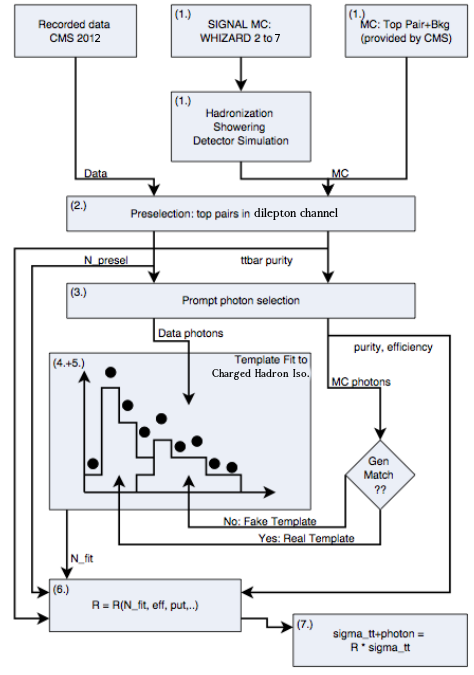
\includegraphics[width=0.75\textwidth]{Figures/AnalysisFlowChart2.png}
\end{center}
\caption{Flow chart showing each stage of the analysis. The box numbers represent the outlined
analysis steps.}
\label{fig-AnalysisFlowChart}
\end{figure}

\section{Pre-selection: Selection of $t\bar{t}$ Events} \label{sec-preselection}

The pre-selection steps define a sample of $t\bar{t}$ events before requiring the presence of a radiated photon. The selection follows the recommended selection from the TOP Reference Selections and Recommendations (Run 1) \cite{TopEventSelection} designed to select dilepton final states with two isolated oppositely charged leptons, at least 2 jets where at least one is a b-tagged jet, and missing transverse energy to account for the two neutrinos produced in W boson decay alongside the leptons. All objects in the selection are reconstructed using the PF algorithm as described in Section \ref{subsec-PFAlgorithm}.  

The steps for selecting di-muon and di-electron events are as follows:  

\begin{itemize}
	\item Skim
	\item Event cleaning and trigger
	\item dilepton selection
	\item Z-mass veto
	\item $\geq 1$ jet
	\item $\geq 2$ jets
	\item Missing transverse energy selection
	\item $\geq 1$ CSV b-jet 
\end{itemize}

For the mixed channel events are selected with two oppositely signed leptons, where one is an electron and the other a muon. Due to the final state containing different flavour leptons, the number of events stemming from the Drell-Yan process is significantly reduced, and therefore there is no need for a Z-mass veto such that is used for the same flavour lepton channels. For the same reason, there is no requirement for a cut on the missing transverse energy. The event selection for mixed final state event topologies are as shown below:

\begin{itemize}
	\item Skim
	\item Event cleaning and trigger
	\item dilepton selection
	\item $\geq 1$ jet
	\item $\geq 2$ jets
	\item $\geq 1$ CSV b-jet 
\end{itemize}  

Each step will be discussed in greater detail within the following sections. 

\section{Skim}

As mentioned above, we introduce a ``skim" in order to reduce the number of events, and thus size of ntuples, for offline analysis. Implementing a skim reduces computing time considerably. For the skim, we require the following set of nominal selection cuts:

\begin{itemize}
	\item The requirement of at least two leptons, excluding $\tau$ leptons.
	\item Electrons are defined as loose electrons and are required to have a transverse momentum of $p_T(e) > 20$ GeV and lie in the pseudorapidity range $|\eta(e)| < 2.5$.
	\item Muons are defined as loose electrons and are required to have a transverse momentum of $p_T(\mu) > 20$ GeV and lie in the pseudorapidity range $|\eta(\mu)| < 2.4$.
	\item Jets are required to have a transverse momentum of $p_T(jet) > 30$ GeV and lie within a pseudorapitiy range of $|\eta(jet)| < 2.6$.
\end{itemize}

\section{Trigger and Event Cleaning} \label{sec-TriggerAndEventCleaning}

\subsection{Trigger selection}

As the $t\bar{t}+\gamma$ analysis is studied as a dilepton final state, the requirement of at least two oppositely charged leptons (electrons or muons only) is essential. These datasets are identified by the trigger system (as described in Section \ref{sec-Trigger}) to contain two leptons. Triggers are generally divided into two categories: single object triggers fire on one or more objects of the same flavour passing certain pre-selection requirements, such as p$_T$ and $\eta$, and cross-triggers that select two objects of different flavour as predetermined by the user. For this analysis, both types of triggers are implemented in order to select the three final states in question. The list of trigger paths can be seen in Table \ref{tab-HLTriggers}. 

\begin{table} 
\begin{center}
\begin{tabular}{|c|p{11.5cm}|}
\hline
	\textbf{Final State} & \textbf{High Level Trigger Path} \\
\hline
	$\mu^+\mu^-$ & HLT\_Mu17\_Mu8\_v* \\
	$e^+e^-$ & HLT\_Ele17\_CaloIdT\_CaloIsoVL\_TrkIdVL\_TrkIsoVL
				\_Ele8\_CaloIdT\_CaloIsoVL\_TrkIdVL\_TrkIsoVL\_v* \\
	$e\mu$ & HLT\_Mu17\_Ele8\_CaloIdT\_CaloIsoVL\_TrkIdVL\_TrkIsoVL\_v*, HLT\_Mu8\_Ele17\_CaloIdT\_CaloIsoVL\_TrkIdVL\_TrkIsoVL\_v* \\
\hline	
\end{tabular}
\end{center}
\caption{Triggers for each dilepton channel.}
\label{tab-HLTriggers}
\end{table}

Each trigger path name explains the selection requirements on the objects that it triggers on. The first term in the trigger path, in this case HLT, refers to the Higher Level Trigger which is described in Section \ref{sec-Trigger}. The term Mu refers to a reconstructed muon and Ele refers to a reconstructed electron, where the succeeding number represents an associated energy threshold for the particle. For example, the the di-muon channel uses a single flavour object trigger to select two muons and is used with the requirements that one of the muons has a p$_T$ greater than 8 $\GeV$ and the second greater than 17 $\GeV$. The version of the trigger is denoted in the trigger path as v*, as the trigger path changes with the trigger table used. It should be noted that a different trigger version does not in fact require a change in trigger path. At this level the number of energy deposits within the calorimetry is still too large for the trigger rate to be usable, and thus extra selection requirements on top of those required by the trigger system must be imposed.

One way to reduce the trigger rate is to impose a selection requirement on the transverse momentum threshold of the particles in question greater than that required by the trigger; however, this holds drawbacks for analyses that then wish to implement more stringent selection requirements within offline analysis. Another method, and one that is used primarily in electron trigger studies, is to reduce trigger rates to a more feasible level by introducing isolation and identification requirements; these are indicated by the `Iso' and `Id' terms that can be seen in the di-electron and $e\mu$ trigger path names. The objects must then also pass simple isolation and identification criteria, thus reducing the trigger rate. The information for each is obtained from both the calorimeter (e.g CaloIso) and tracker (e.g TrkId) by placing requirements on such parameters as the shape of the energy cluster in the ECAL, the total number of energy depositions in the ECAL, and the angular separation between the ECAL and tracker-energy deposits. Three categories of selection are implemented for each kinematic selection requirement, and are listed as Tight (T), Loose (L), and Very Loose (VL) as can be seen in the trigger paths. These signify the harshness of the cuts when applied. This can be visualised, for example, in the di-electron channel where the HLT calls for two electrons, where one must pass an transverse momentum threshold of 8 $\GeV$ with a tight requirement on calorimeter identification, and very loose requirements on calorimeter isolation and tracker identification and isolation. The other electron must pass an transverse momentum threshold of 17 $\GeV$ with the same calorimeter and tracker isolation and identification requirements.

HLTs paths are used for the $t\bar{t}+\gamma$ analysis such that if the event does not pass the requirement of the trigger, then it is not included in the result. Single object triggers are used for both the di-muon and di-electron channels, and two cross-triggers were used for the $e\mu$ channel as the final state selection requires two oppositely charged leptons (electrons or muons) where one is an electron and the other a muon. The triggers were processed specifically for the $\sqrt{s}=8 \TeV$ data-taking period that corresponds to an integrated luminosity of 19.6 $\fbinv$.

\subsection{Filtering}

Known anomalies derived from detector and accelerator effects have to be accounted for in the processing of data. To counter these effects, several `cleaning' filters are incorporated after trigger selection, but before any further selection cuts are applied. The first of these replicates \textbf{beam scraping} by including a \textbf{tight CSC Beam Halo Filter}. We find that, even with the accuracy and precision that the LHC provides on accelerating bunches of protons, protons have a tendency to diverge radially from the bunch and form what is known as the beam halo that circulates the accelerator with each bunch. In early analyses it was found that the beam halo particles can be picked up in the detectors and be reconstructed as part of an event. Due to sensitivity to beam halo particles in the muon detectors, a filter is introduced based on muon tracking kinematics that allows these events to be vetoed. Beam halo particles can also be removed from the beam within the LHC by introducing collimating blocks around the beam line at various points around the accelerator. This, however, presents another problem in the form of showering as the particles interact with the collimator blocks, and are then detected by the experiments. This is known as beam scraping. These events are accounted for and removed from analyses by introducing the requirement that at least 25\% of reconstructed tracks within the inner detector pass the high purity threshold (see Section \ref{subsec-ChargedParticleTracking}). 

Similarly, a \textbf{HCAL noise filter} is employed in order to remove events with anomalous noise within the HCAL. CMS expects a certain degree of noise, stemming from the electronics of the detector, to be present when recording data, however the majority of anomalous noise in the HCAL is found to originate in the Hybrid Photo-Triodes (HPT) and their corresponding read-out boxes. At the current energy scale this is not a problem as the noise appears as large, isolated energy deposits. Anomalous events have easily-identifiable signatures such as the isolation of the noise within HCAL, and the multiplicity in the individual read-out boxes. So, if a signal demonstrates very little change in pulse shape over time, and the read-out boxes display a high multiplicity, then an event is rejected. The next filter comes in the form of the \textbf{HCAL laser filter}. The need for the laser filter first manifested during the 2011 data taking period when a much greater number of hits per event was observed than was expected: approximately 5000 per event. The HCAL laser filter was then designed and introduced for the 2012 data taking period.  

%%%%%%%%%%%%%%%%%%More

\section{Dilepton Selection and Vetoes}

For the $t\bar{t}+\gamma$ analysis, leptons form a key part of the signature in the final state. The leptons are taken from the list of PF-reconstructed objects and then required to pass additional selection requirements to refine the events further after the trigger selection described in Section \ref{sec-TriggerAndEventCleaning} has been applied. Along with the signal leptons, a set of `looser' PF objects are selected as veto objects, such that the signal leptons are a subset of these objects. If an event has multiple loose selection leptons then the event is removed from the list of possible signal candidates.

The number of selected leptons differs for each decay mode, and thus three separate sets of selection criteria must be created for the di-muon, di-electron, and mixed channels, respectively. Selection requirements on the leptons vary depending on the channel, but are taken from the recommended values produced by the central `Top Event Selection' group \cite{TopEventSelection}. 

\subsection{Electrons}

PF electron candidates are selected for the di-electron and $e\mu$ channel if they have been identified using the GSF method, as described in Section \ref{subsec-ElectronIdentification}, and pass the HLT for each channel, respectively. The purity of top pair events is then improved by imposing a further set of selection requirements taken from the recommended top reference selection \cite{TOPEGM1}. The selection requirements for a ``tight" electron are as follows:

\begin{itemize}
	\item Electrons must satisfy a p$_T$ threshold of > 20 \GeV.
	\item Electrons must lie within the pseudorapidity region $|\eta| < 2.5$, excluding the EB-EE transition region $1.4442 < |\eta| < 1.5660$;
	\item The transverse IP of the electron (GSF) track with respect to the first offline primary vertex must be less than 0.04 cm; 
	\item The combined relative Particle Flow (PF) $\rho$-corrected isolation in a cone of radius 0.3 must be less than 0.15;
	\item The trigger version of the electron multivariate discriminator Trigger MVAID must be greater than 0.5;
	\item Conversion rejection: there should be no extra tracks pointing in the same direction;
	\item The ratio of energy deposited in the HCAL over the energy deposited in the ECAL to be less than 0.05.
\end{itemize} 

For electrons, an additional identification process is included, which uses a multivariate analysis to combine the information from several variables to produce a discriminator value between -1 and 1, such that the greater the number the more likely the object is to be an electron (as described in Section \ref{subsec-ElectronIdentification}). Depending on whether the HLT requires an electron or not, a different version of the discriminant is used. 

One of the main criteria for lepton selection is the requirement of isolation. Generally, the isolation is defined to be the sum of the p$_T$ of the reconstructed objects within a cone by which we define the radius, and then dividing by the p$_T$ of the object. If it is found that this produced a small number, then it is said that the object is isolated. It is necessary to include the effect of event PU into the calculation of isolation, and thus introduce a correction factor. It is then possible to remove charged hadron tracks from the isolation sum if they do not originate from the event's primary vertex. For the case of neutral hadrons and photons that originate from PU, an effective area is defined for the electron and then an average energy is subtracted over this area. For electrons, the isolation is defined as follows:

\begin{equation} \label{eq-RelativeIsolation}
I_{\rho} = \frac{I_{ChargedHadron}+max\left(I_{NeutralHadron} + I_{\gamma} - \rho \cdot Eff.Area_{electron}, 0 \right)}{p_T}
\end{equation}

such that $I_{ChargedHadron}$, $I_{NeutralHadron}$, and $I_{\gamma}$ are the are the isolation cones with a fixed radius of $\Delta R = 0.3$ containing the energy deposits for each category of particle: charged hadron, neutral hadron, and photon. The $\rho$ and $Eff.Area_{electron}$ parameters are the energy density of the event and the effective area for the electron which is calculated by taking the supercluster pseudorapidity $\eta_{SC}$ and electron p$_T$. 

When a photon produced in collisions interacts with the detector material of the inner tracker it can pair-produce two electrons, thus mimicking the signature of an electron: this is known as a conversion. This has been found to represent a large source of fake electrons. The CMS EGamma working group have developed two methods in order to mitigate this effect: measuring missing hits within the tracker system and measuring associated secondary tracks. The first technique measures the number of hits in the layers of the tracker and looks for any missing hits in the electron's associated track. If there are any missing hits, then the electron is considered to be a conversion, and is discarded. The second method requires a secondary electron/positron track such that it reconstructs the pair under a certain criteria: if that second track is not found to be within 0.02 cm in the $r - \phi$ plane and the $\cot\theta$ between the two tracks differs by less than 0.02 then the electron is considered a conversion. 

A set of loose electron candidates is defined by applying the recommended cuts as for signal electrons but with less stringent requirements, such that the signal electrons are a subset of the loose electrons. \textbf{Loose electrons} are defined to have the following cuts:

\begin{itemize}
	\item Transverse momentum $p_T$ greater than 10 GeV;
	\item Absolute value of pseudorapidity less than 2.5;
	\item Combined relative Particle Flow (PF) $\rho$ corrected isolation in cone 0.3 less than 0.15;
	\item Trigger version of electron multivariate discriminator: Non-Trigger MVAID greater than 0.
\end{itemize}

\subsection{Muons}

For the \textbf{signal muons}, once they have passed the PF selection described in Section \ref{subsec-MuonReconstruction}, additional requirements taken from the recommended Muon Physics Object Group (POG) \cite{TOPMUO1} are imposed as follows:

\begin{itemize}
	\item Transverse momentum p$_T$ greater than 20 \GeV;
	\item Muons must lies within the pseudorapidity region $|\eta| < 2.4$, excluding the EB-EE transition region $1.4442 < |\eta| < 1.5660$;
	\item The combined relative Particle Flow (PF) $\rho$-corrected isolation in cone 0.4 must be less than 0.2;
	% \item at least 5 hits in the tracker (with at least one coming from the pixel detector)
	% \item At least one hit in the muon detector
	\item Identified as a particle flow muon;
	\item Identified as both a tracker and global muon.
\end{itemize}

The relative isolation for the signal muon candidates is pileup correction, which is much less complicated to compute than electron relative isolation. The technique for computing muon relative isolation by way of pileup correction is known as $\Delta \beta$ correction and removes the neutral hadron and photon isolation from the isolation sum within a fixed cone of radius $\Delta R = 0.4$. The relative isolation for muons can be computed as follows:

\begin{equation}
I_{\Delta \beta} = \frac{I_{ChargedHadron} + max\left(I_{NeutralHadron} + I_{\gamma} - 0.5 \cdot I_{Pileup}, 0 \right)}{p_T}
\end{equation}

where the $I_{Pileup}$ parameter is the neutral hadron energy within the cone, and the factor of 0.5 is a rough estimate of the ratio of neutral hadron to charged hadron in pileup events. Muons are categorised as being isolated if it satisfies $I_{\Delta \beta} < 0.2$ within an isolation cone of $\Delta R = 0.4$. 

The production of muons from in-flight decays is found to be much more prominent in data than in simulation. This results in a number of fake muons being recorded. In order to account for the number of fakes, the implementation of further selection requirements is needed, such that at least one hit is required in each of the pixel detector and muon detector, and that at least 6 hits are recorded in the inner tracking system, with two corresponding hits in the outer muon system (the drift tubes).  

\textbf{Loose Muons} are selected from PF muons failing the muon selection that have, and are selected to have, less severe requirements as listed below:

\begin{itemize}
	\item Transverse momentum $p_T$ greater than 10 GeV;
	\item Absolute value of pseudorapidity less than 2.5;
	\item Combined relative Particle Flow (PF) $\rho$ corrected isolation in cone 0.4 less than 0.2;
	% \item At least 5 hits in the tracker (with at least one coming from the pixel detector)
	% \item At least one hit in the muon detector
	\item Identified as a particle flow muon;
	\item Identified as both a tracker and global muon.
\end{itemize}

The lead and second lepton transverse momentum distributions, along with the invariant mass of the two selected leptons, are shown in Figure \ref{fig-leptonPlots}. All other dilepton kinematic and mass distributions can be seen in Figure \ref{subsec-leptonPlots}, and we see a good agreement between the data and simulation.

\begin{figure}
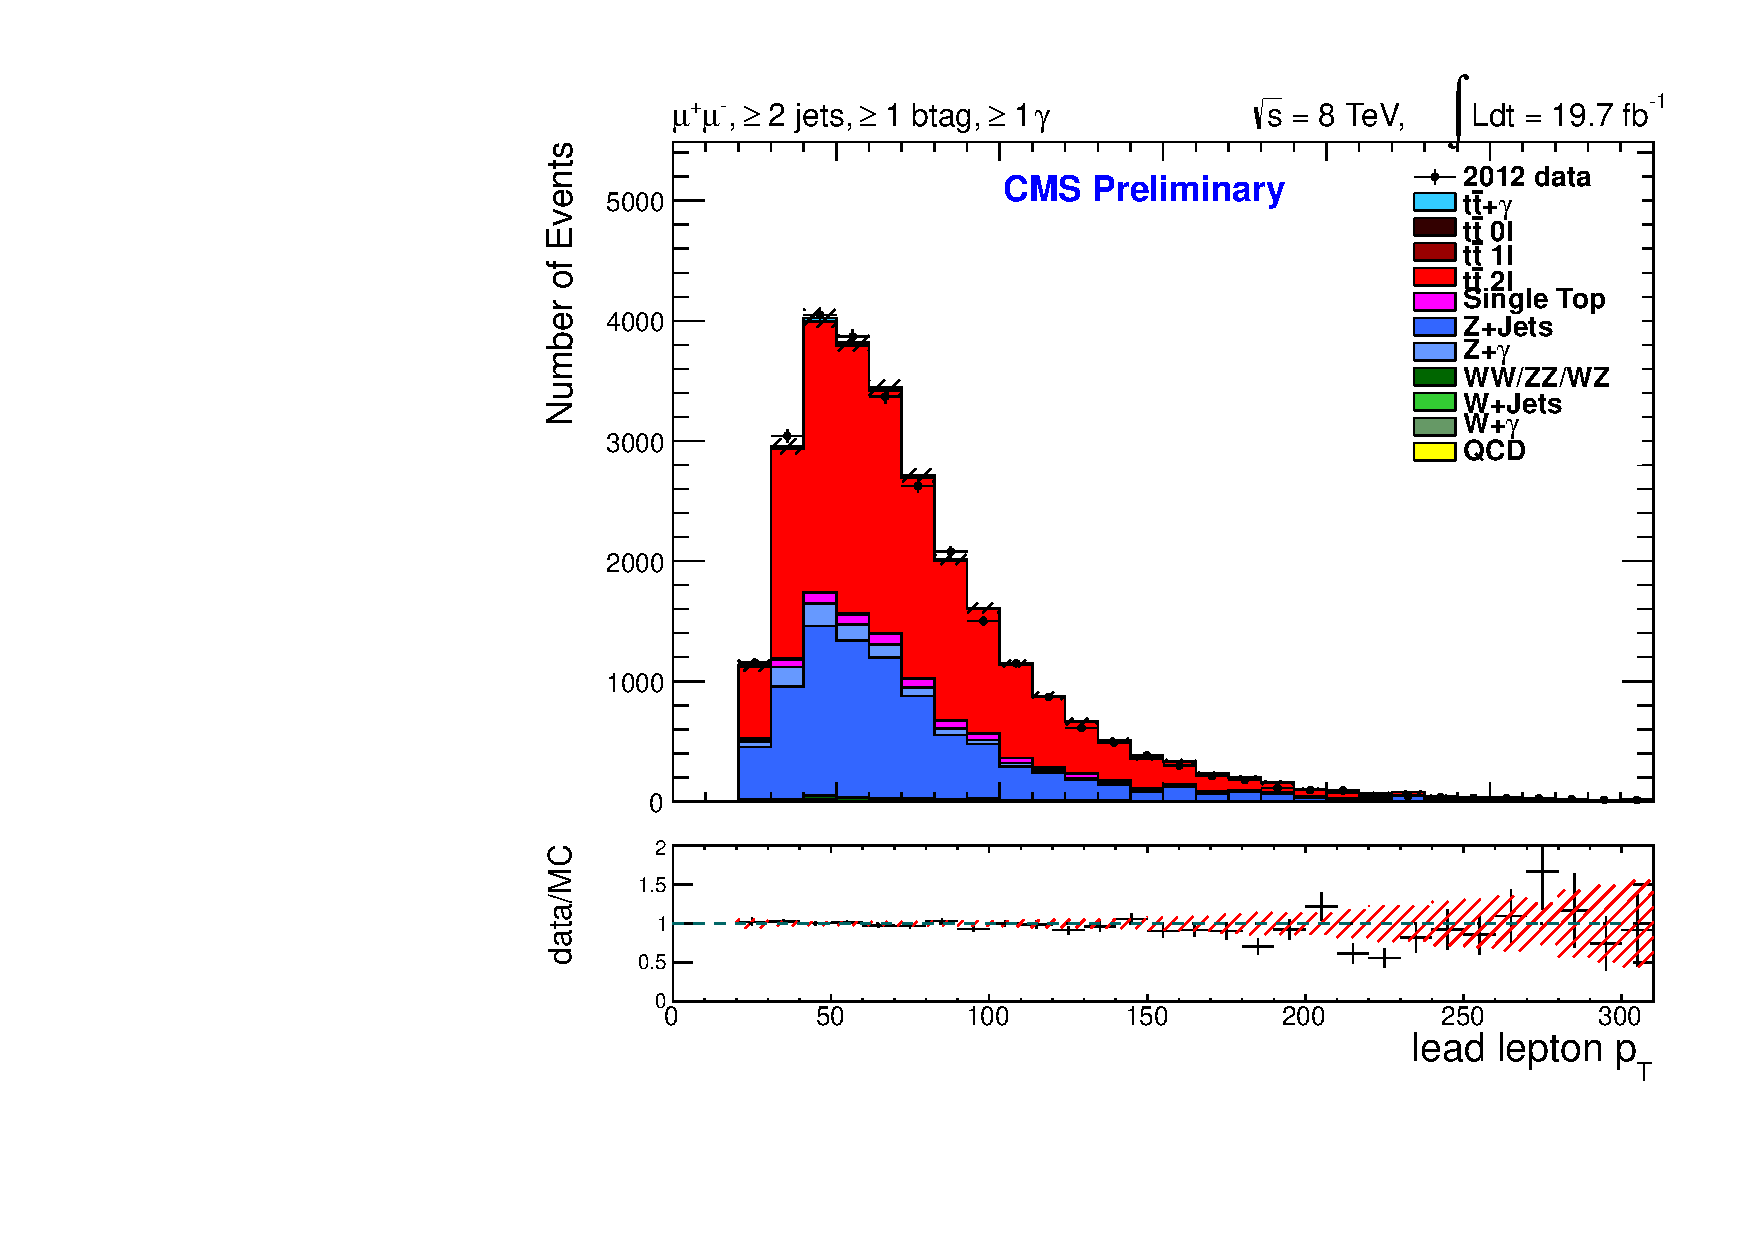
\includegraphics[width=0.5\textwidth]{Plots/ControlPlots/TTbarDiLeptonAnalysis/MuMu/DiLepton/LeadLepton_Pt_splitTTbar_ratio.pdf}
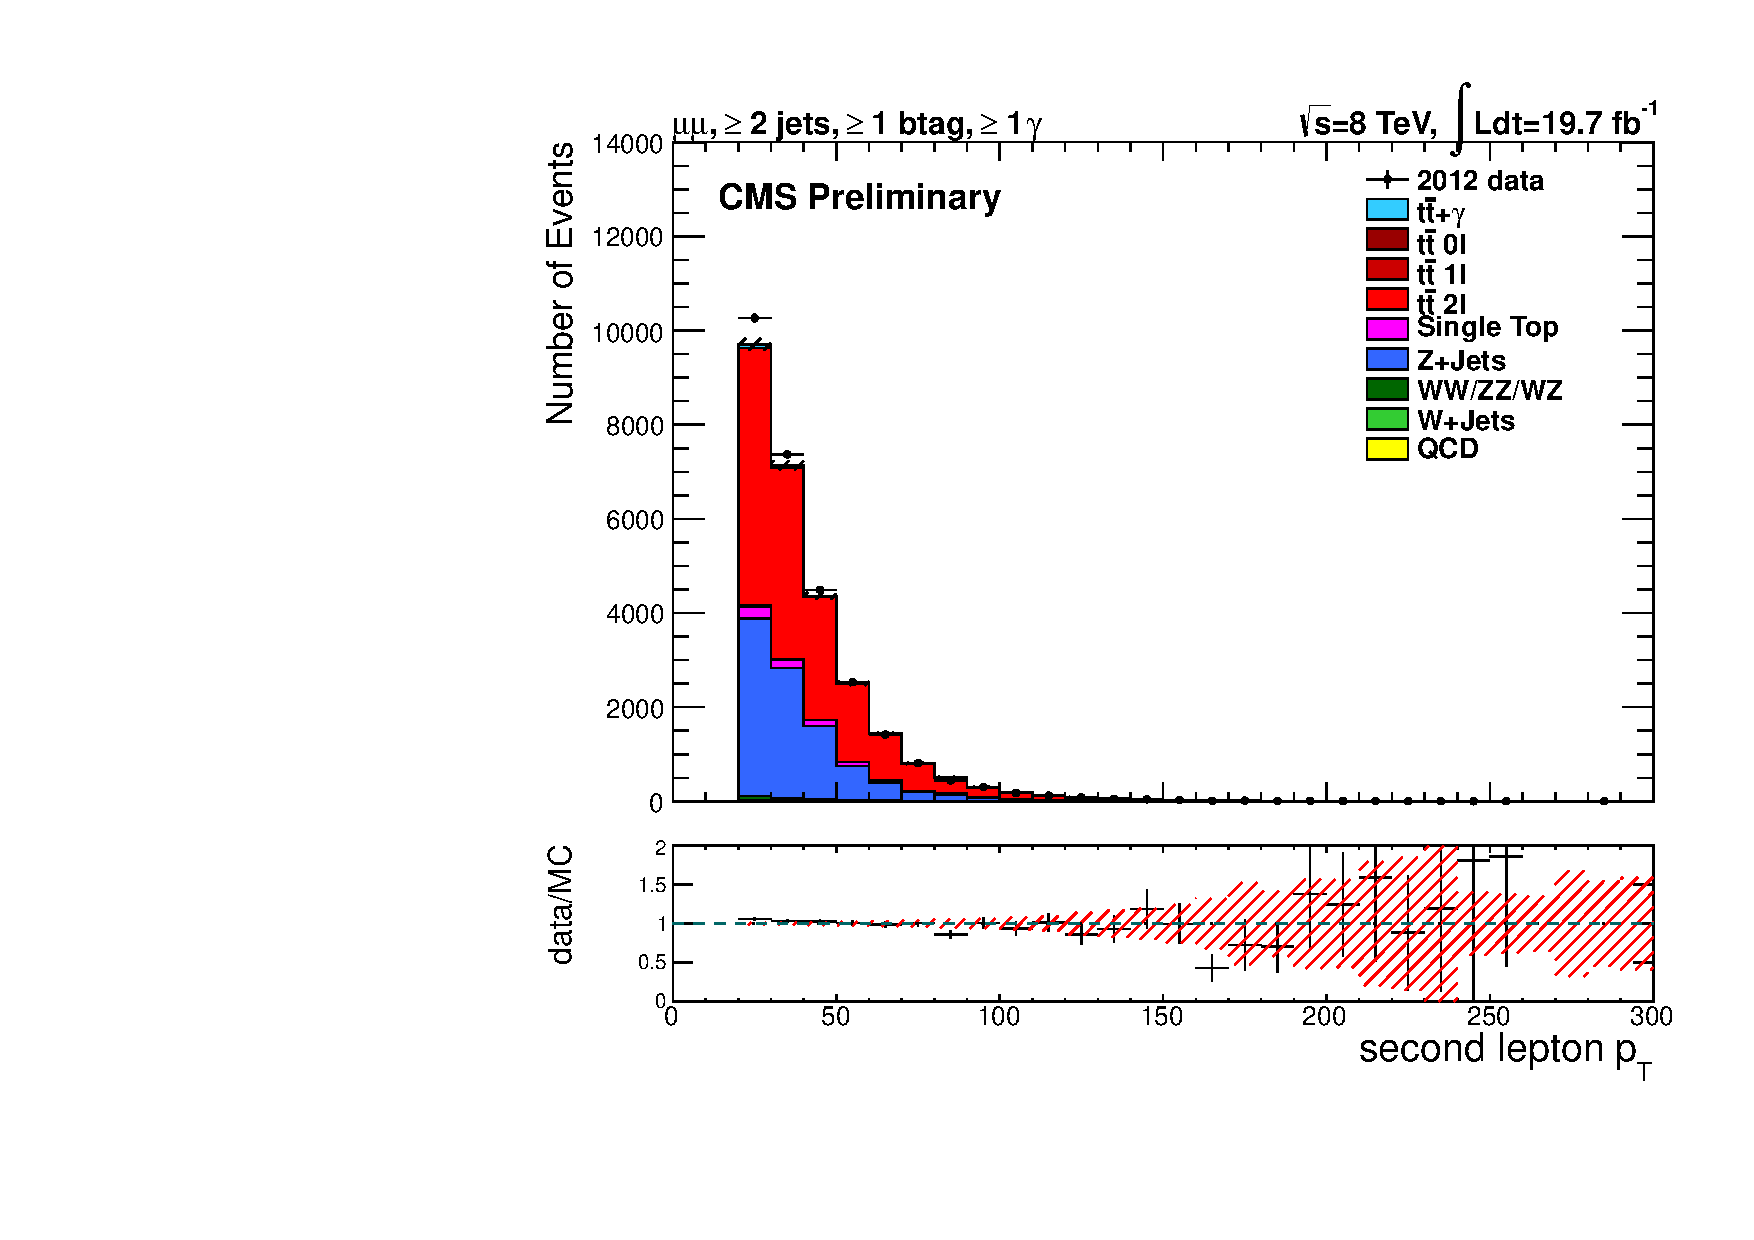
\includegraphics[width=0.5\textwidth]{Plots/ControlPlots/TTbarDiLeptonAnalysis/MuMu/DiLepton/SecondLepton_Pt_splitTTbar_ratio.pdf}\\
\begin{center}
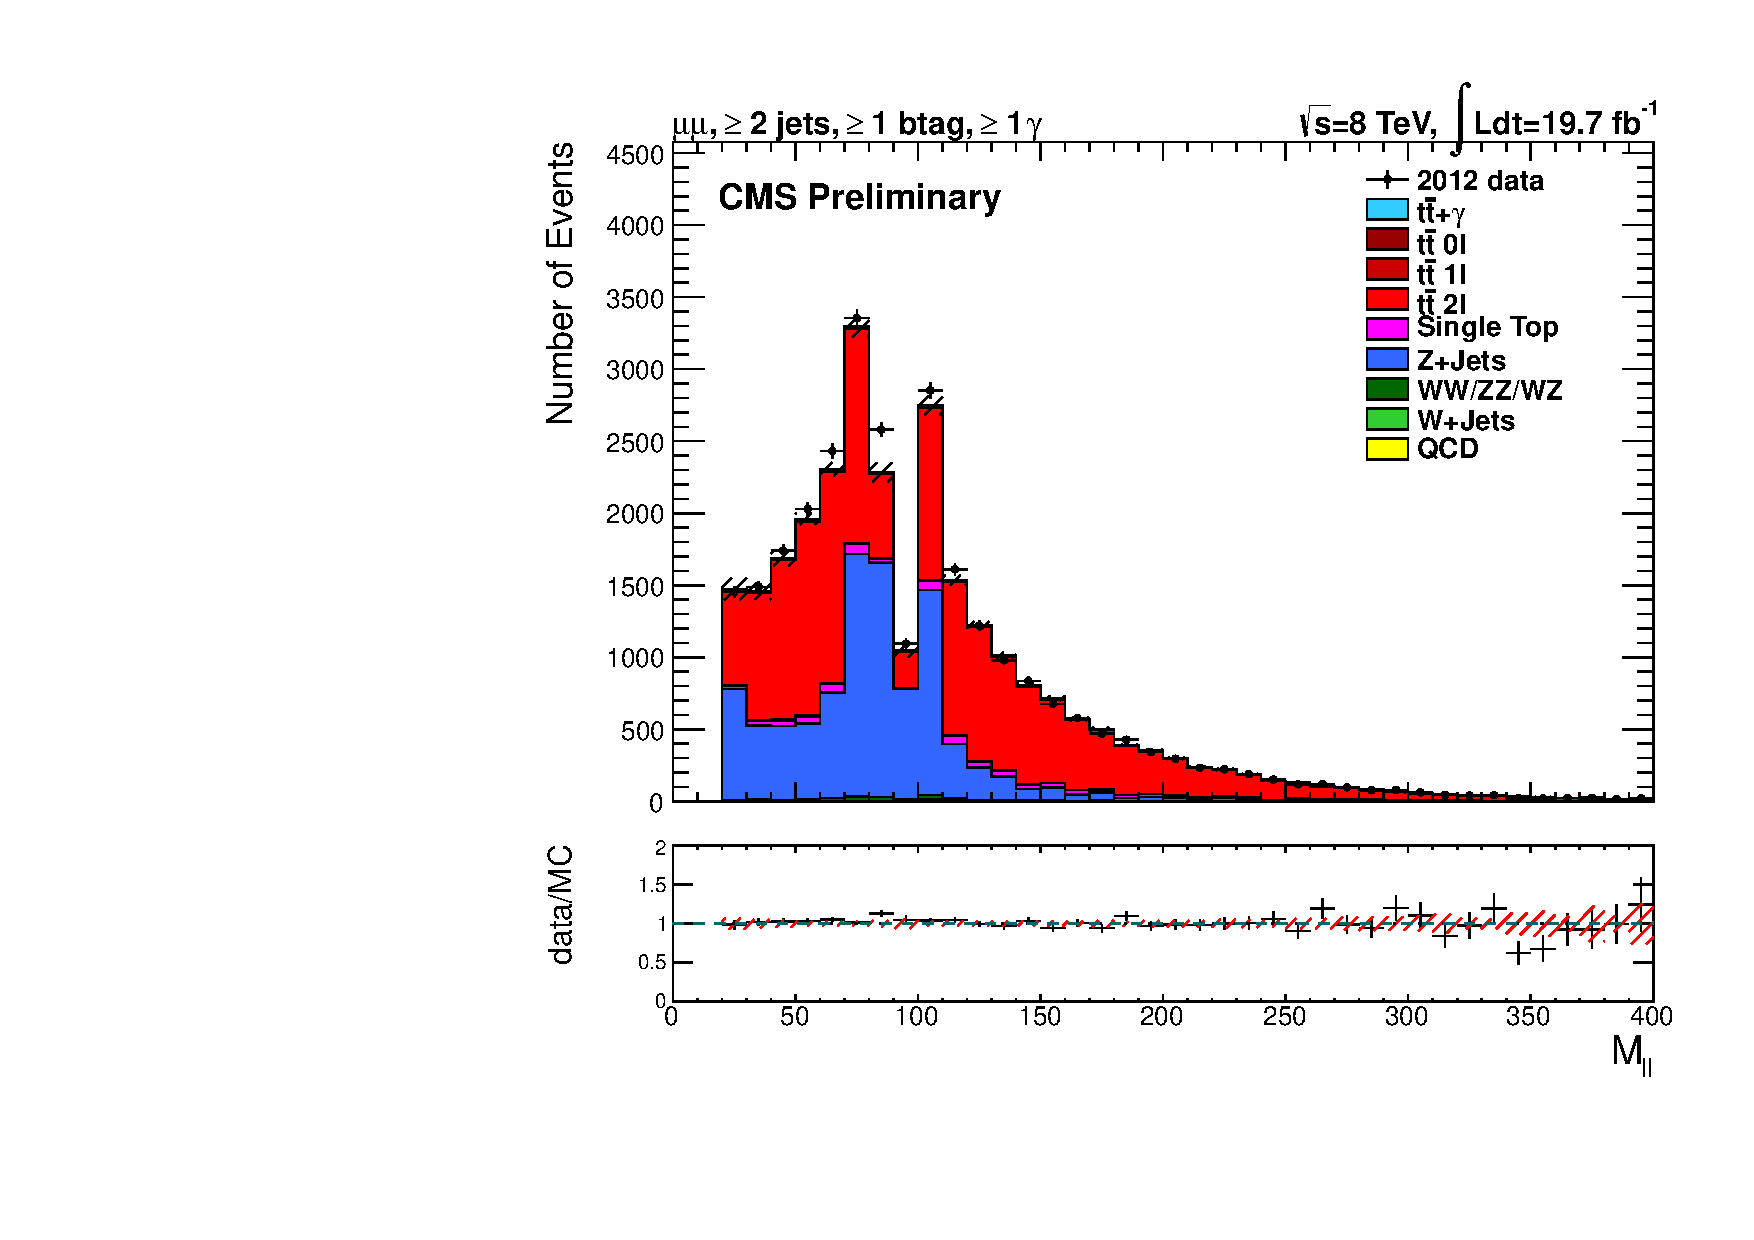
\includegraphics[width=0.5\textwidth]{Plots/ControlPlots/TTbarDiLeptonAnalysis/MuMu/DiLepton/diLepton_Mass_splitTTbar_ratio.pdf}
\end{center}
\caption{Lead lepton p$_T$ (top left), second lepton p$_T$ (top right), and dilepton mass (bottom) for the $\mu^{+}\mu^{-}$ channel only after $t\bar{t}$ selection.}
\label{fig-leptonPlots}
\end{figure}

\section{Jet Selection and b-tag Requirements} \label{sec-JetSelection}

Jets are reconstructed with the AK5 PF algorithm, which is the anti-$k_T$ algorithm with jet size parameter (R) of 5 in the jet reconstruction model. Before applying any selection the following corrections are made to account for imperfect jet energy measurement: Jet Energy Scale correction and Jet Energy Resolution smearing, as described in Section \ref{subsec-JetReconstruction}. After jets are identified and reconstructed, the following set of selection requirements are applied:

\begin{itemize}
	\item Transverse momentum greater than 30 GeV;
	\item Absolute value of pseudorapidity less than 2.4;
	\item Number of constituents greater than 1;
	\item Charge multiplicity greater than 0;
	\item Neutral hadron fraction of energy less than 0.99;
	\item Neutral electromagnetic energy fraction less than 0.99;
	\item Charged EM energy fraction less than 0.99;
	\item Charged hadron energy fraction greater than 0.
\end{itemize}

These selection requirements help to avoid picking up detector noise and ECAL spikes as jets. A selection criterion is also imposed such that if a lepton lies within a cone of $\Delta R = 0.3$ then the lepton is included within the jet calculation. CMS improves the quality of reconstructed jets by the requirement that the energy deposits from a jet are recorded in both the ECAL and HCAL, where jets that manifest from anomalous deposits of energy in just one of the sub-detector are able to be removed from the sample \cite{CMS-PAS-JME-10-003}. The jet transverse momentum, pseudorapidity, and number of jets in the di-muon channel can be seen in Figure \ref{fig-jetPlots}. All other variables for each decay channel can be seen in Section \ref{subsec-jetPlots}

 \textbf{B-tagged jets} are identified with the Combined Secondary Vertex b-tagging algorithm using the loose working point (CSVL). Event re-weighting is applied to correct for the difference in b-tagging efficiency between data and simulation as explained in Section \ref{sec-SimulatedEventsCorrection}. The loose working point refers to a b-tagging misidentification probability of 24.4\%.

 In each decay channel is the requirement of at least 2 good jets, where a good jet passes all the aforementioned selection requirements, where at least one of the jets is a b-tagged jet. By applying these requirements the contribution from the most prominent backgrounds, $t\bar{t}$ and events with additional loose jets, are removed. 

\begin{figure}
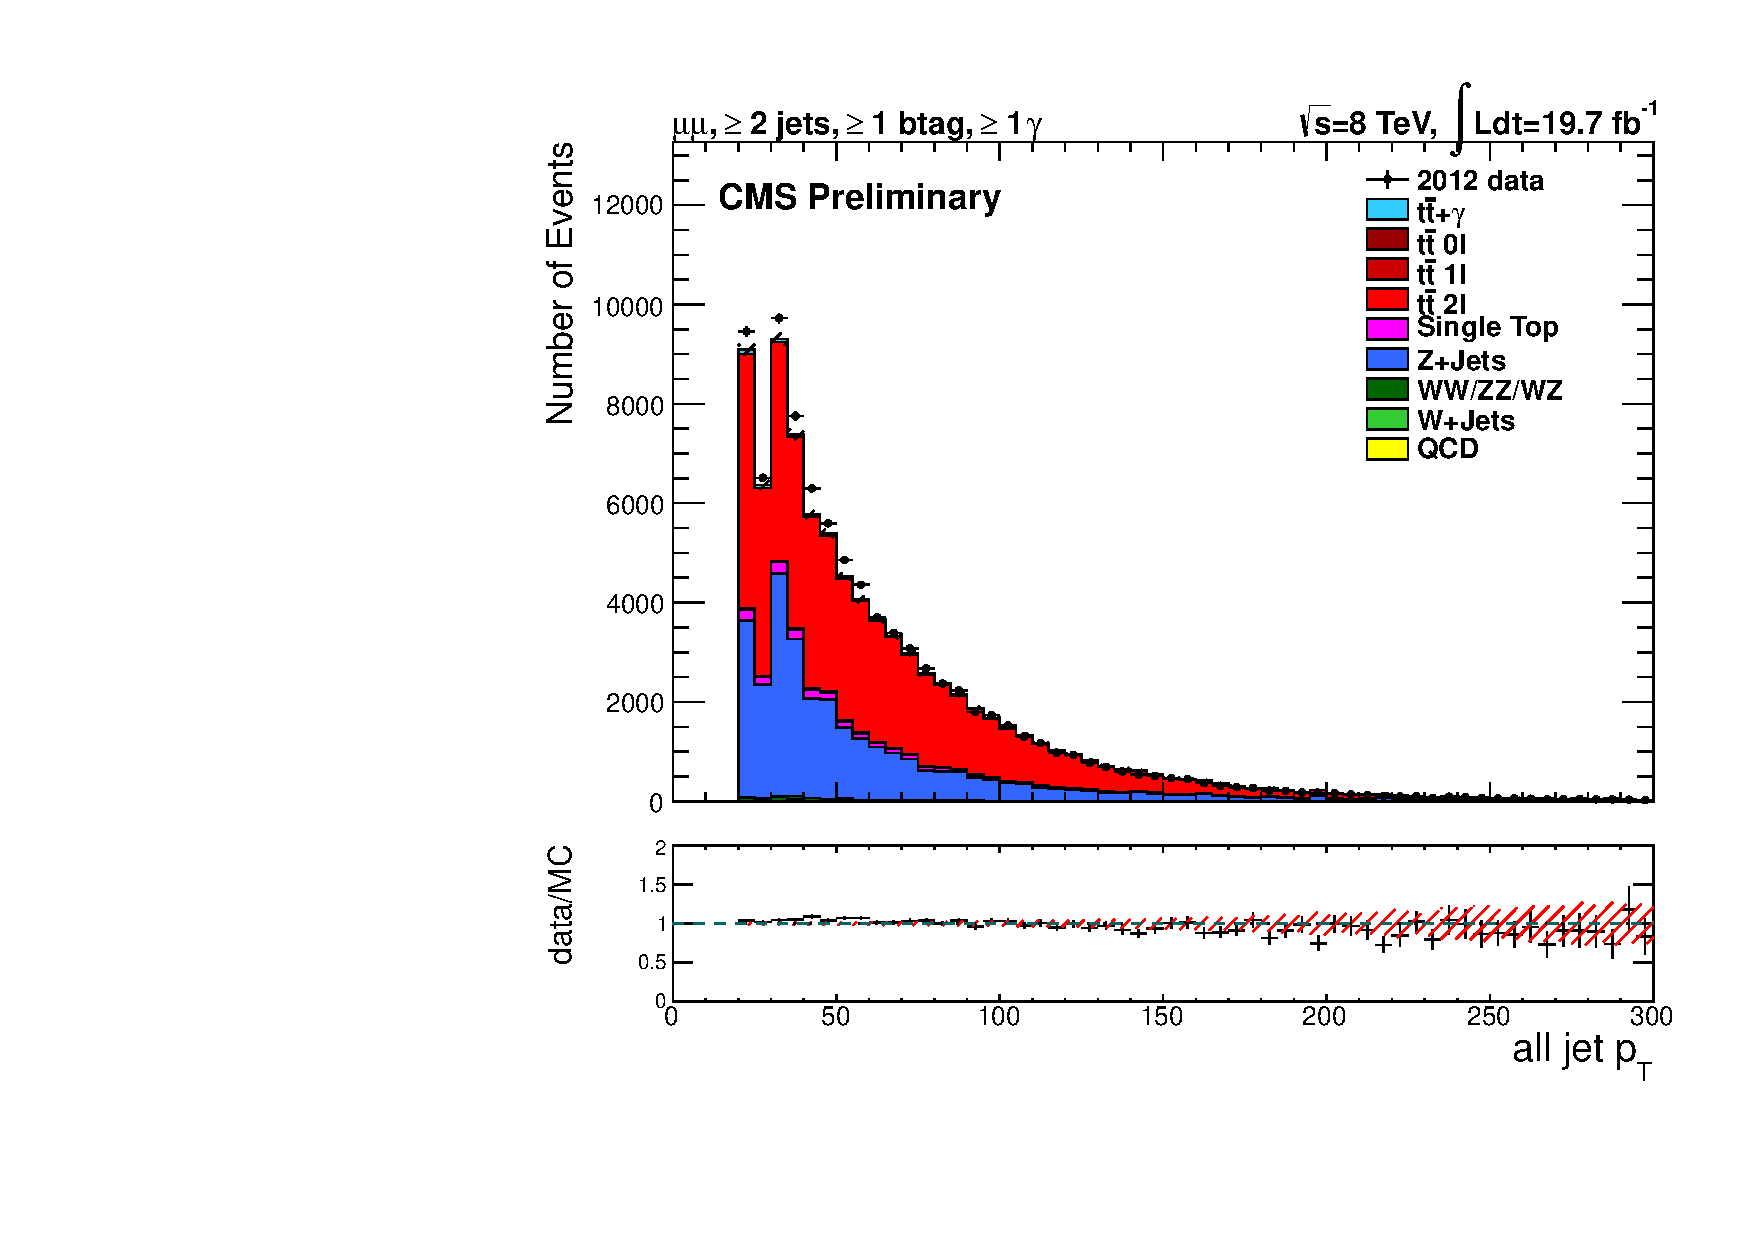
\includegraphics[width=0.5\textwidth]{Plots/ControlPlots/TTbarDiLeptonAnalysis/MuMu/Jets/all_jet_pT_splitTTbar_ratio.pdf}
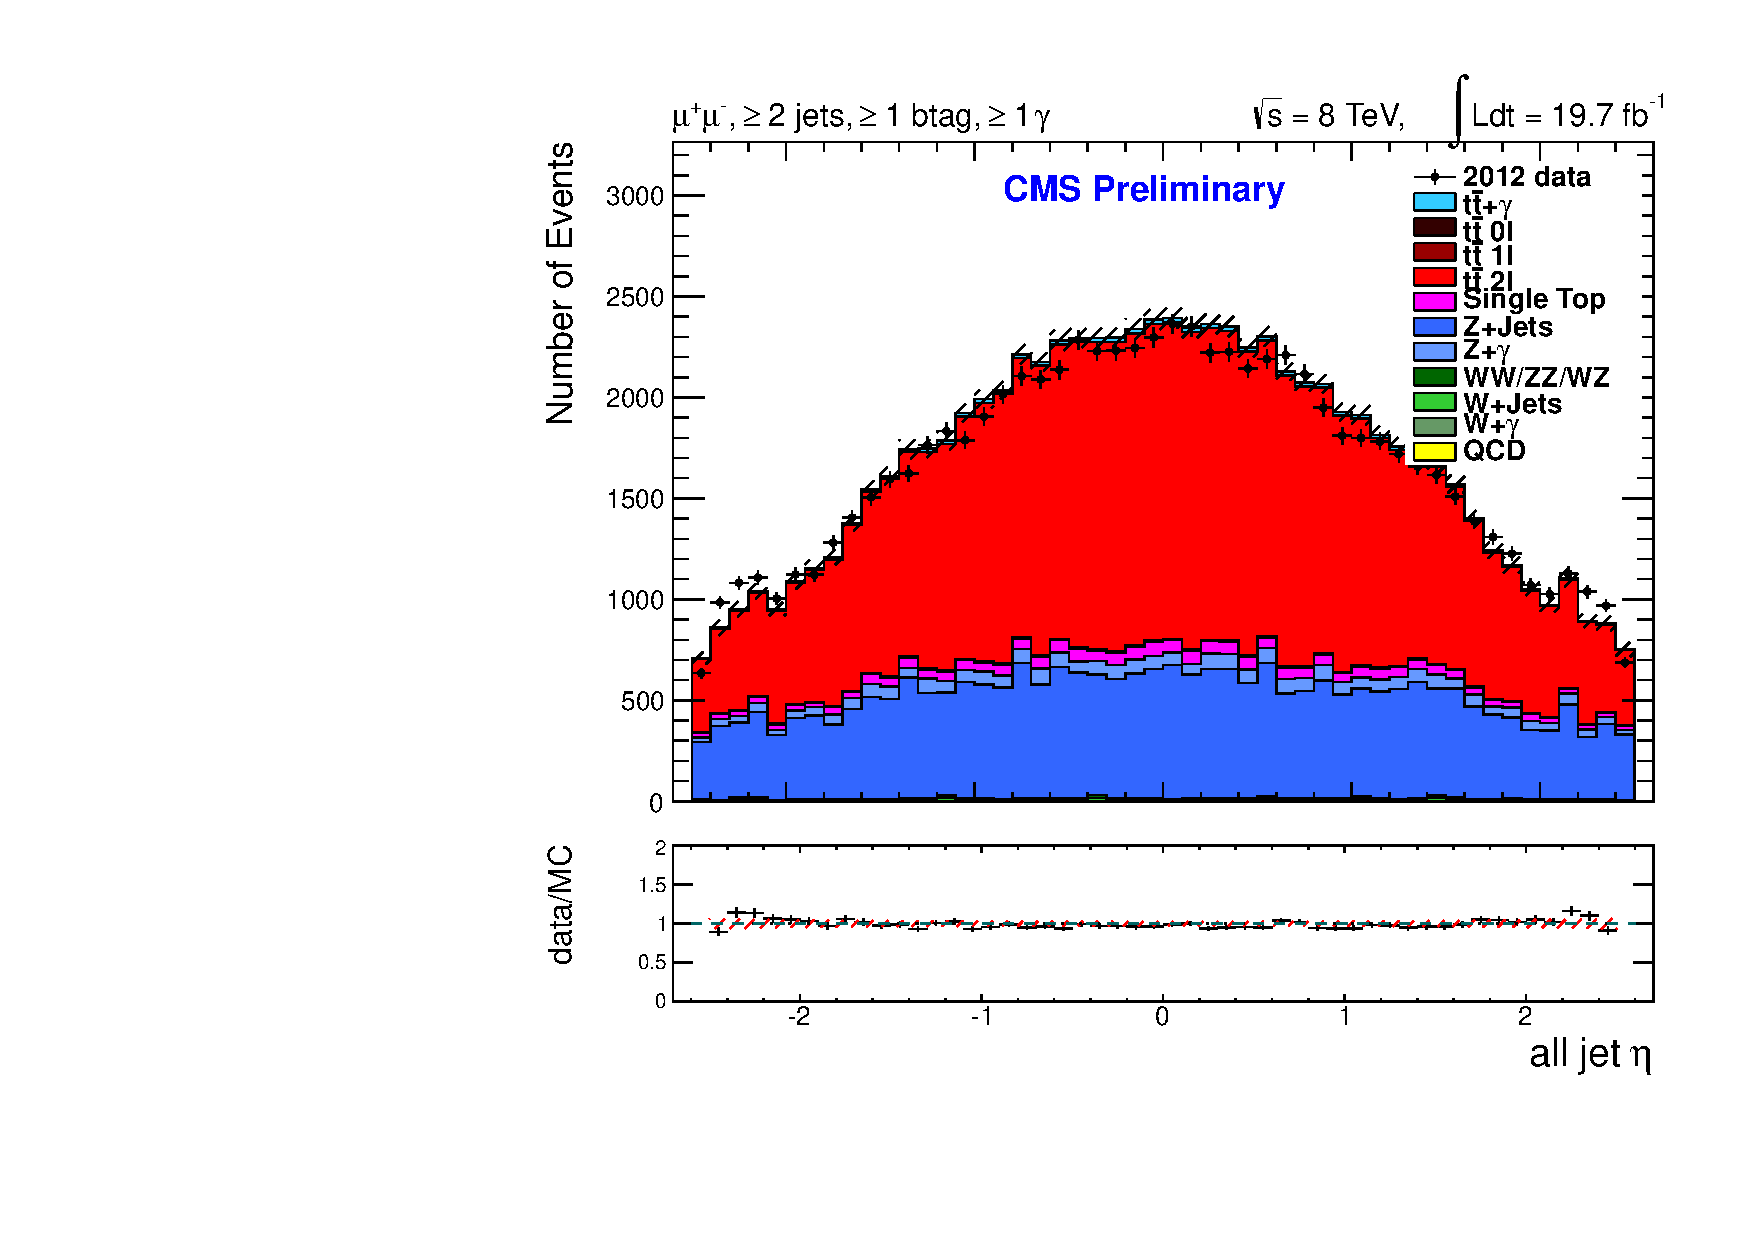
\includegraphics[width=0.5\textwidth]{Plots/ControlPlots/TTbarDiLeptonAnalysis/MuMu/Jets/all_jet_eta_splitTTbar_ratio.pdf}\\
\begin{center}
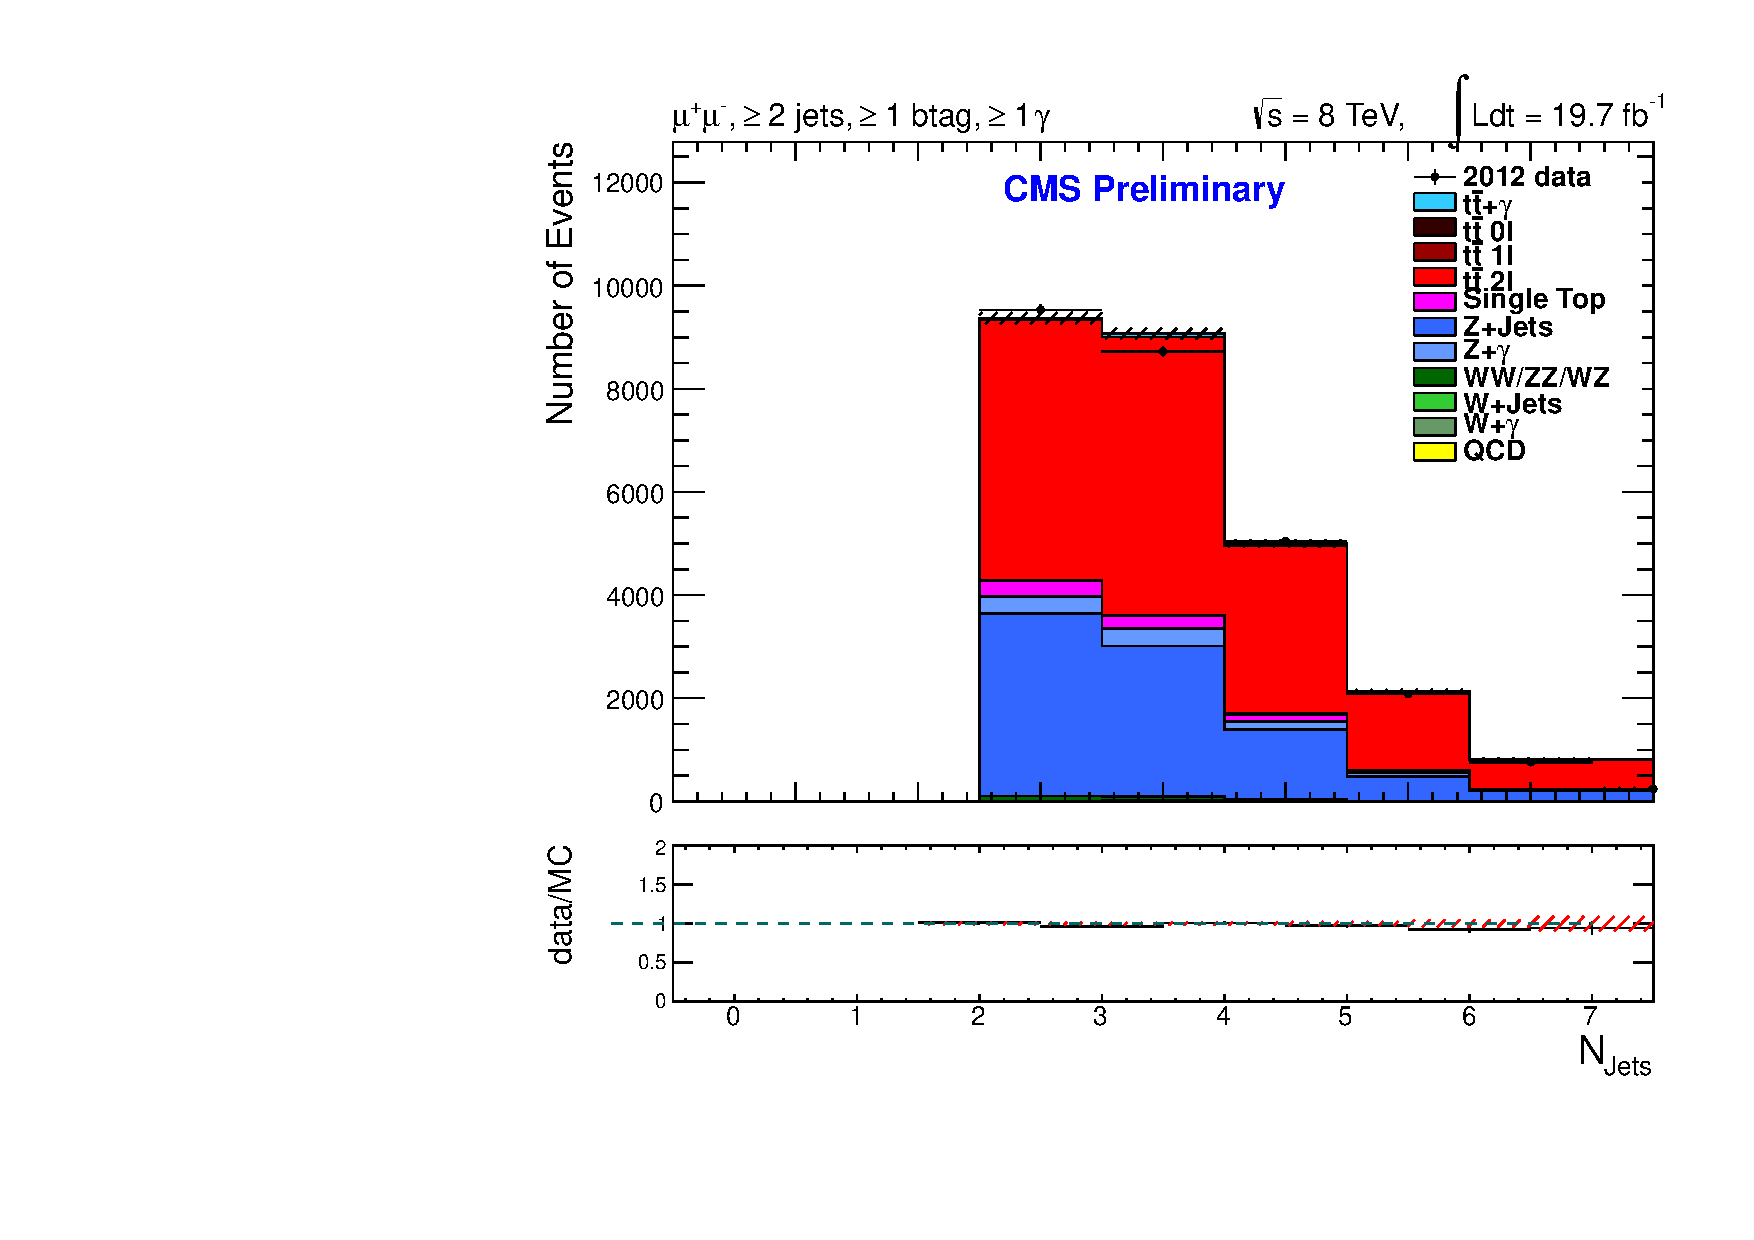
\includegraphics[width=0.5\textwidth]{Plots/ControlPlots/TTbarDiLeptonAnalysis/MuMu/Jets/N_Jets_splitTTbar_ratio.pdf}
\end{center}
\caption{Comparison of the sum of the transverse momentum and $\eta$ in all reconstructed jets (top), and number of jets (bottom) per event for the $\mu^{+}\mu^{-}$ channel only after $t\bar{t}$ selection.}
\label{fig-jetPlots}
\end{figure}
 
\section{Missing Transverse Energy} \label{sec-METSelection}

The missing transverse energy (MET) selection requirement is implemented only within the di-muon and di-electron channels as the mixed channel is better defined such that different flavour quarks in the final state reduce the contribution from Drell-Yann process considerably, and therefore less likely to be misreconstructed in the detector. Due to the small cross-section for the $t\bar{t}+\gamma$ process, and the much smaller branching ratio of the dilepton channel relative to the semileptonic channel, the requirement of $>20$ GeV, compared to the nominal 40 GeV, is imposed in order to increase statistics. Figure \ref{fig-METphiSig} shows the MET, the azimuthal angle $\phi$ of the MET, and the MET significance, where the MET significance assesses on an event-by-event basis the likelihood that an observed MET is consistent with a fluctuation from zero due to detector-related limitations, such as finite measurement resolution. The distributions for the other variables can be seen in Figure \ref{subsec-METPlots}.

\begin{figure}
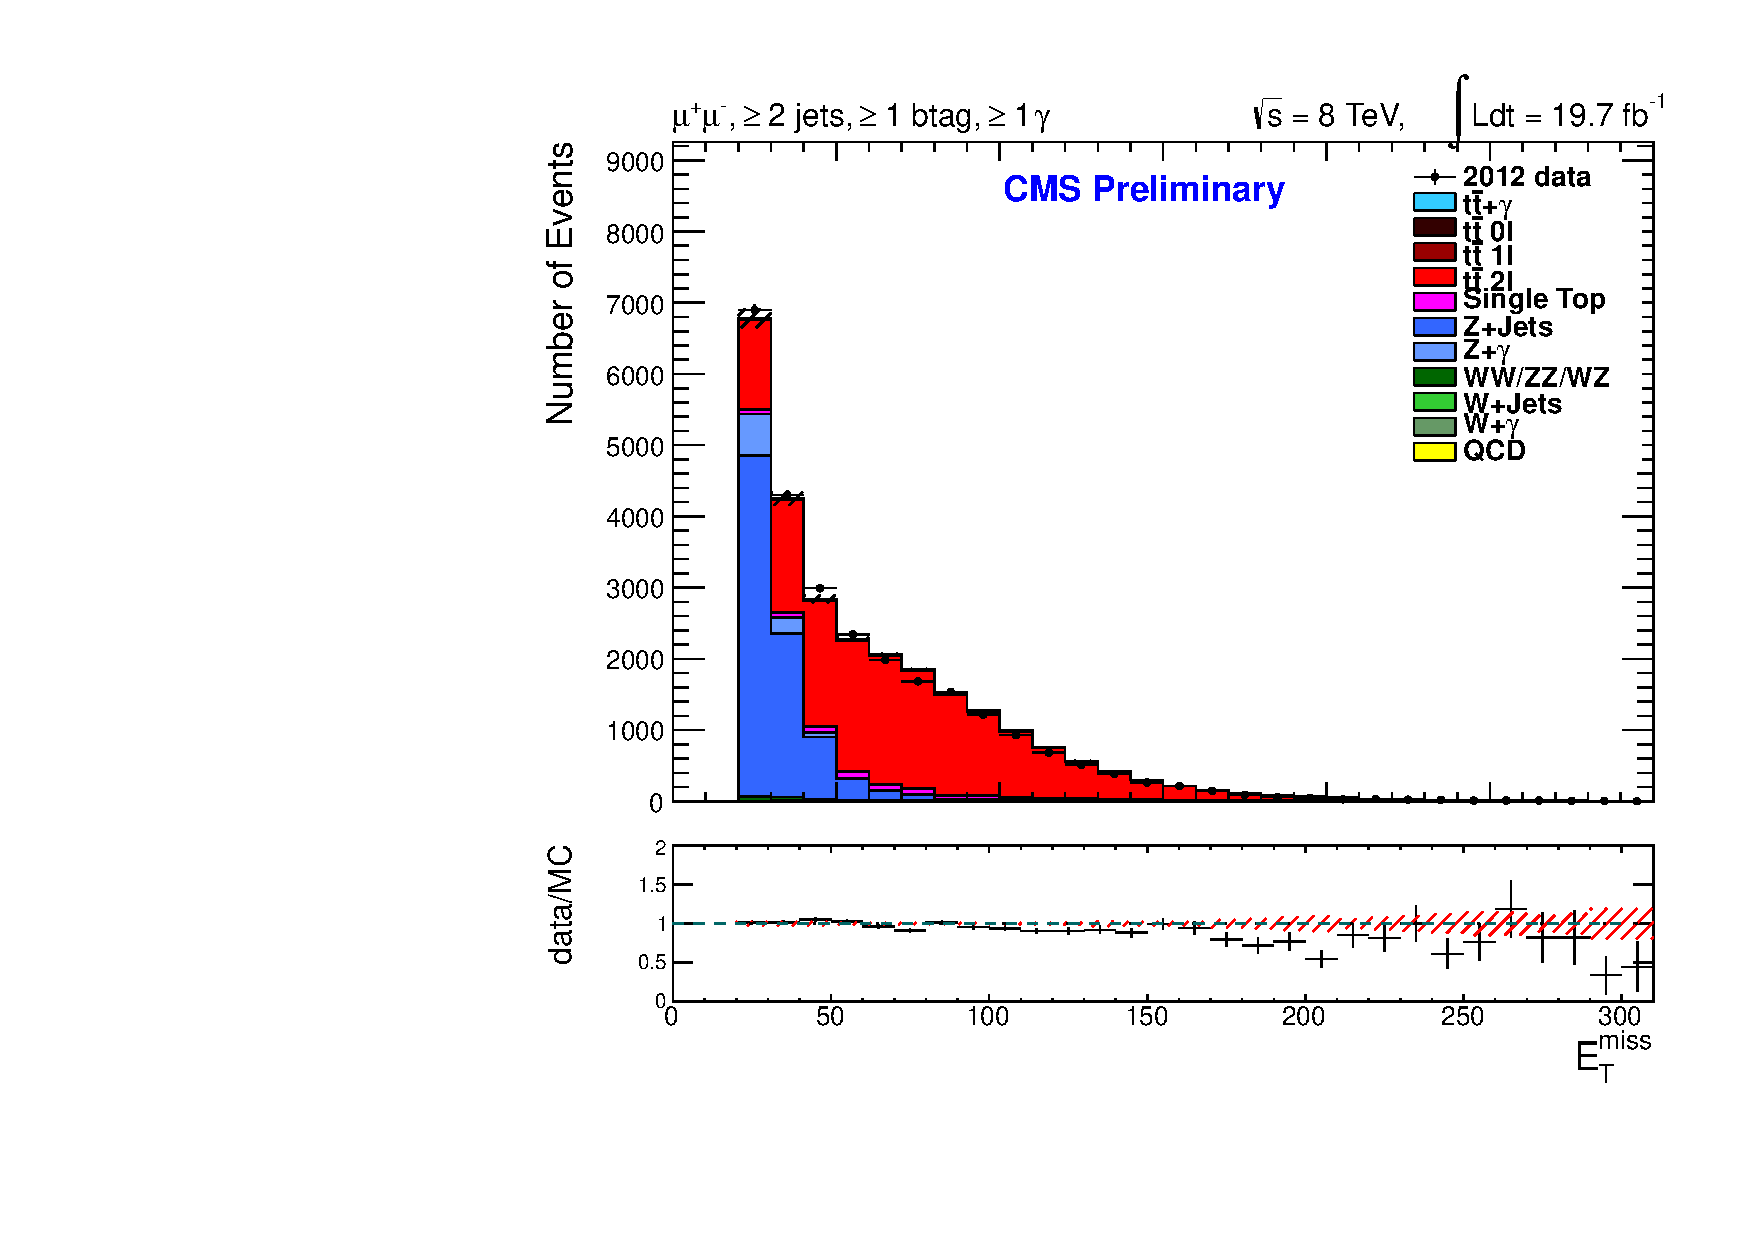
\includegraphics[width=0.5\textwidth]{Plots/ControlPlots/TTbarDiLeptonAnalysis/MuMu/MET/patType1CorrectedPFMet/MET_splitTTbar_ratio.pdf}
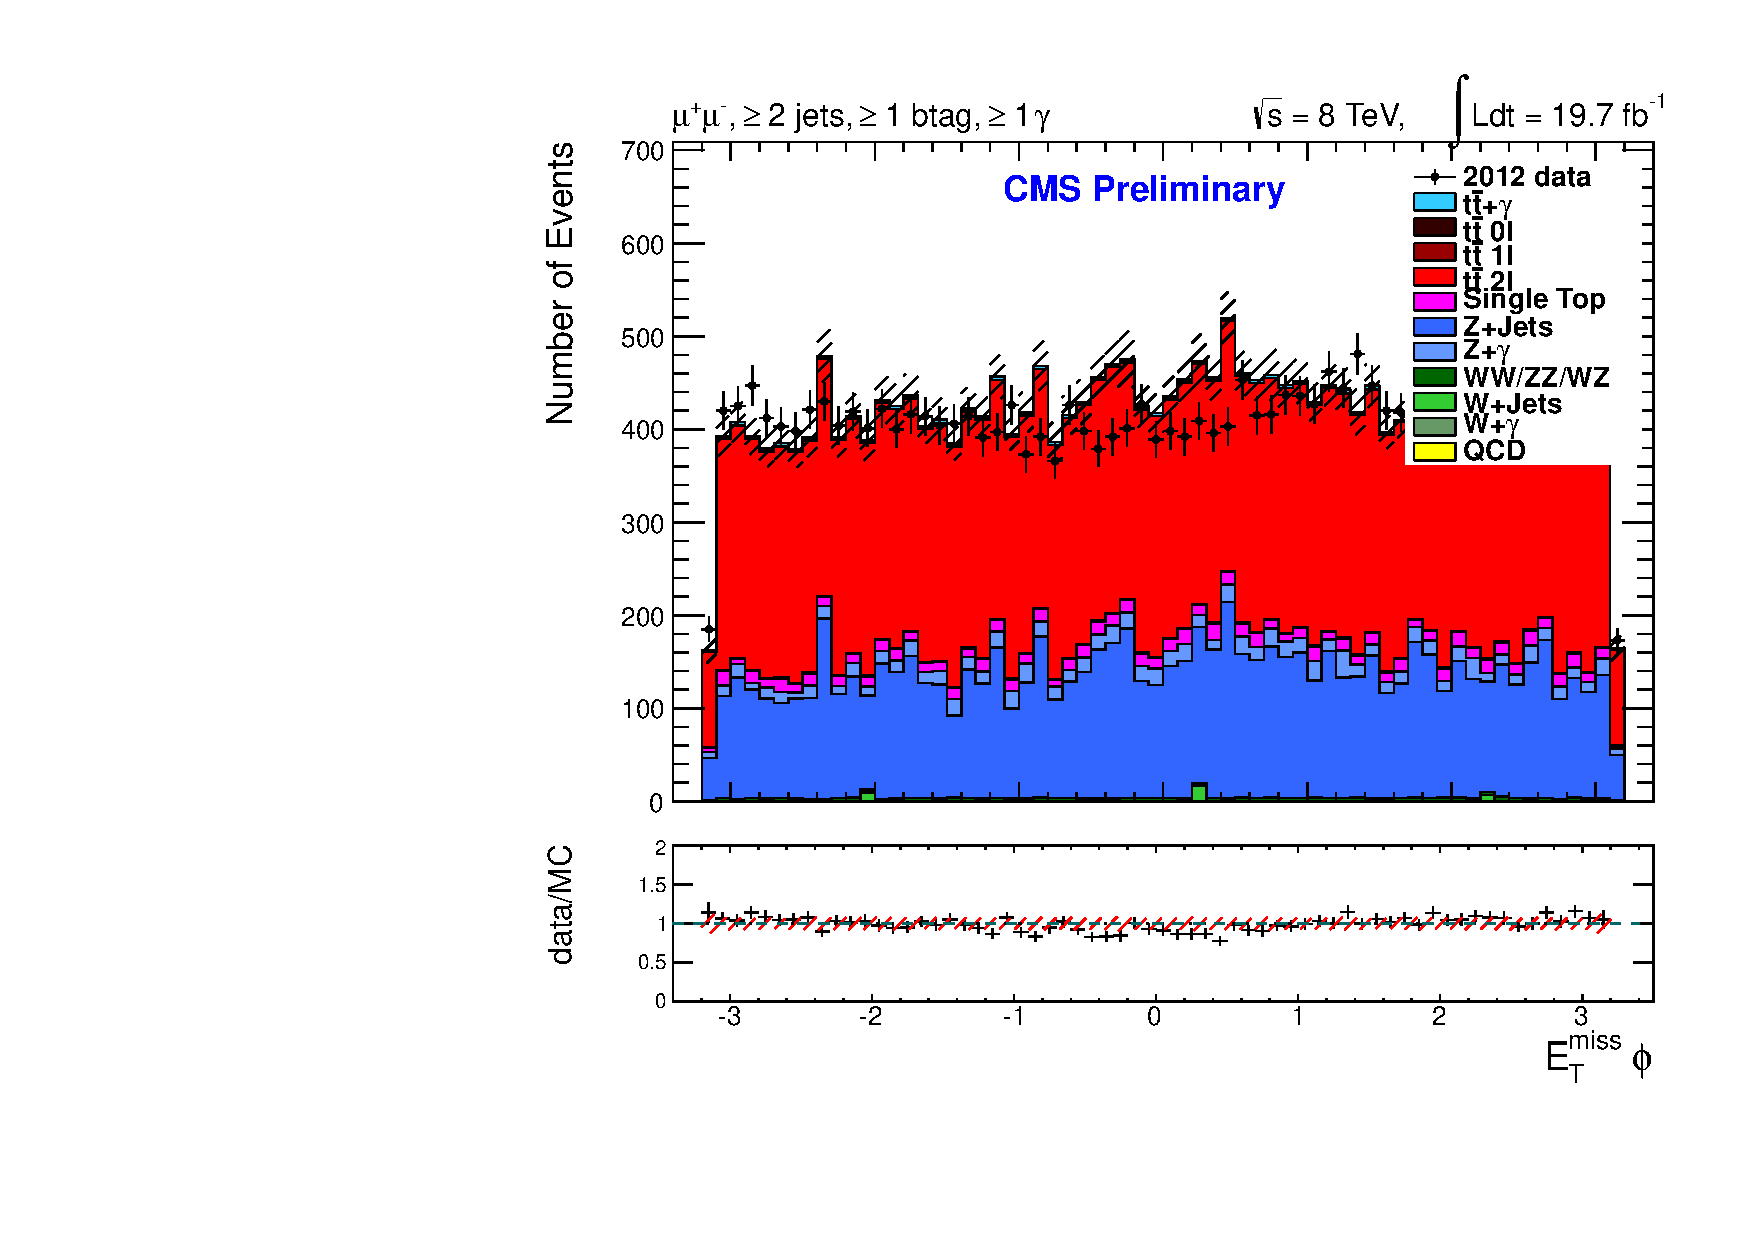
\includegraphics[width=0.5\textwidth]{Plots/ControlPlots/TTbarDiLeptonAnalysis/MuMu/MET/patType1CorrectedPFMet/MET_phi_splitTTbar_ratio.pdf}\\
\begin{center}
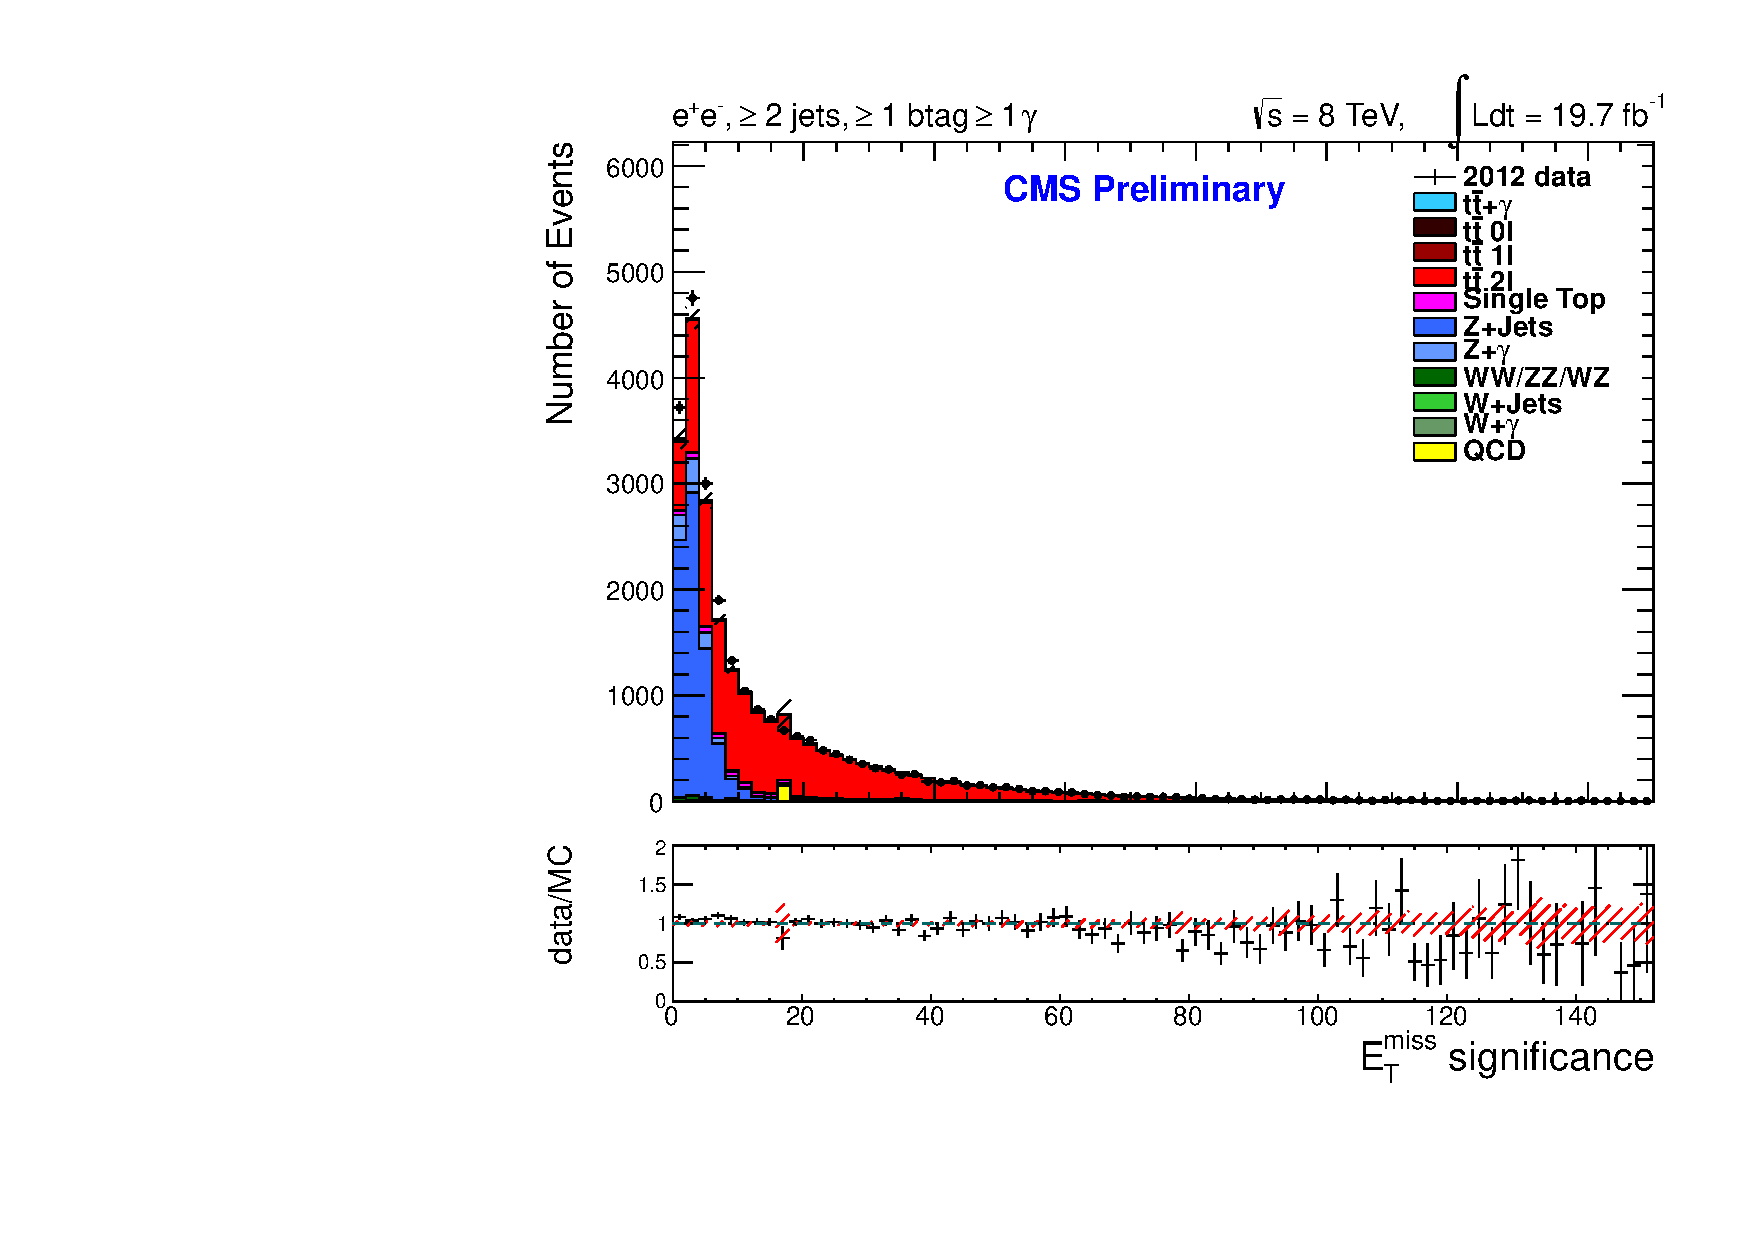
\includegraphics[width=0.5\textwidth]{Plots/ControlPlots/TTbarDiLeptonAnalysis/EE/MET/patType1CorrectedPFMet/METsignificance_splitTTbar_ratio.pdf}
\end{center}
\caption{The missing transverse energy distributions in terms of missing energy, azimuthal angle $\phi$, and MET significance for the $\mu^{+}\mu^{-}$ channel only after $t\bar{t}$ selection.}
\label{fig-METphiSig}
\end{figure}

\section{Comparison of data and simulation for $t\bar{t}$ selection}

After implementing all of the aforementioned selection requirements for $t\bar{t}$ events, a comparison of the events from data and from simulation can be conducted in order to test the agreement between the two. Figure \ref{fig-ttbarETandEta} shows the photon transverse energy and absolute pseudorapidity for each of the decay channels, and it can be seen that, after all selection requirements have been introduced in both data and simulation, there is good agreement between data and simulation. 

\begin{figure}
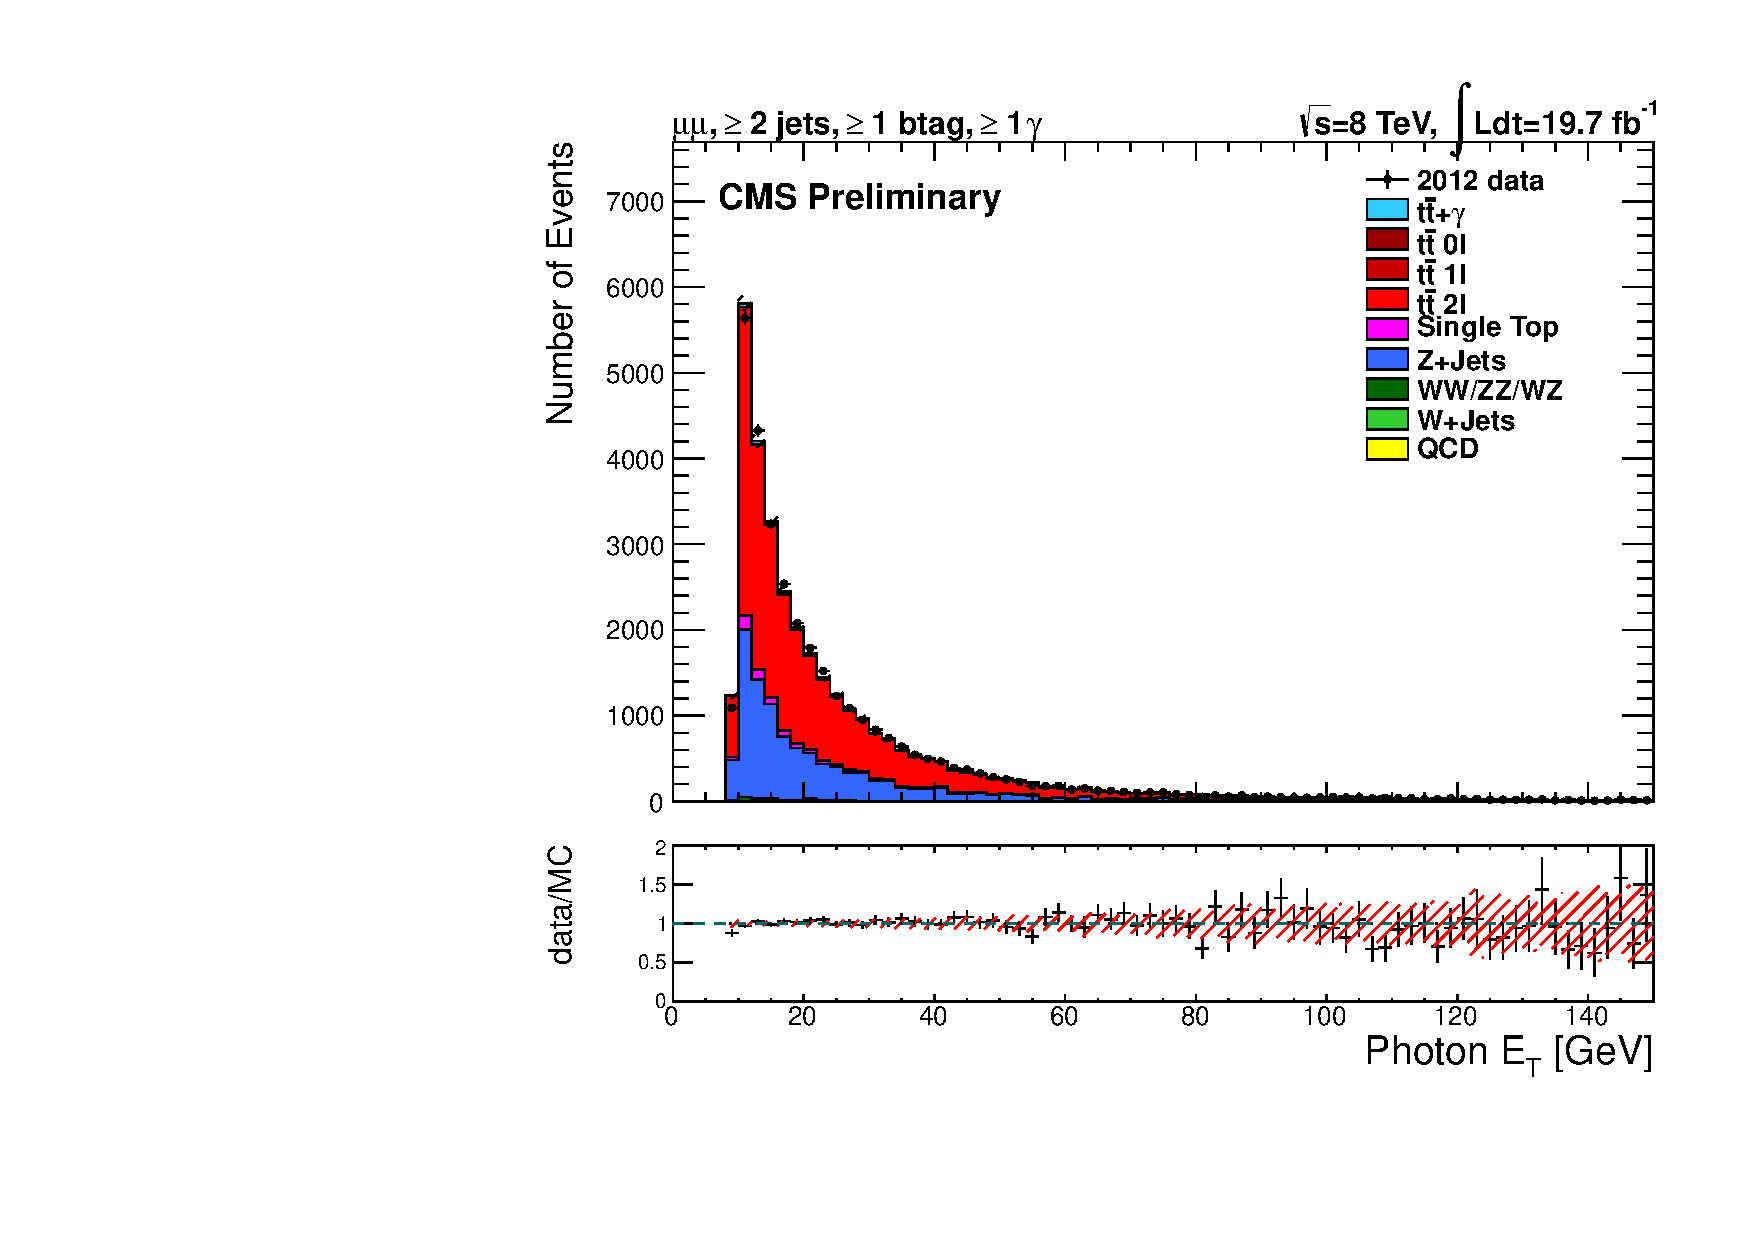
\includegraphics[width=0.5\textwidth]{Plots/ControlPlots/TTbarDiLeptonAnalysis/MuMu/Photons/AllPhotons/Photon_ET_splitTTbar_ratio.pdf}
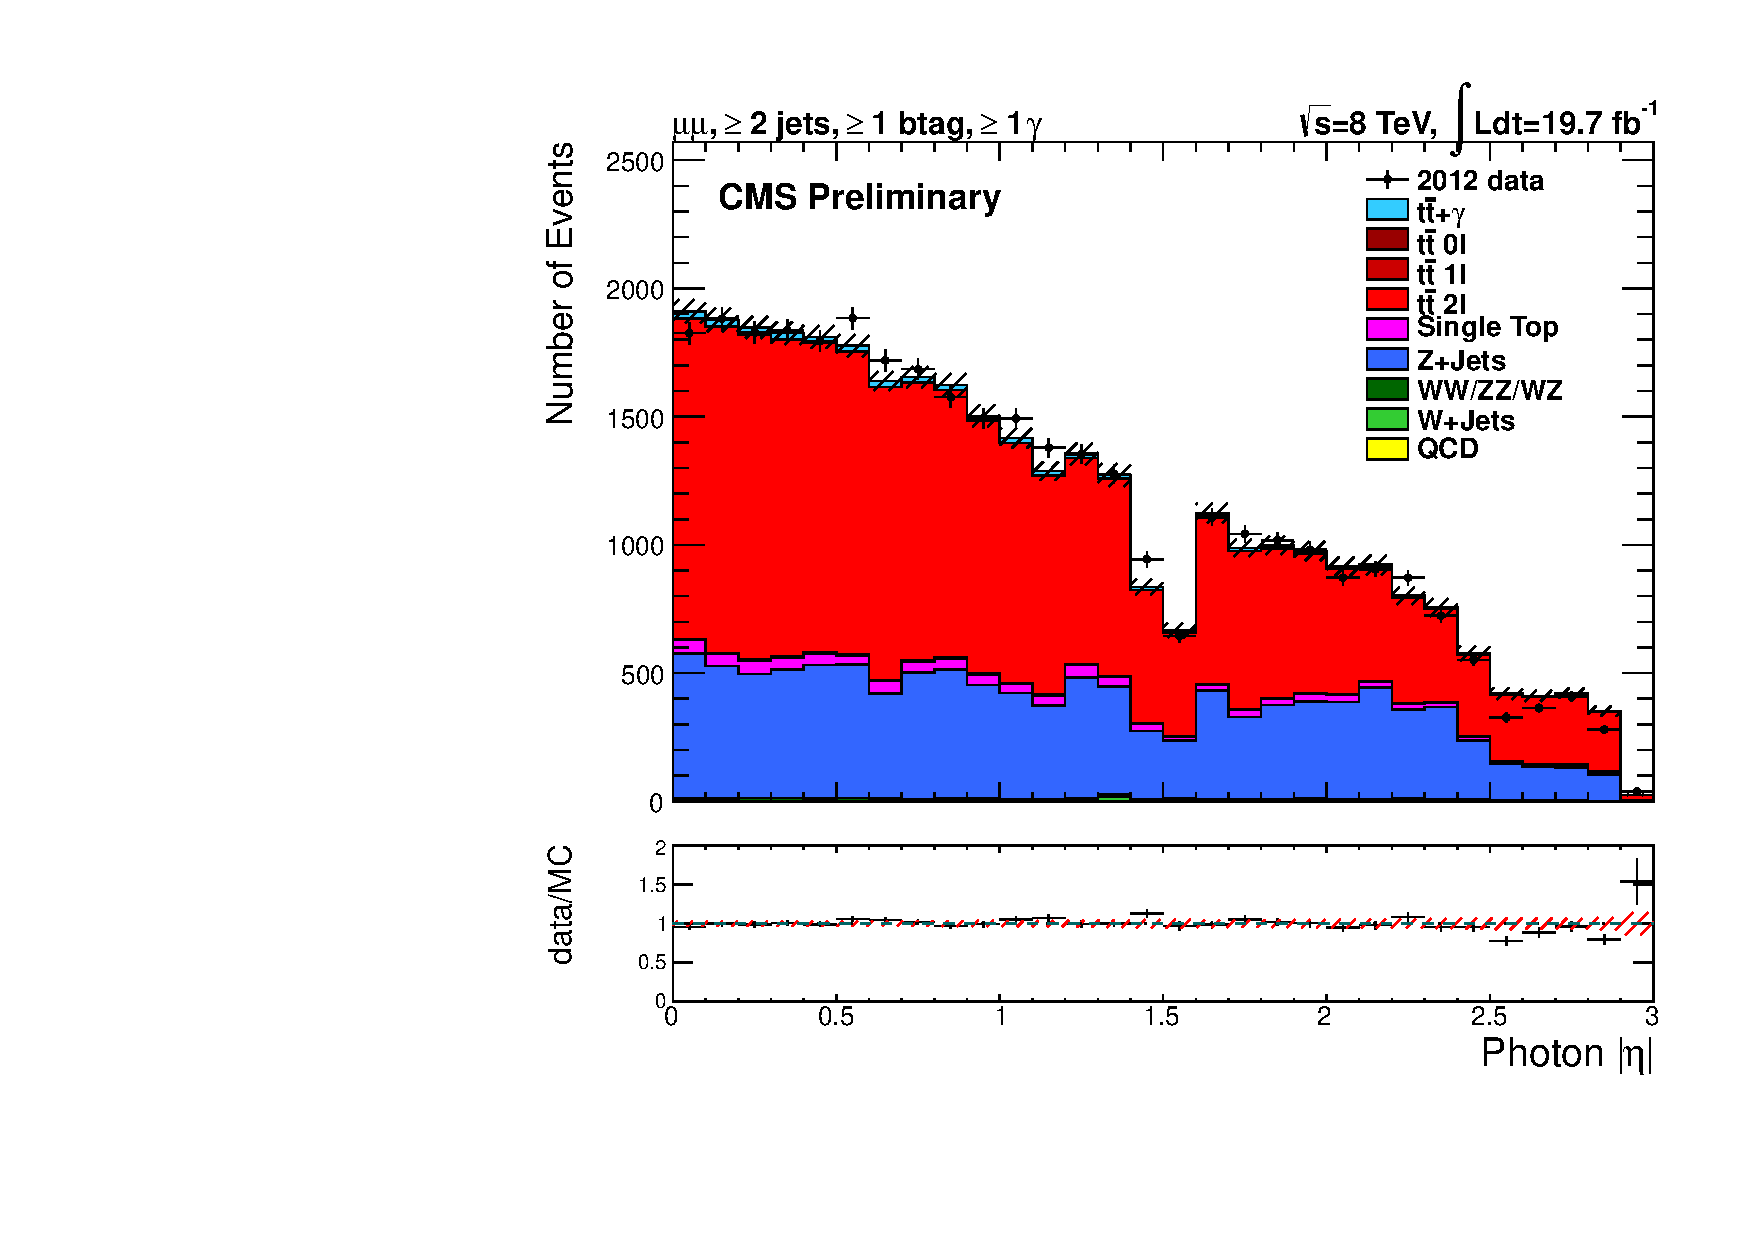
\includegraphics[width=0.5\textwidth]{Plots/ControlPlots/TTbarDiLeptonAnalysis/MuMu/Photons/AllPhotons/Photon_AbsEta_splitTTbar_ratio.pdf}\\
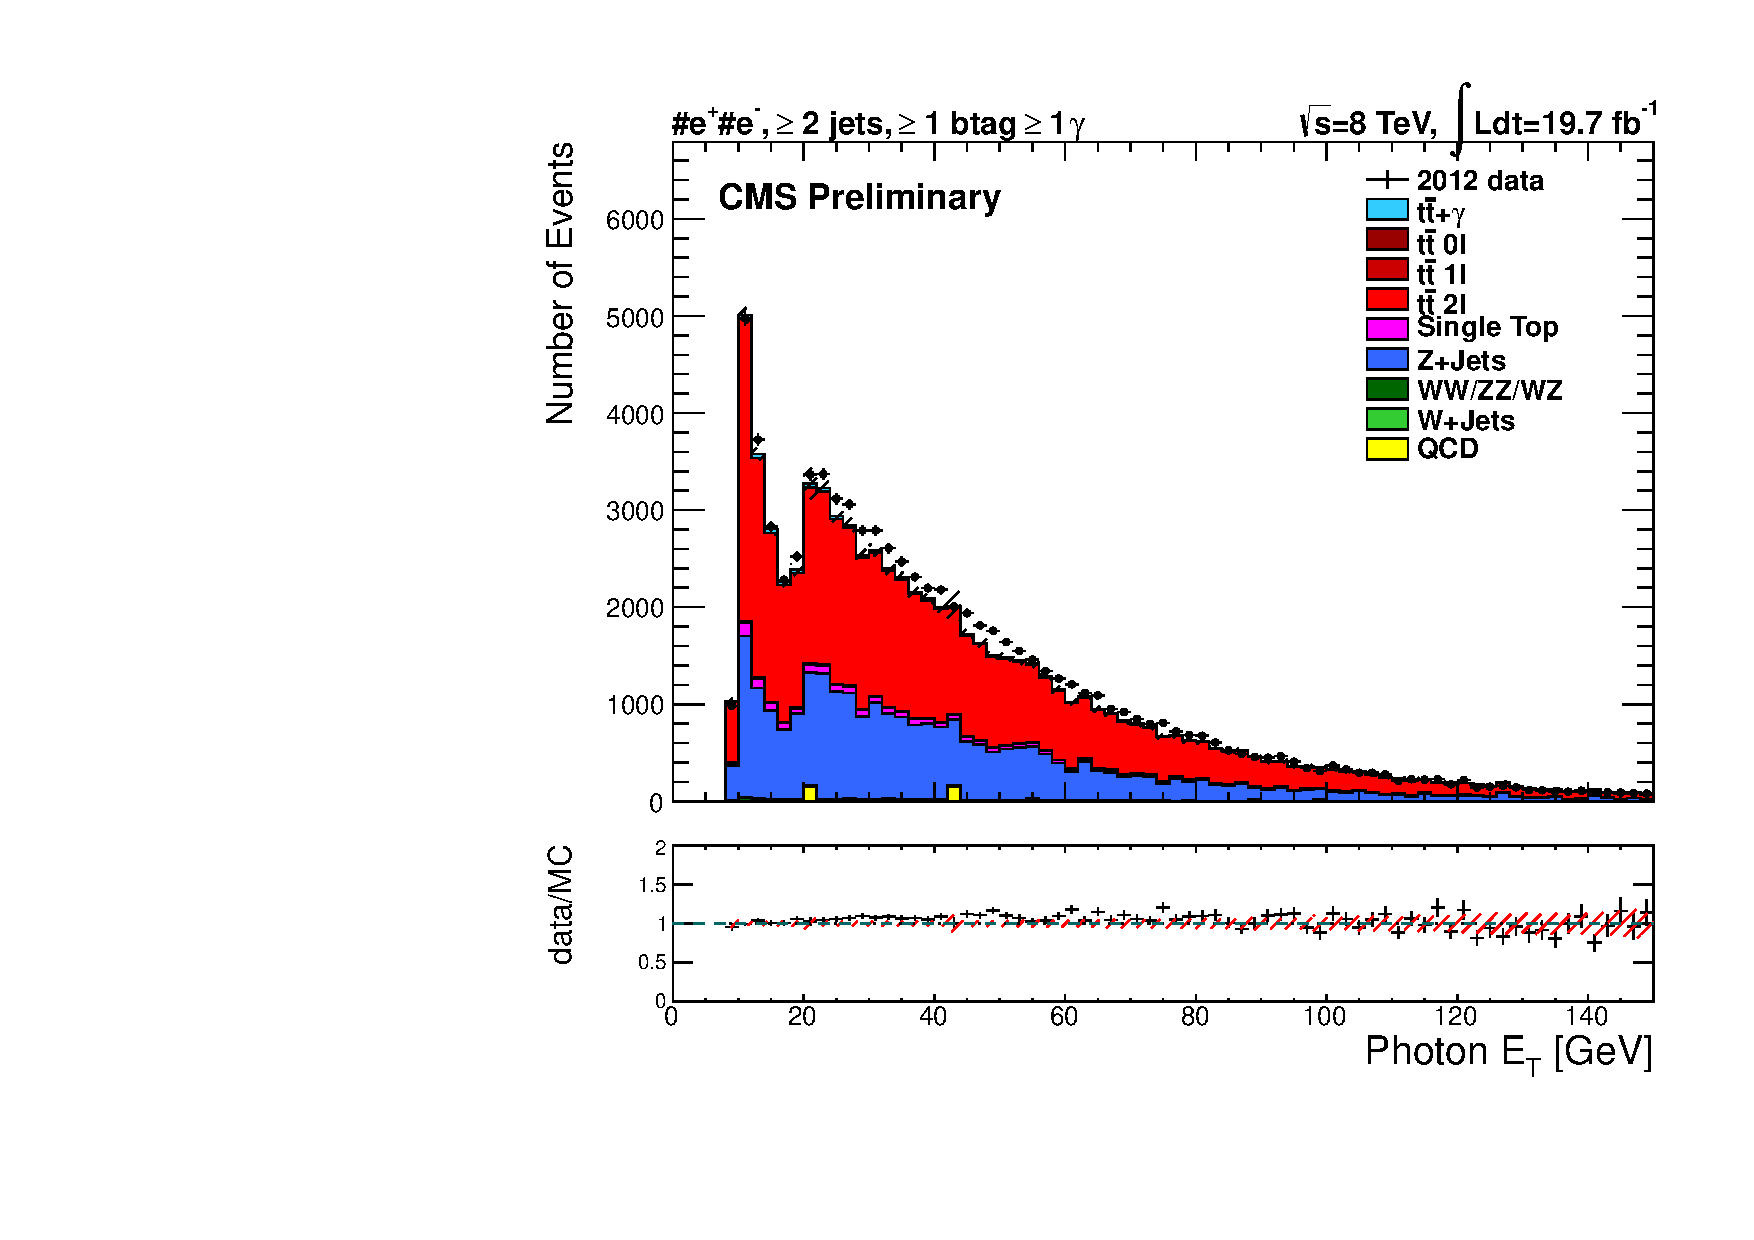
\includegraphics[width=0.5\textwidth]{Plots/ControlPlots/TTbarDiLeptonAnalysis/EE/Photons/AllPhotons/Photon_ET_splitTTbar_ratio.pdf}
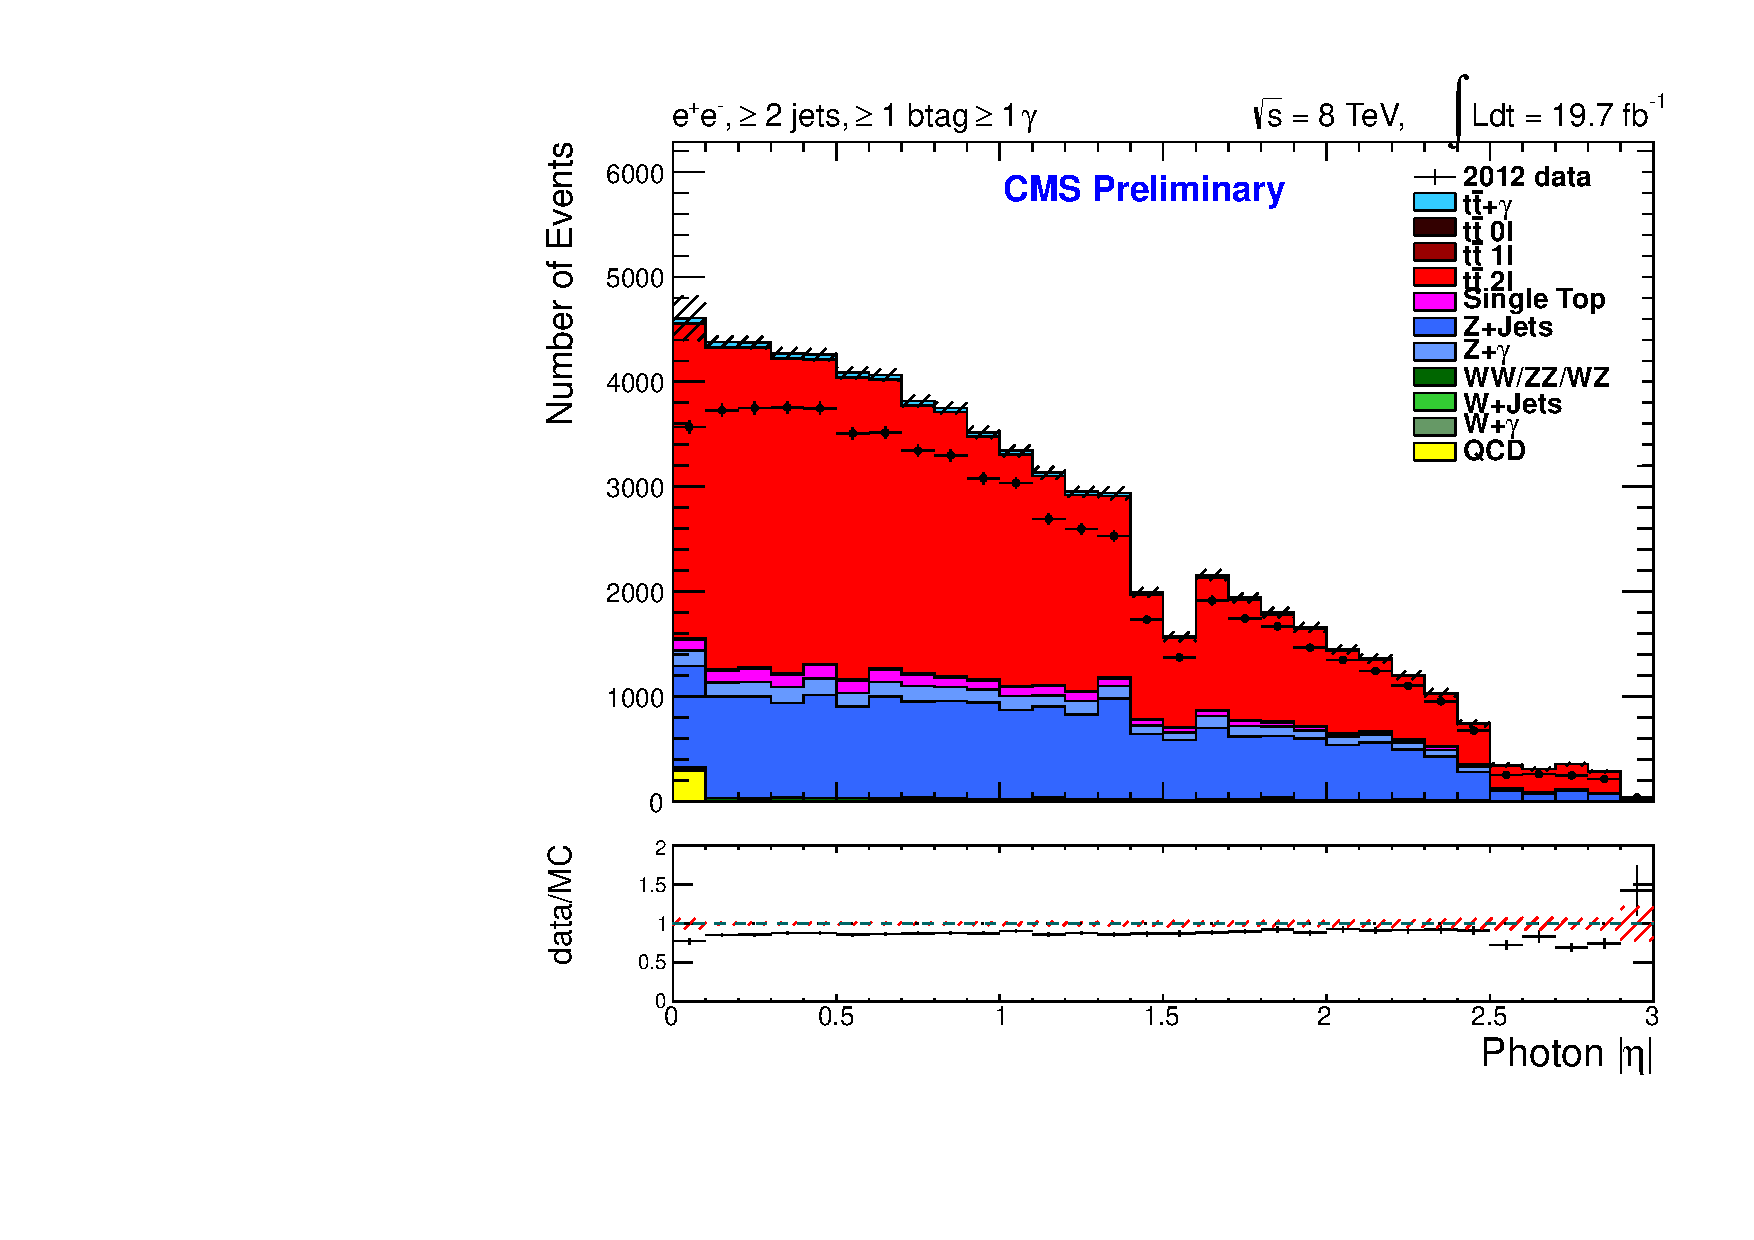
\includegraphics[width=0.5\textwidth]{Plots/ControlPlots/TTbarDiLeptonAnalysis/EE/Photons/AllPhotons/Photon_AbsEta_splitTTbar_ratio.pdf}\\
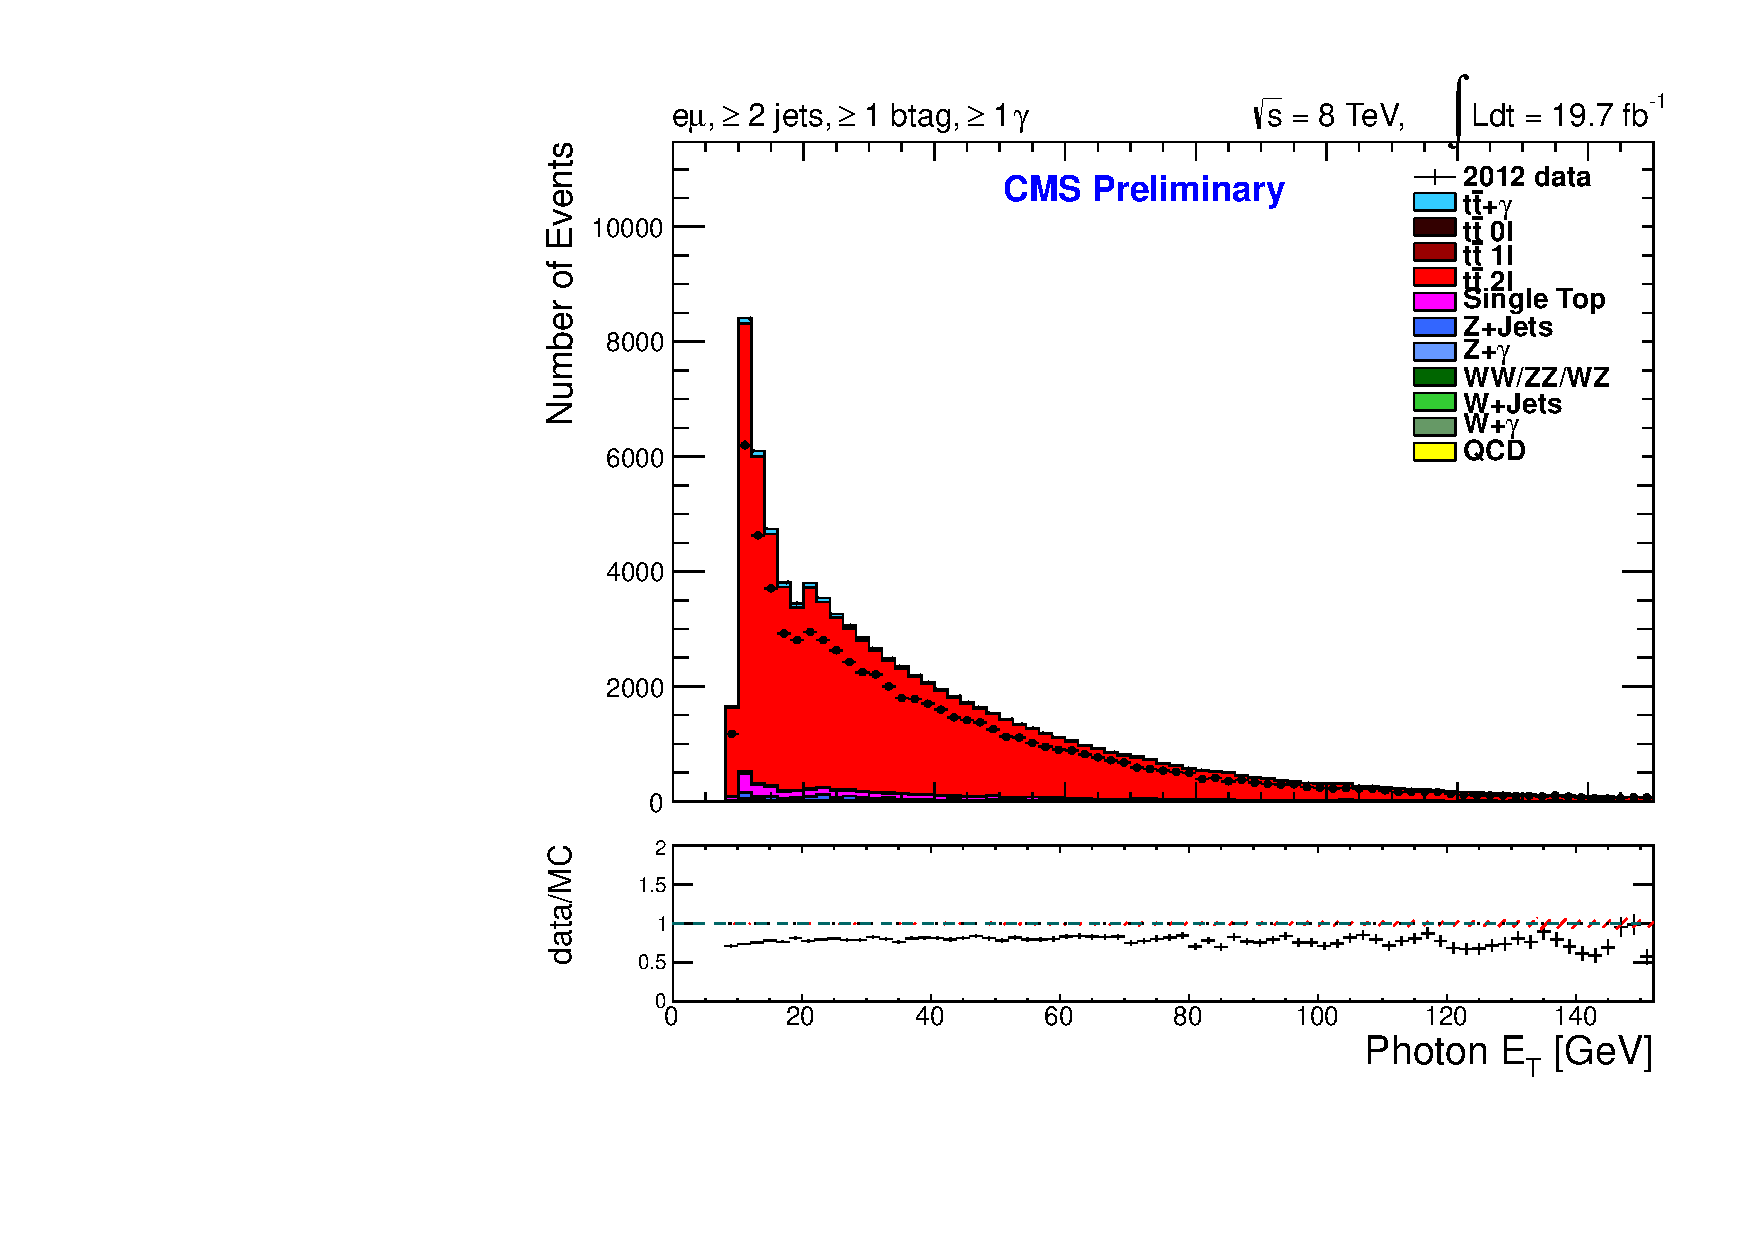
\includegraphics[width=0.5\textwidth]{Plots/ControlPlots/TTbarDiLeptonAnalysis/EMu/Photons/AllPhotons/Photon_ET_splitTTbar_ratio.pdf}
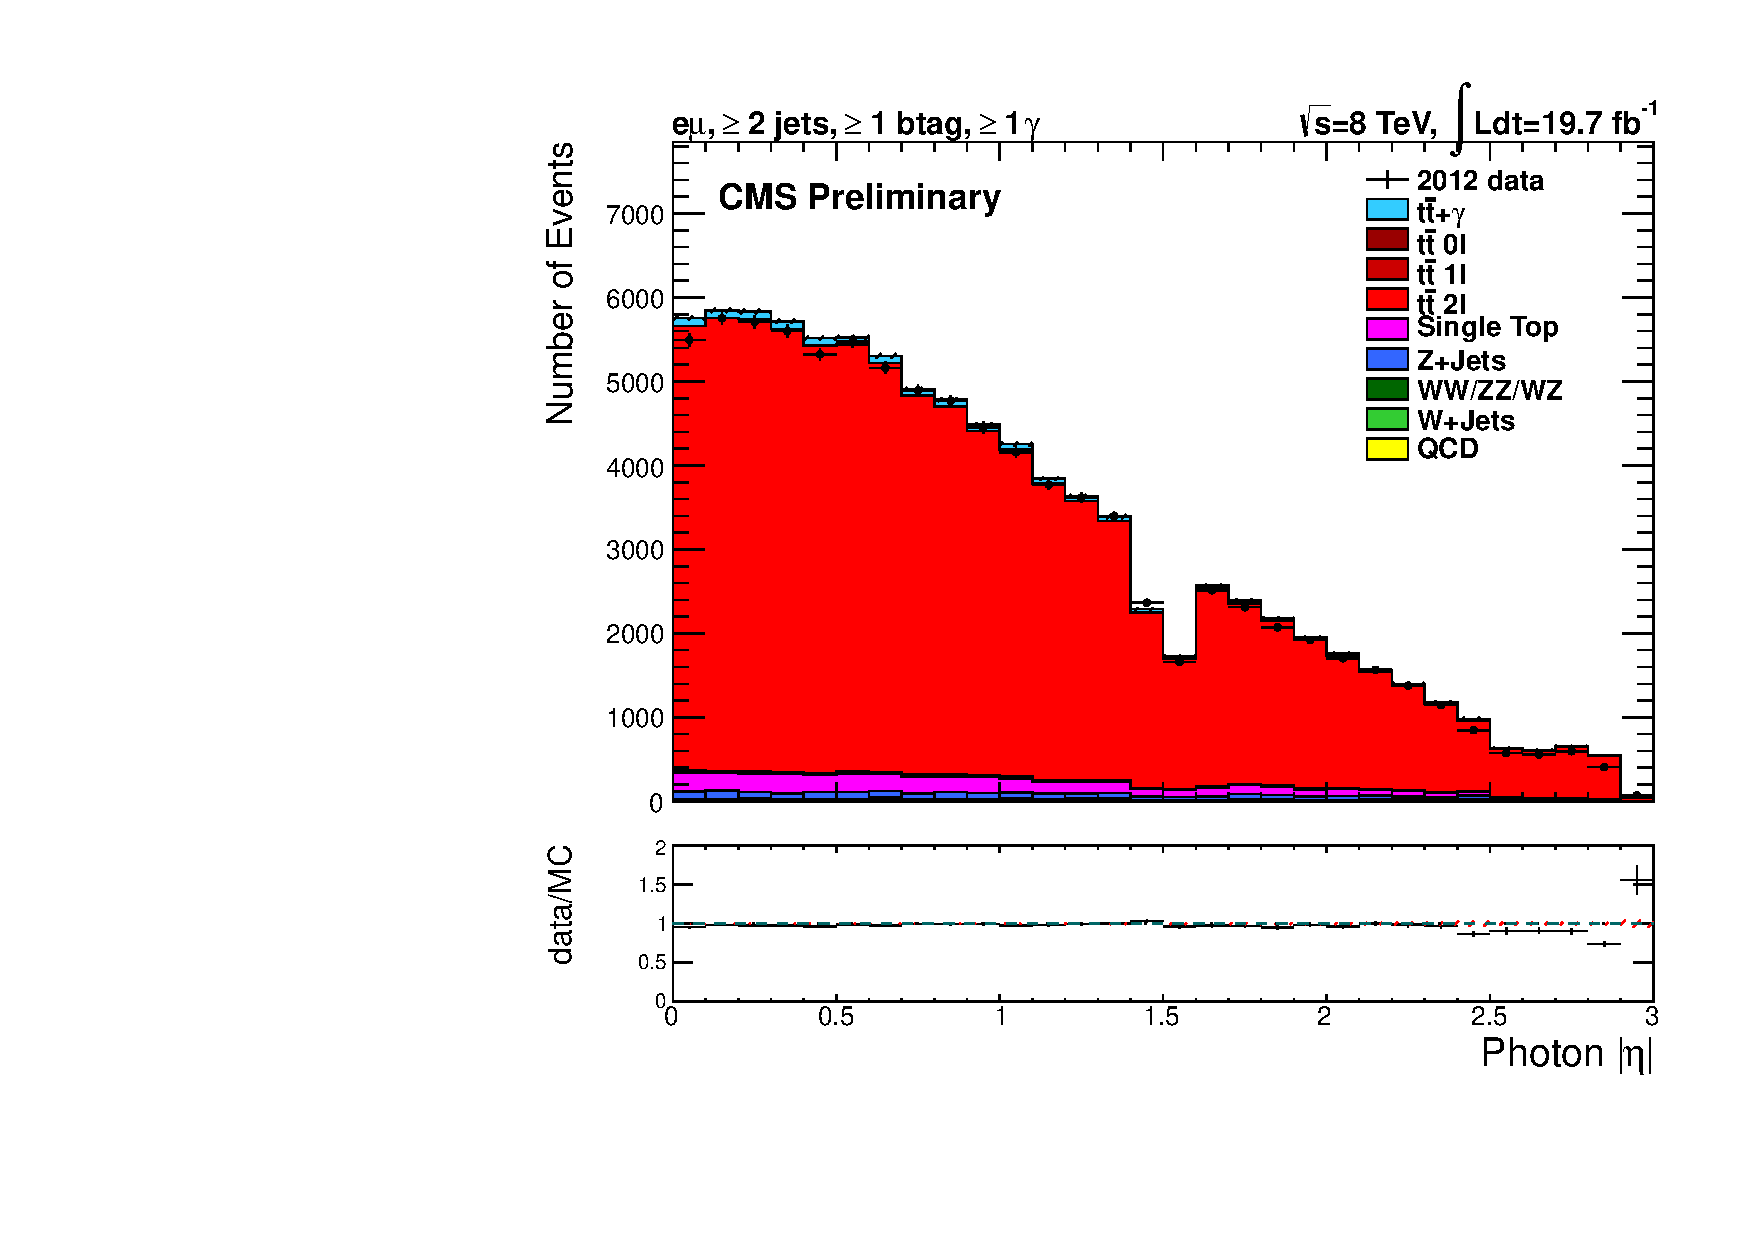
\includegraphics[width=0.5\textwidth]{Plots/ControlPlots/TTbarDiLeptonAnalysis/EMu/Photons/AllPhotons/Photon_AbsEta_splitTTbar_ratio.pdf}
\caption{Comparison of the photon E$_{T}$ and $|\eta|$ distributions in data and simulation in the $\mu^{+}\mu^{-}$, $e^{+}e^{-}$, and $e\mu$ channels after $t\bar{t}$ selection.}
\label{fig-ttbarETandEta}
\end{figure}

\section{Selection of $t\bar{t}+\gamma$ events} \label{sec-postselection}

From the set of $t\bar{t}$ preselected events in Section \ref{sec-preselection}, only events with a photon candidate present are selected.  Fiducial requirements are implemented in both $\abs{\eta}$ and $E_T$. CMS recommended selection requirements are implemented and photon selection (loose cut-based photon ID 2012 with particle flow-based isolation, \cite{CutBasedIsolation2012}).In order to suppress Final State Radiation (FSR), a $\Delta R$ requirement for photons between jets and leptons is applied.

The fiducial cuts on the photon are given as follows:

\begin{description}

\item[Transverse energy] A transverse energy cut of $E_T > 25$ GeV is implemented in order to suppress the numerous low energy fake photons and photons from vertices other than the primary vertex. The transverse energy distribution for each decay channel can be seen in Figure \ref{fig-photonSelectionETandEta}, where we observe a good agreement between data and MC.

\item[Pseudorapidity] An acceptance cut on the fiducial region of just the CMS ECAL barrel (EB), $\abs{\eta} < 1.4442$, is applied to ensure that the electromagnetic shower of the photon will be fully reconstructed. The ECAL Endcap (EE) is not included in this analysis due to the difficulty in identifying a photon in this region.

\end{description}

The fiducial variable distributions are shown in Figure \ref{fig-photonSelectionETandEta}.

\begin{figure}
% \begin{center}
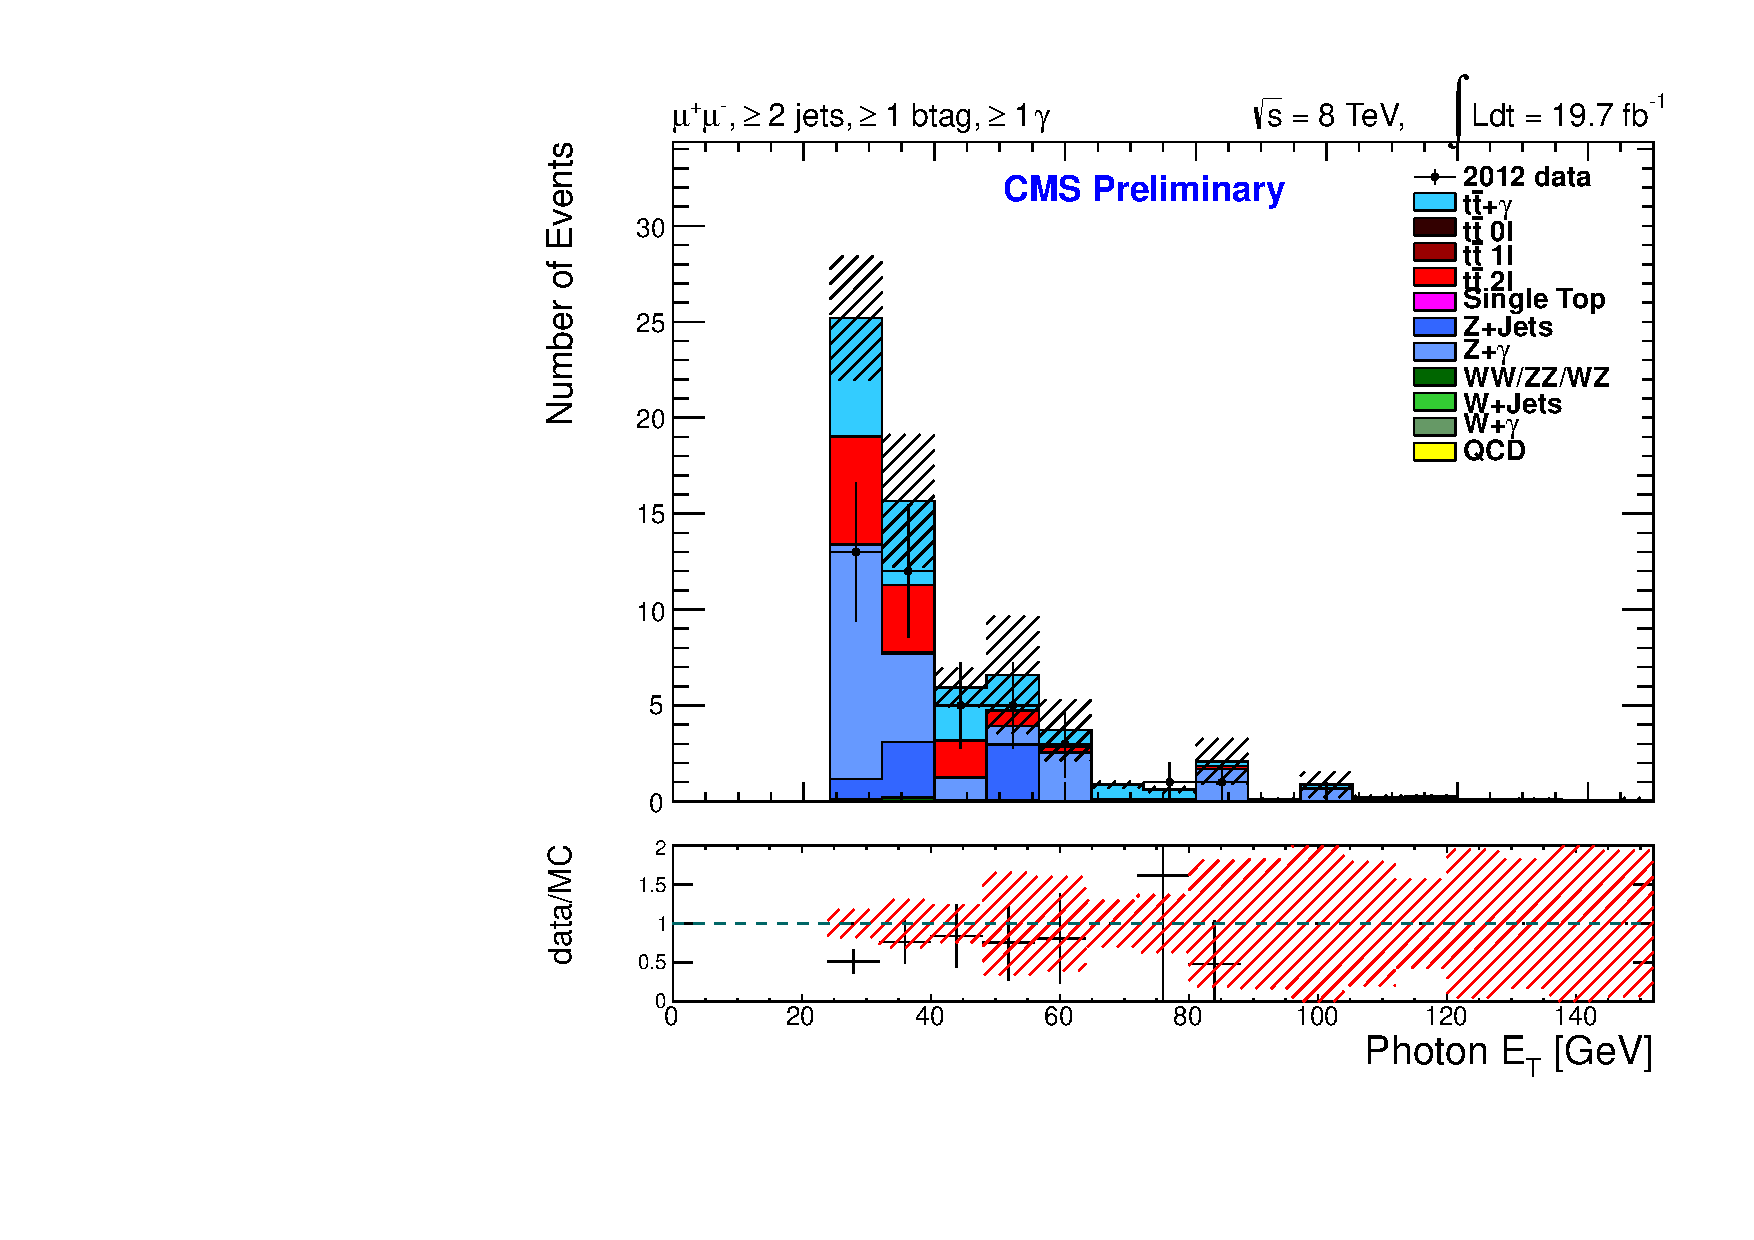
\includegraphics[width=0.5\textwidth]{Plots/ControlPlots/TTbarPhotonAnalysis/MuMu/Photons/SignalPhotons/Photon_ET_splitTTbar_ratio.pdf}
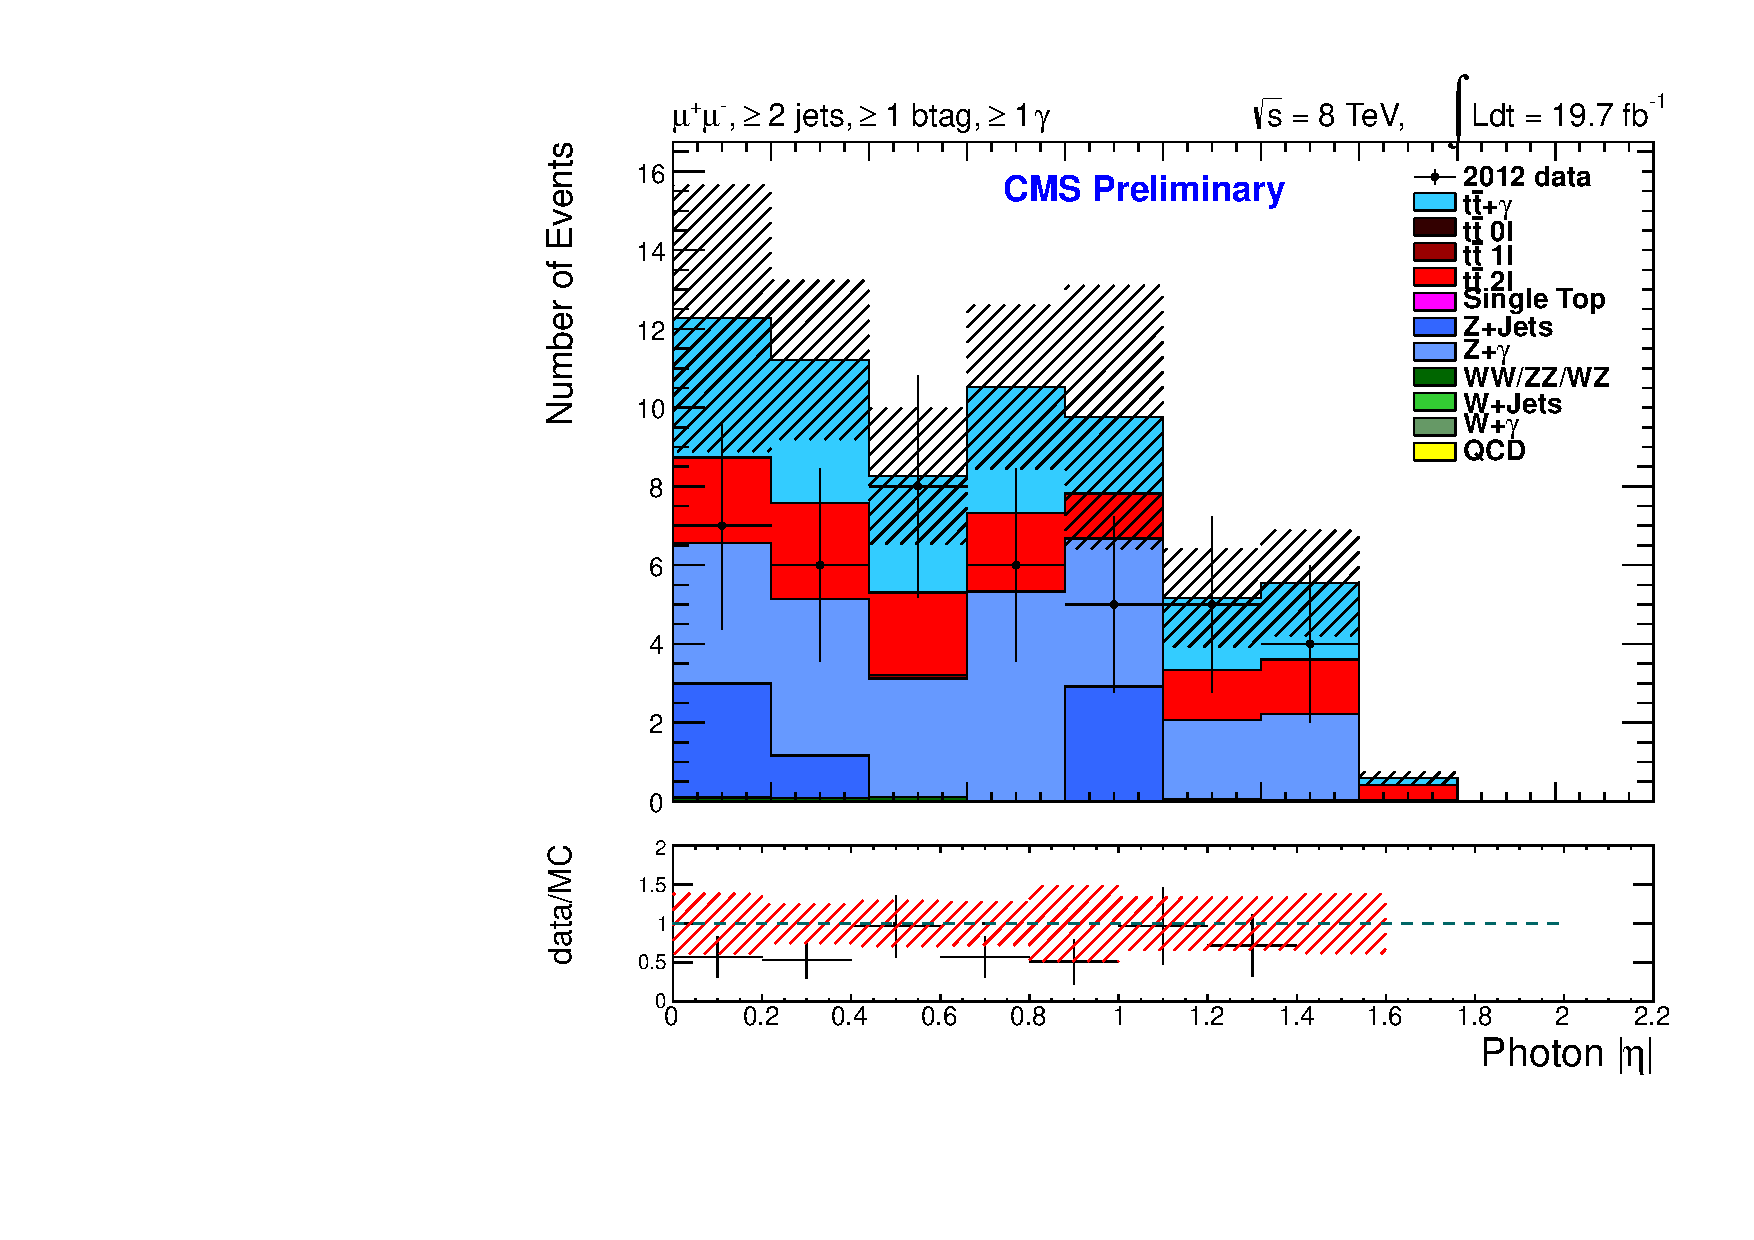
\includegraphics[width=0.5\textwidth]{Plots/ControlPlots/TTbarPhotonAnalysis/MuMu/Photons/SignalPhotons/Photon_AbsEta_splitTTbar_ratio.pdf} \\
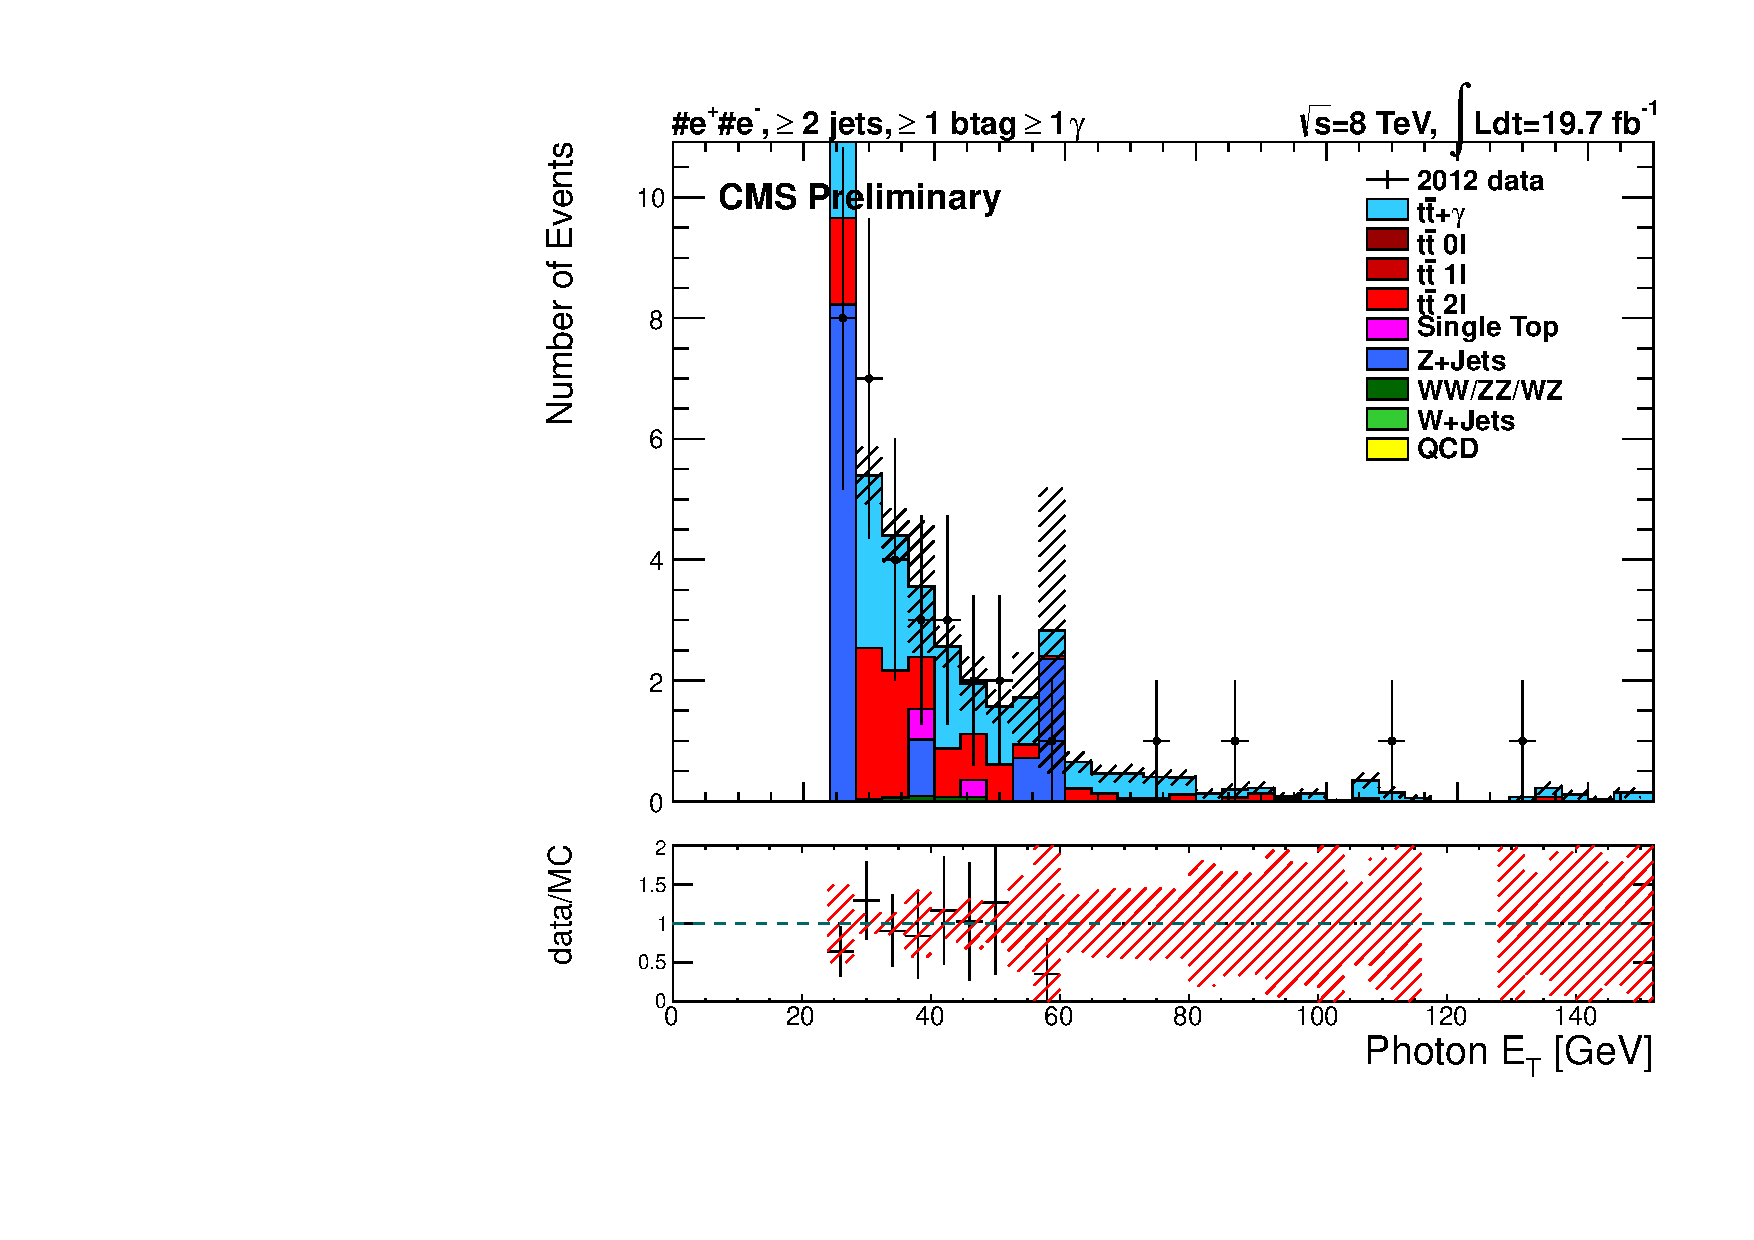
\includegraphics[width=0.5\textwidth]{Plots/ControlPlots/TTbarPhotonAnalysis/EE/Photons/SignalPhotons/Photon_ET_splitTTbar_ratio.pdf}
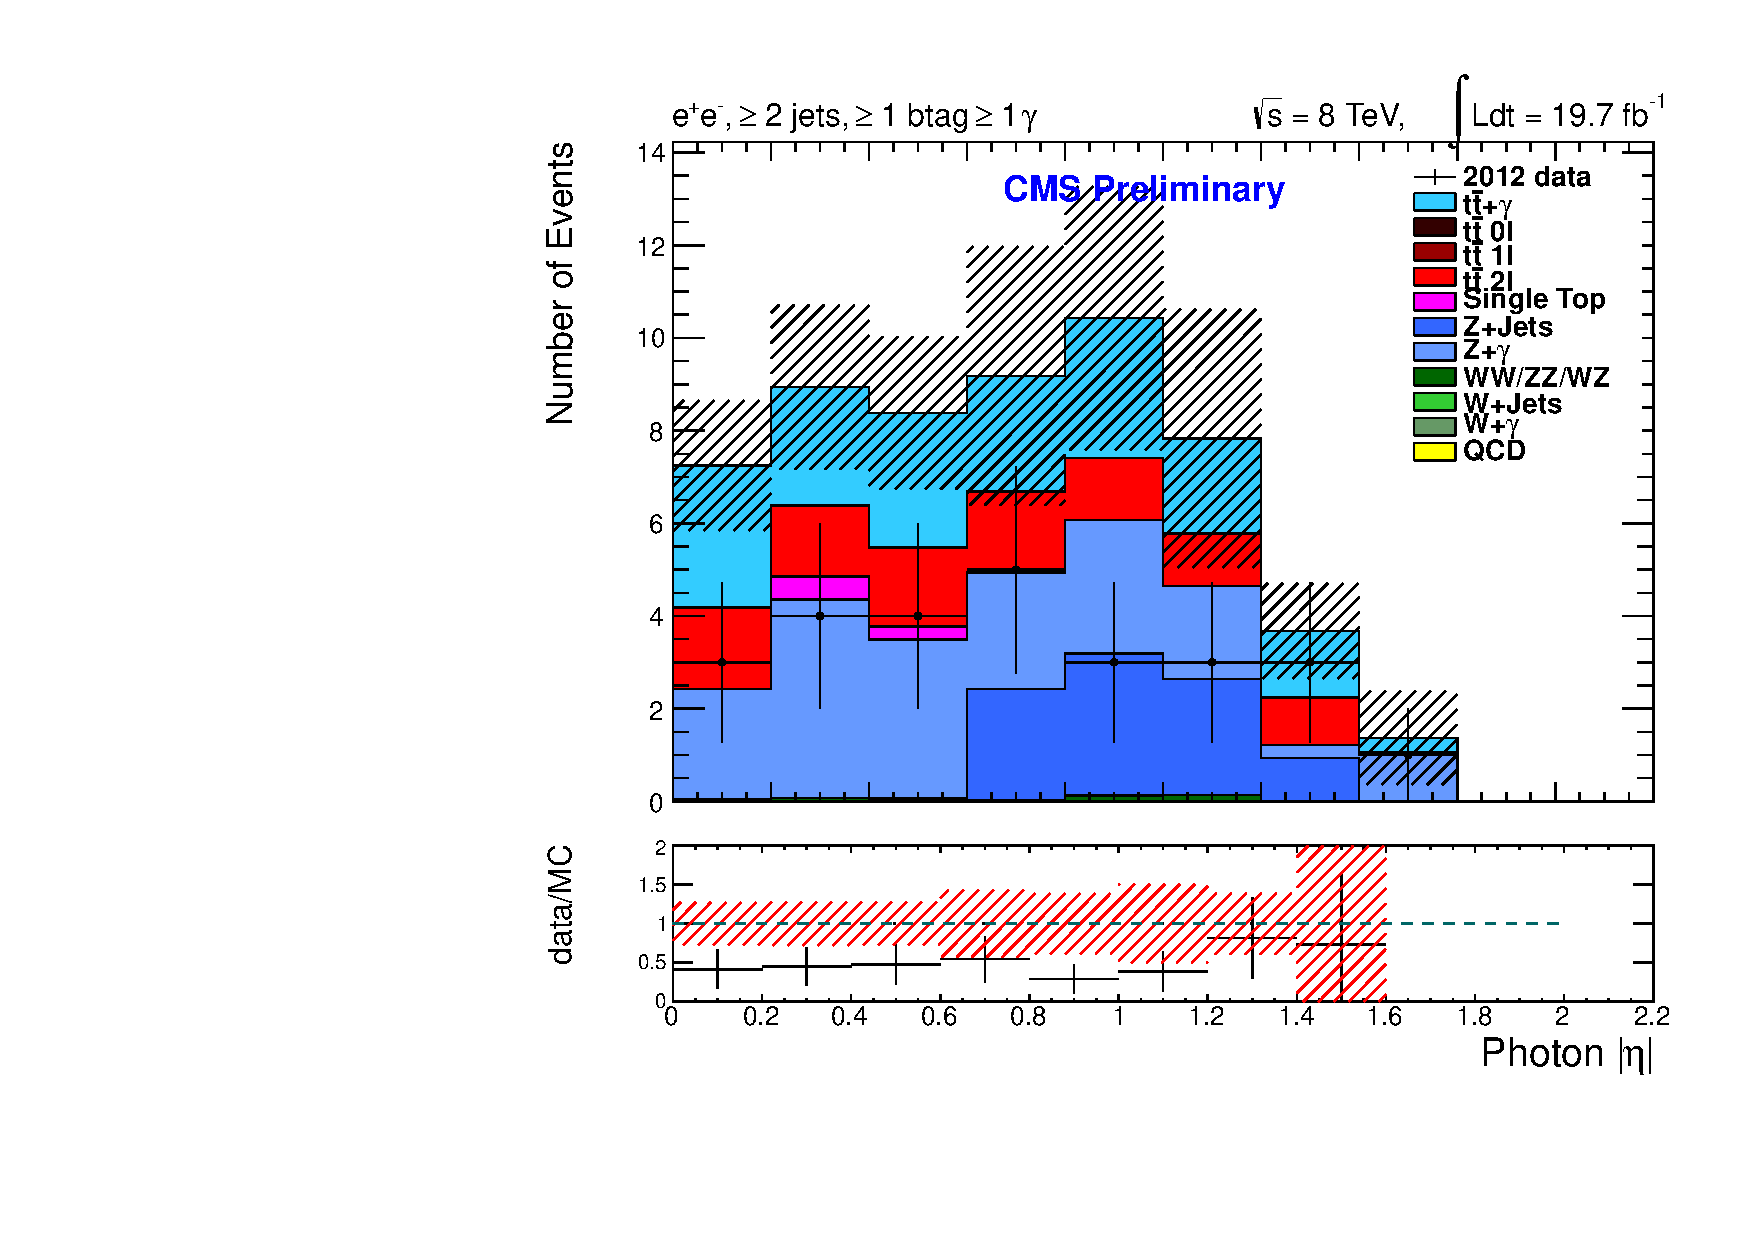
\includegraphics[width=0.5\textwidth]{Plots/ControlPlots/TTbarPhotonAnalysis/EE/Photons/SignalPhotons/Photon_AbsEta_splitTTbar_ratio.pdf} \\
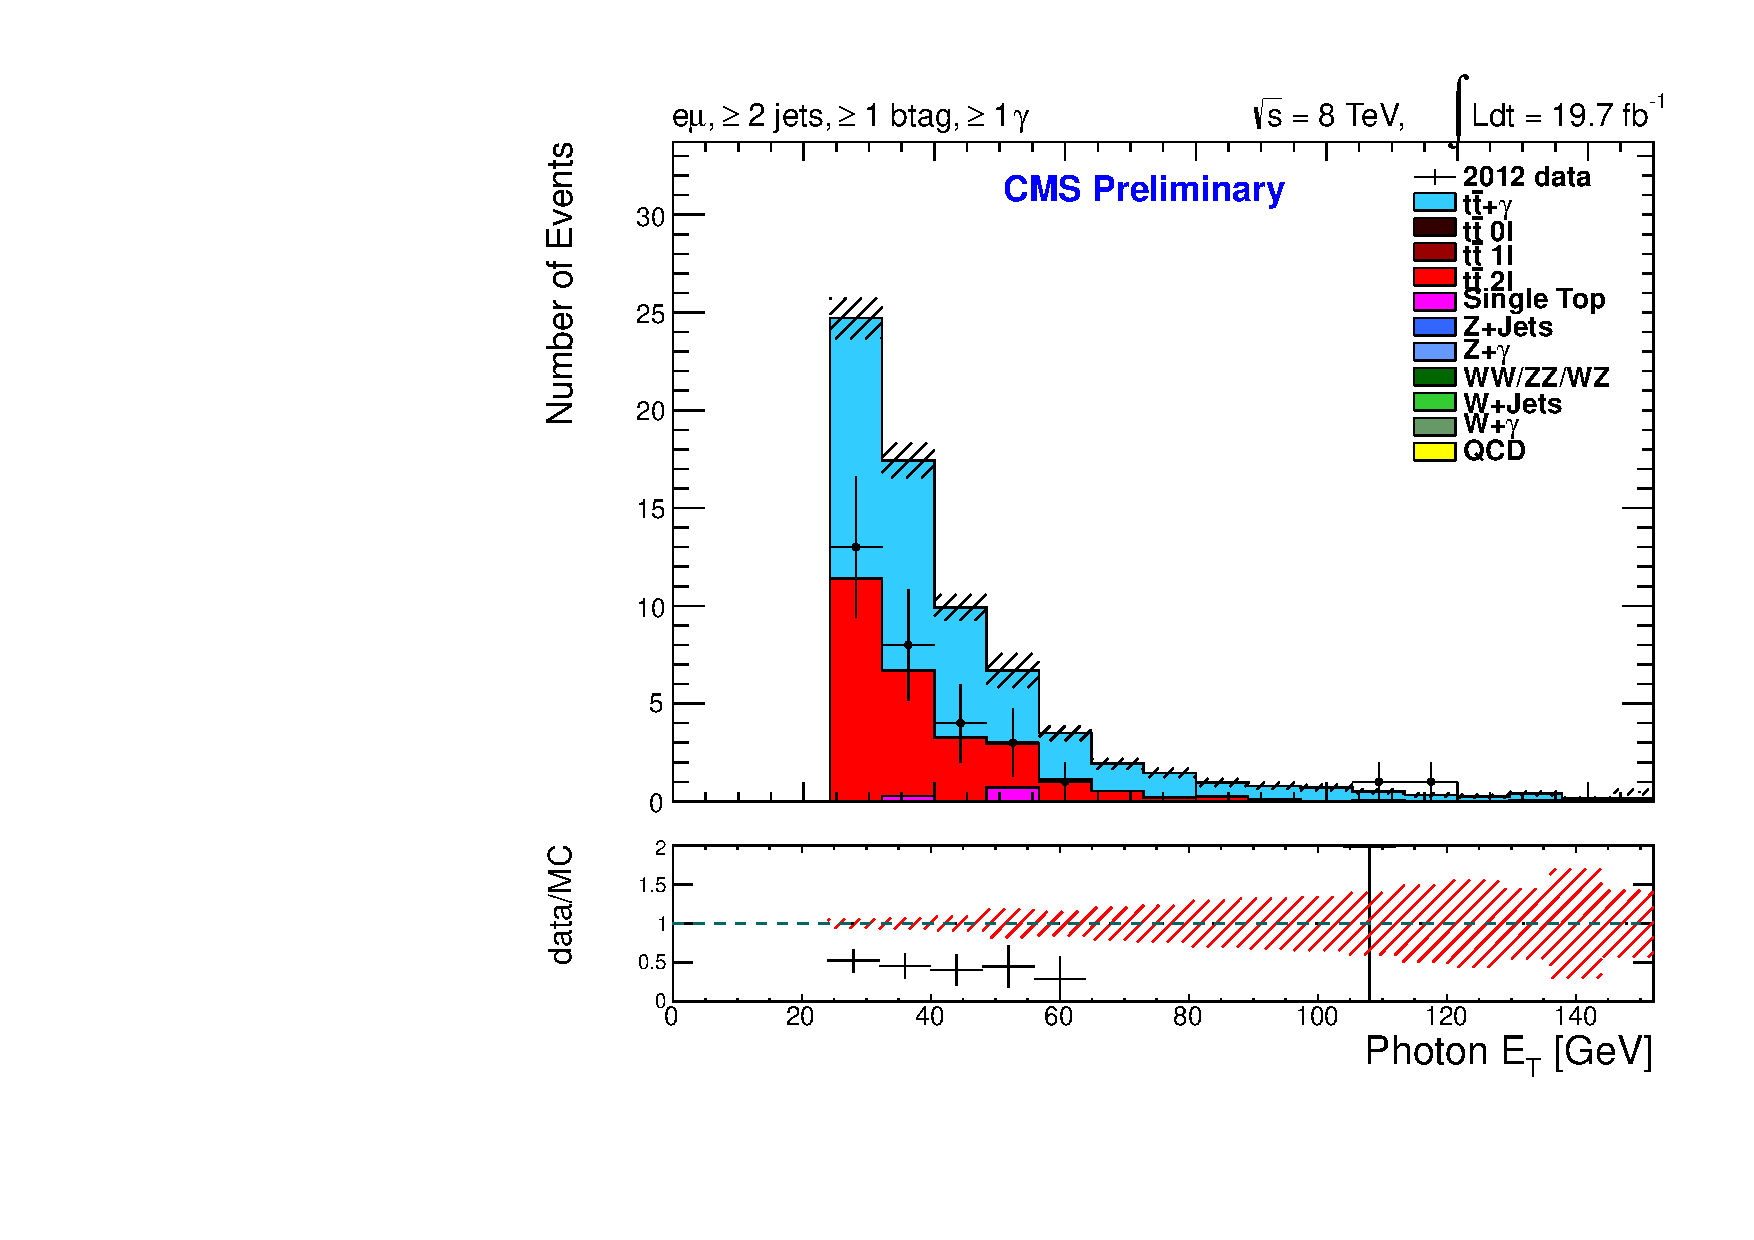
\includegraphics[width=0.5\textwidth]{Plots/ControlPlots/TTbarPhotonAnalysis/EMu/Photons/SignalPhotons/Photon_ET_splitTTbar_ratio.pdf}
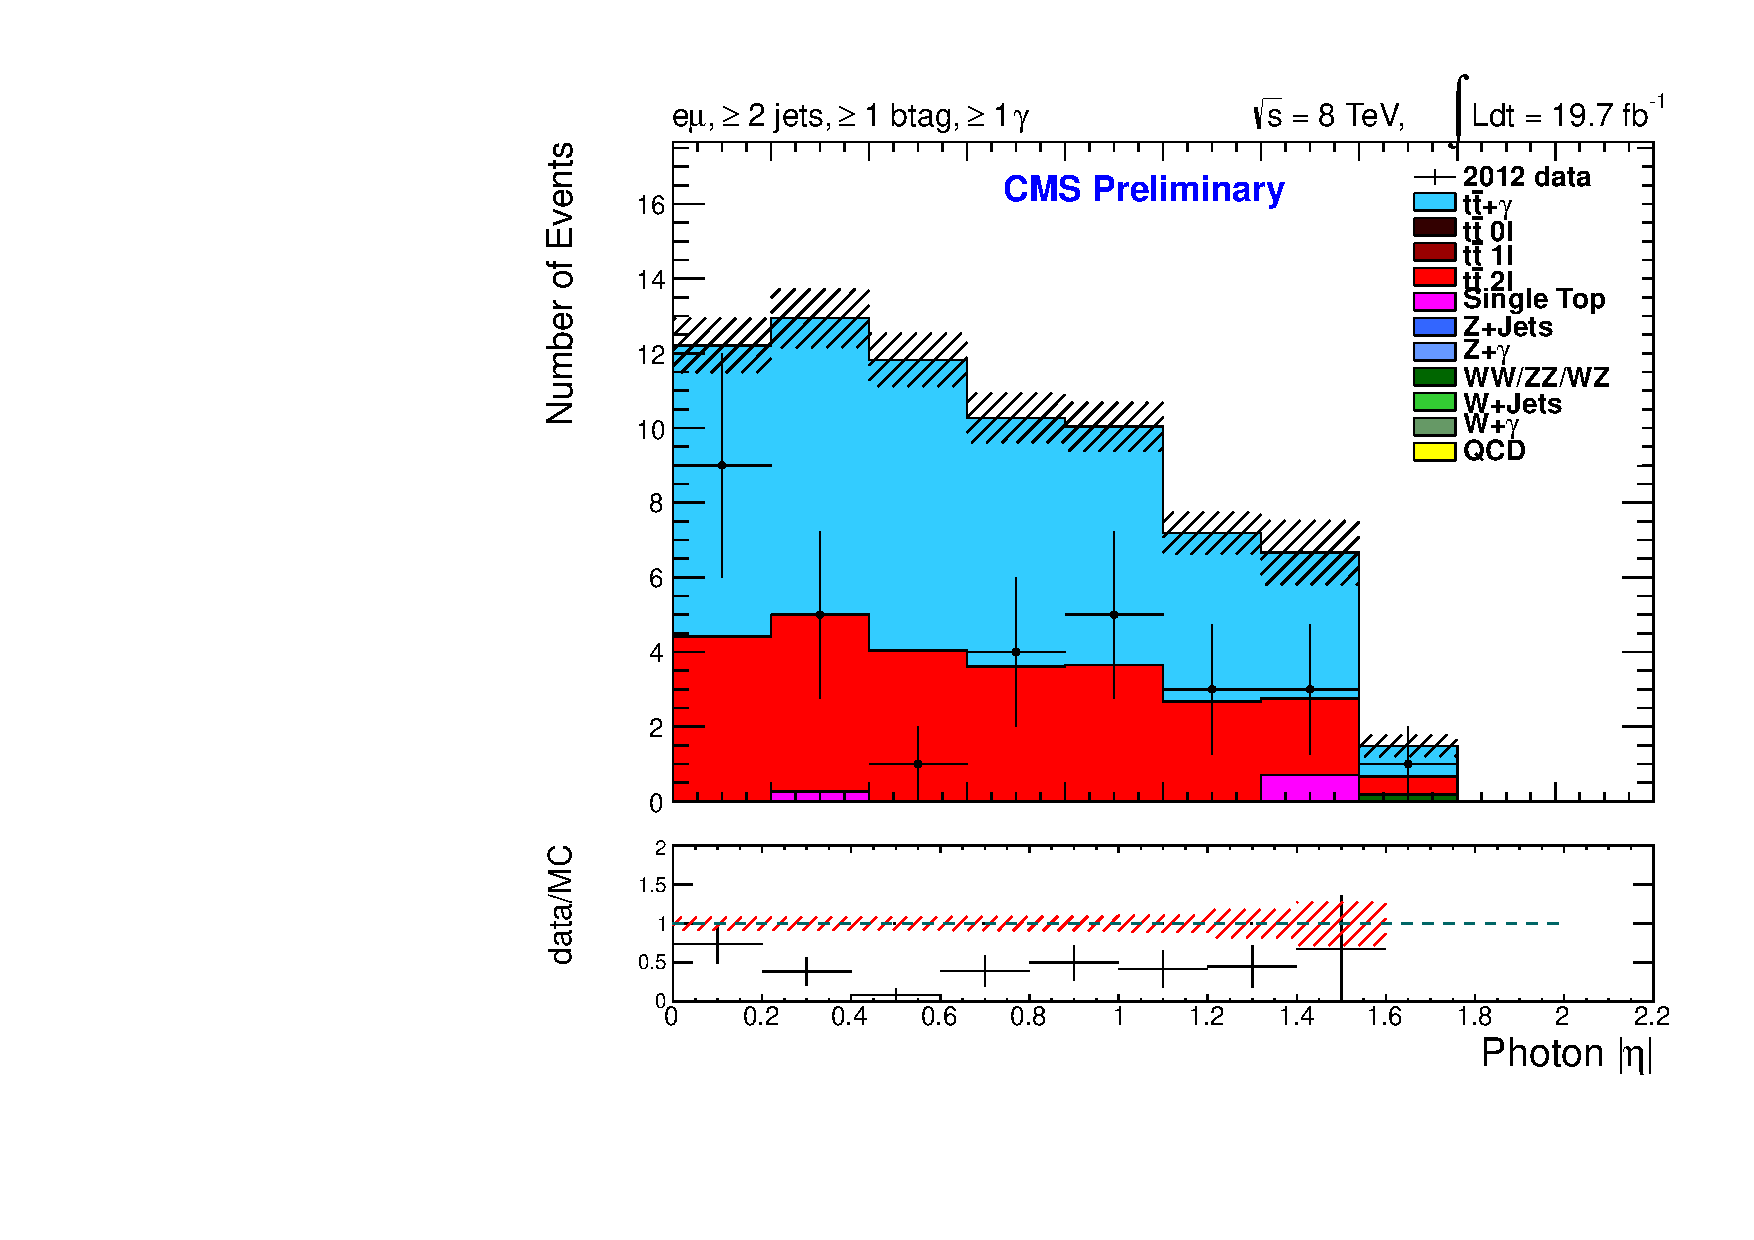
\includegraphics[width=0.5\textwidth]{Plots/ControlPlots/TTbarPhotonAnalysis/EMu/Photons/SignalPhotons/Photon_AbsEta_splitTTbar_ratio.pdf} 
% \end{center}
\caption{Comparison of photon E$_{T}$ and $|\eta|$ distributions in data and simulation in the $\mu^{+}\mu^{-}$, $e^{+}e^{-}$, and $e\mu$ channels after photon selection.}
\label{fig-photonSelectionETandEta}
\end{figure}

\subsection{Cut based photon identification}

The cut-based photon isolation requirements are taken from the recommended values \cite{CutBasedIsolation2012}, with the inclusion of supercluster footprint-removed isolation (see Section \ref{subsec-SCFR}). They are described below.

\begin{description}

\item[Electron Conversion Veto] A boolean to help distinguish an electron from a photon. A track seed should not be seen in the pixel detector when identifying a photon. 

\item[Tower Based H/E] The ratio of energy deposited in the HCAL divided by the fraction of energy deposited in the ECAL. The ratio is required to be less than 5\%.

\item[Shower Width $\sigma_{i\eta i\eta}$] The shower shape weighted by energy, is defined as: 

\begin{equation}
\sigma_{i\eta i\eta} = \left(\frac{\sum(\eta_i - \bar{\eta})\omega_i}{\sum\omega_i}\right)^{1/2}; \quad \bar{\eta} = \frac{\sum\eta_i\omega}{\sum\omega_i}; \quad  \omega_i = \text{max}\left(0, 4.7 +
\text{log}\frac{E_i}{E_{5\times5}}\right).
\end{equation}

This is a key variable in this analysis and will be discussed in greater detail in Section \ref{subsec-BackgroundEstimation}.

\item[Charged Hadron Isolation] The isolation of charged hadrons with energy density correction, $\rho$, applied. The requirement is given as $I_{Char.had} < 1.5 + 0.04 \times E_T(\gamma)$ GeV. 

\item[Neutral Hadron Isolation] The isolation of neutral hadrons with energy density correction , $\rho$, applied. The requirement is given as $I_{Neut.had} < 1.0 + 0.005 \times E_T(\gamma)$ GeV. 

\item[Photon Isolation] The isolation of the photon, $I_{\gamma}$, with energy density correction applied. The requirement is given as $I_{\gamma} < 1.0 + 0.005 \times E_T(\gamma)$ GeV.


\item[Supercluster footprint-removed Charged Hadron Isolation] The supercluster footprint-removed isolation of charged hadrons with energy density correction, $\rho$, applied.
Cut given as $I_{char.had} < 5 \ \text{GeV} $. 

\item[Supercluster footprint-removed Neutral Hadron Isolation] The supercluster footprint-removed isolation of neutral hadrons with energy density correction , $\rho$, applied.
Cut given as $I_{neut.had} < 1.0 + 0.005 \times E_T(\gamma)$ GeV. 

\item[Supercluster footprint-removed Photon Isolation] The supercluster footprint-removed isolation of the photon $I_{\gamma}$, with energy density correction applied. Cut given
as $I_{\gamma} < 1.0 + 0.005 \times E_T(\gamma)$ GeV. 

\end{description}

It must be noted that only supercluster footprint-removed charged hadron isolation is used in this analysis, whereas PF isolation is used for neutral hadron and photon isolation as described above. This is because it is used in the modelling of background events.

\subsection{Final state radiation suppression}

It is crucial that initial and final state radiation (ISR/FSR) is modelled correctly for this analysis as photons from initial and final state radiation are not considered as signal and therefore  $\Delta R$  constraints are applied to remove these events. The definition of isolation has been modified from the recommended values in order to make the data-driven estimate of the selection purity more robust. The requirements are as follows:

\begin{description}
\item[$\Delta R(\gamma, leptons)$] In order to reduce FSR in final state leptons, e.g photons radiated off high $p_T$ muons, a minimum distance criterion in the $\eta - \phi$ plane is implemented. The requirement is given as $\Delta R(\gamma, leptons) > 0.3$.

\item[$\Delta R(\gamma, jets)$] In order to reduce FSR from final state partons. A requirement of $\Delta R(\gamma, jets) > 0.3$ is applied, where $\Delta R(\gamma, jets)$ is the angular separation between the photon and the nearest jet.

\item[$\Delta R(leptons, jets)$] In order to reduce FSR from final state partons. A requirement of $\Delta R(leptons, jets) > 0.3$ is applied, where $\Delta R(leptons, jets)$ is the angular separation between the leptons and the nearest jet.
\end{description}

A significance test was performed in an attempt to optimise the $\Delta R$ cut between final state leptons and jets, however this proved inconclusive due to an initial cut of $\Delta R > 0.1$ at generator level. Figure \ref{fig-photonDRjets} shows the $\Delta R$ distributions after photon selection.

\begin{figure}
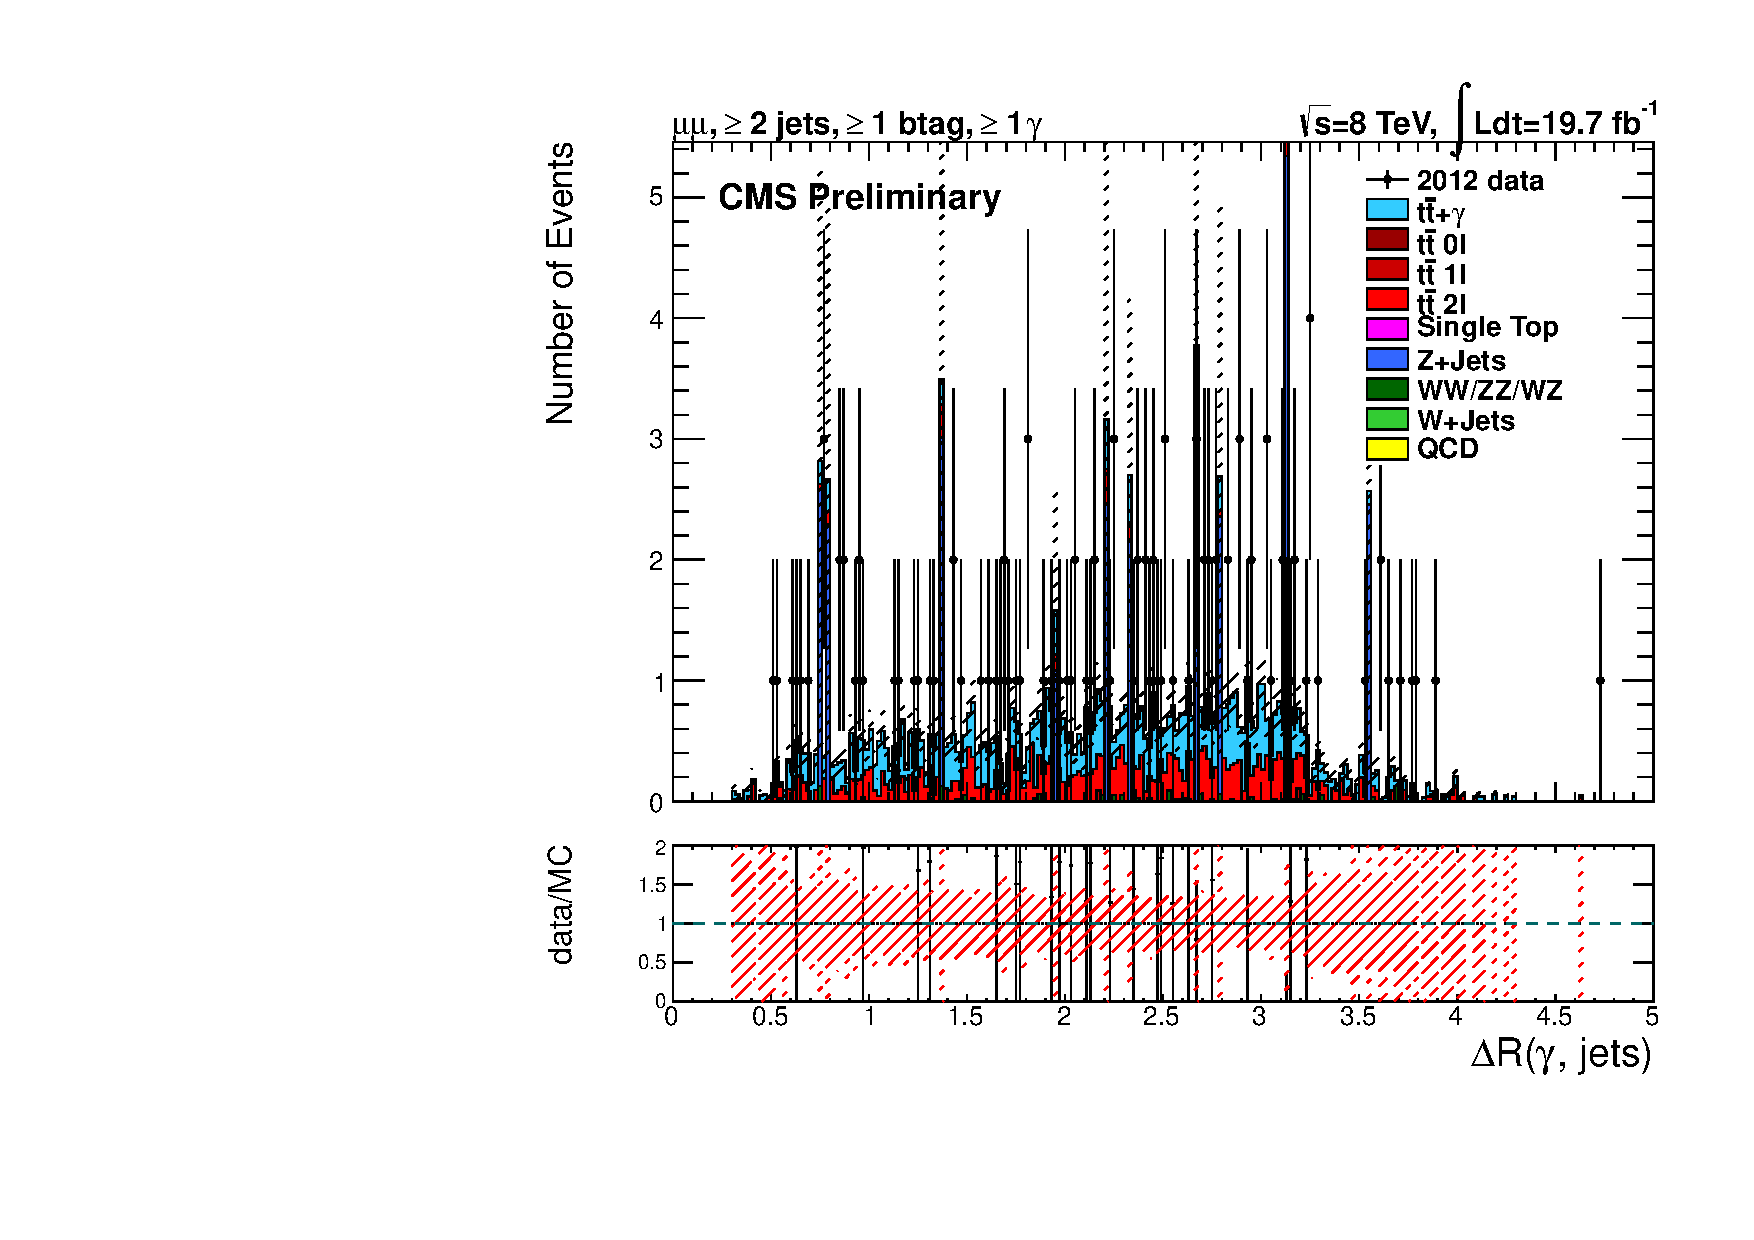
\includegraphics[width=0.5\textwidth]{Plots/ControlPlots/TTbarPhotonAnalysis/MuMu/Photons/SignalPhotons/Photon_deltaR_jets_splitTTbar_ratio.pdf}
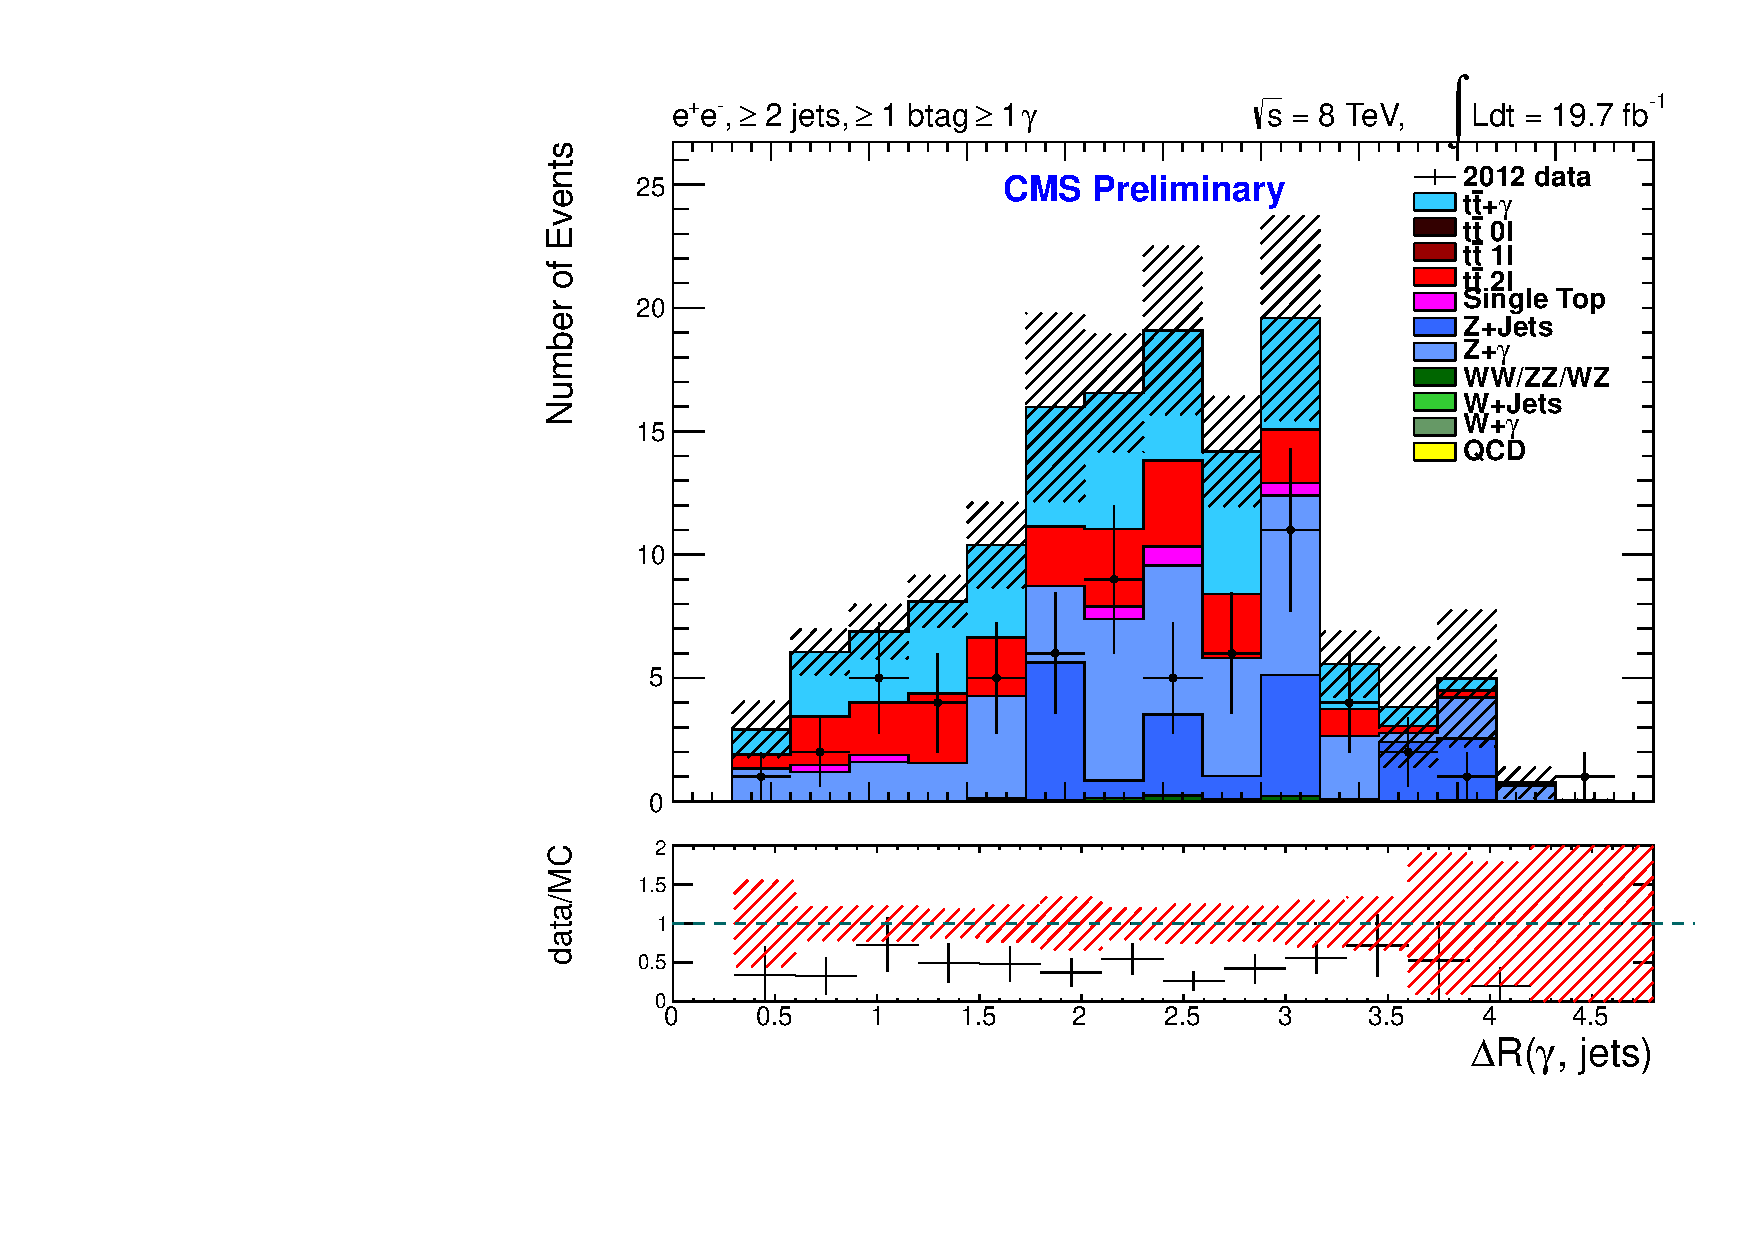
\includegraphics[width=0.5\textwidth]{Plots/ControlPlots/TTbarPhotonAnalysis/EE/Photons/SignalPhotons/Photon_deltaR_jets_splitTTbar_ratio.pdf}\\
\begin{center}
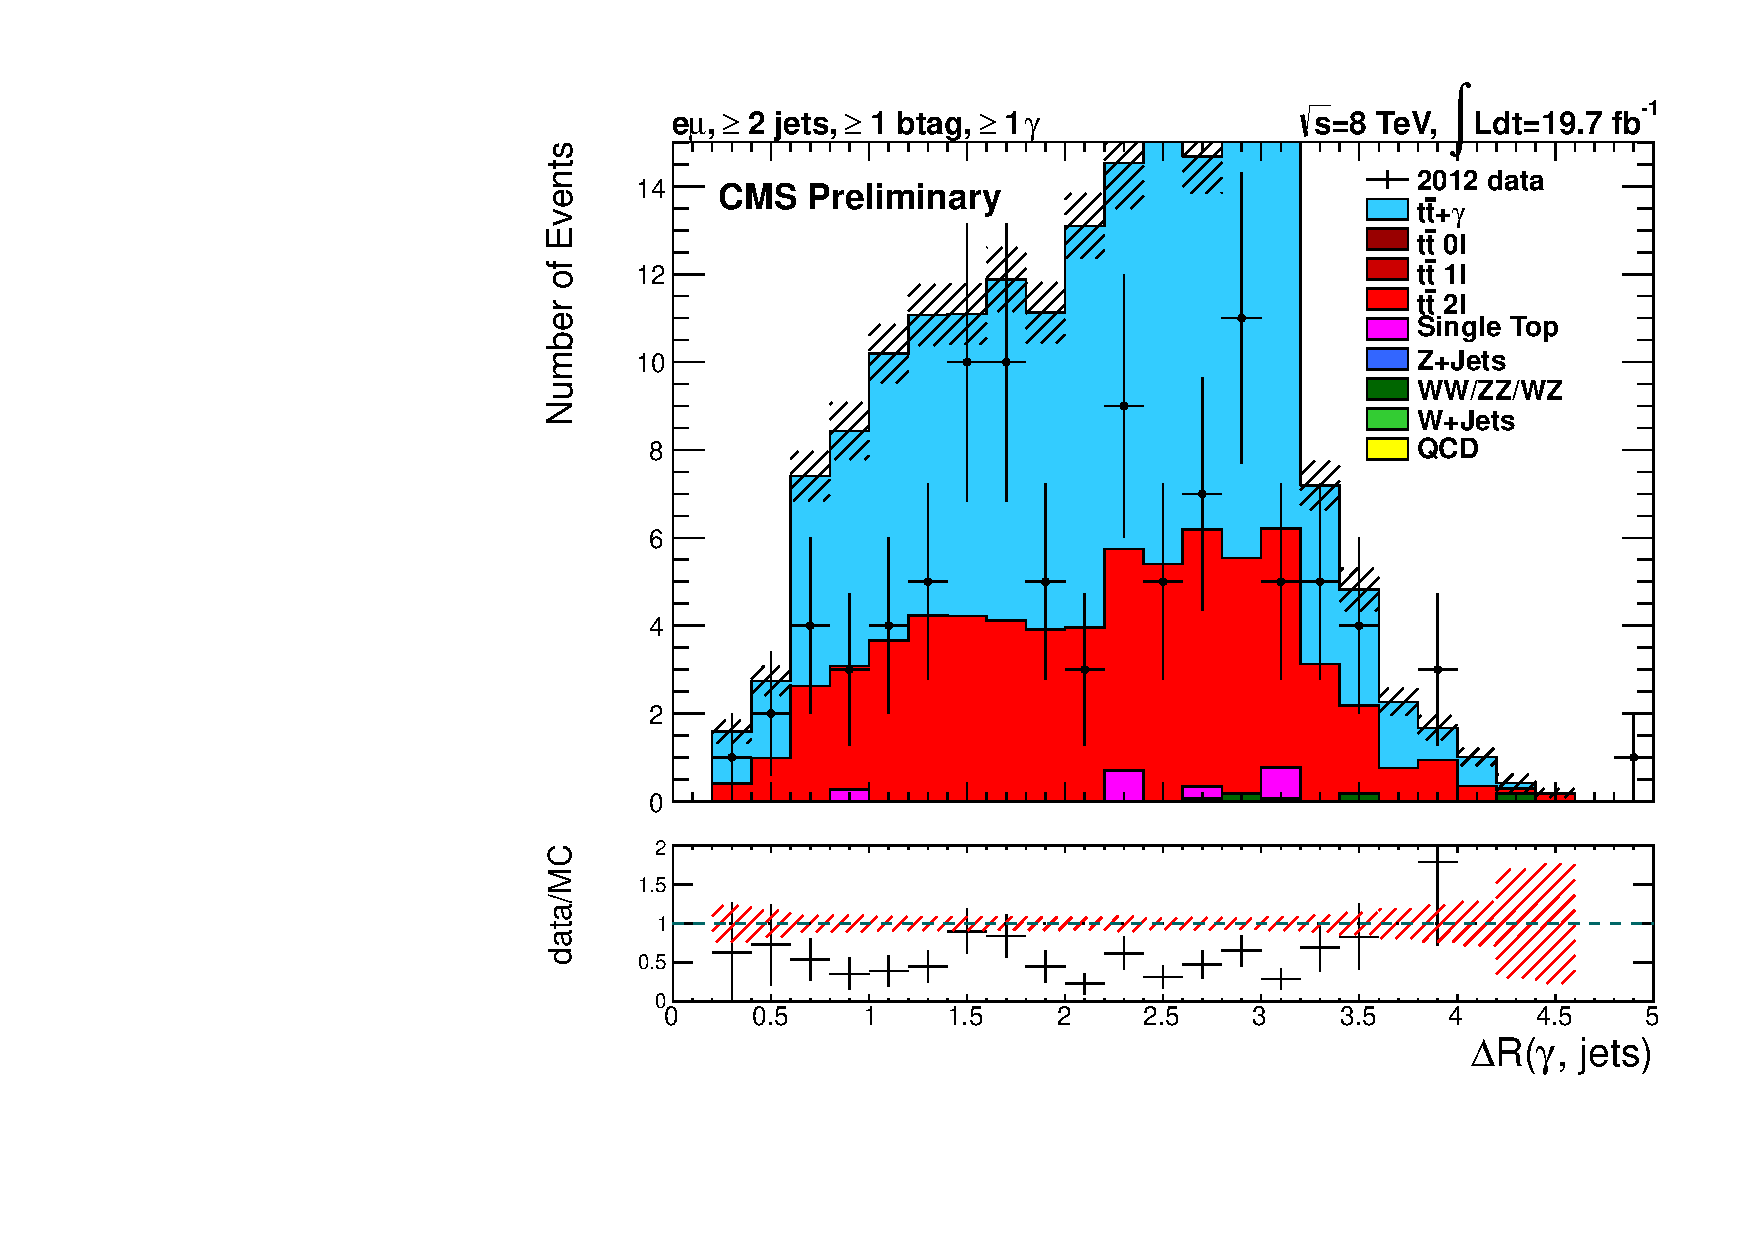
\includegraphics[width=0.5\textwidth]{Plots/ControlPlots/TTbarPhotonAnalysis/EMu/Photons/SignalPhotons/Photon_deltaR_jets_splitTTbar_ratio.pdf}
\end{center}
\caption{Comparison of the $\Delta R(\gamma, jets)$ distributions in data and simulation in the $\mu^{+}\mu^{-}$, $e^{+}e^{-}$, and $e\mu$ channels after photon selection.}
\label{fig-photonDRjets}
\end{figure}

The distributions for the other photon variables can be seen in Figure \ref{subsec-photonVariables}


\subsection{Supercluster footprint-removal for photon isolation} \label{subsec-SCFR}

The $t\bar{t}+\gamma$ analysis uses a method of removing the photon energy deposit, or ``footprint", from the isolation cone in order to remove the energy deposits of the selected photon from the isolation sum, and thus minimise correlation the between shower shape and isolation components in our signal process --- supercluster footprint removal (SCFR). With this method the footprint is, effectively, cleaned so that the isolation sum is not biased from the presence of the photon at the centre of the cone. Shower-shape variables, defined within the supercluster, are then decoupled from the isolation computation, defined outside of the supercluster. When the footprint of the photon has finally been removed, the isolation sum for prompt photons is due only to pileup and underlying events. The process calculates each isolation component individually, however only the charged hadron component of the isolation sum is considered using this technique, which is then used to model our background and signal processes. This method was first used in the measurement of the diphoton cross-section with 7 TeV data \cite{diffxsectdiphoton}. Usage of this results in an improvement in the agreement between data and MC for ECAL detector-based isolation, better discriminating power against the misidentification of photons, and it allows the use of a fully data-driven method for constructing the template fit.

The photon isolation is defined as the sum of the transverse momenta of all particles falling within the isolation cone surrounding the photon candidate. The isolation cone is defined to be within a $\Delta R < 0.3$, where $\Delta R = \sqrt{(\Delta\eta)^2+(\Delta\phi)^2}$. The momentum of the prompt photon should not contribute to the isolation sum, and thus particles found close to the photon footprint are not included within the sum. 

SCFR is a purely geometrical procedure that is computed as follows:

\begin{description}
	\item[Step 1]: Propagate the PF candidate trajectory from the primary vertex to the surface of the ECAL, taking into account the magnetic field when considering charged hadron candidates. The impact parameter, $d_z$, is calculated in the z-axis direction with respect to the primary vertex, neglecting the transverse distance, $d_{xy}$. 
	\item[Step 2]: If the propagated PF candidate is found to hit the surface of a crystal lying within the supercluster, then the candidate is removed from the isolation sum, as shown in Figure \ref{fig-SCFR}. The PF candidate is allowed to fall within a volume of 25\% of the crystal size around the crystal, in order to account for the fact that the PF candidate's energy deposit has a finite extension in the ECAL, and thus has a reasonably large effect at the edges of the supercluster. 
\end{description}

This ensures that such that the supercluster shape defines the region that is excluded from the isolation cone in each event.

In the standard particle flow algorithm isolation is calculated on an individual basis for PF candidates can be divided into three groups: Charged hadrons, neutral hadrons, and photons. This procedure carries potential pit-falls, as described below:

\begin{itemize}
	\item When computing the isolation sum, any energy deposit that is not associated with a reconstructed particle is not included within the sum.  
	\item When reconstructing a photon, its energy may be dispersed over a large radius within the detector, and thus reconstructed as several particles. This will greatly affect the isolation of the photon.
\end{itemize}

This does not have too much of an impact when using the standard cut-based particle identification methods, such as those used in this analysis. However, as we are interested in the isolation profile shape, some improvements must be made. 

Supercluster footprint-removed isolation is applied to PF candidates, whereas PF isolation is applied to identified particles. This reduces the probability for the first of these issues to occur. The second pit-fall is a result of the leakage of energy from the photon into the isolation cone around the supercluster. Therefore, a different method for defining the isolation cone must be implemented to overcome this problem.  Summing the transverse momentum of particle flow candidates that fall within the isolation cone, but which are not close to the supercluster in the ECAL. The $\eta$ and $\phi$ coordinates of the supercluster are calculated by checking the position of hits recorded in the tracker, and if a PF candidate that has been propagated to the surface of the calorimeter lies within the supercluster, enlarged by 25\%, then the photon is not considered isolation and thus the candidate is not added to the isolation sum. The standard CMS implementation for energy density correction, $\rho$, is applied to the isolation to account for pileup. 

\begin{figure} 
\begin{center}
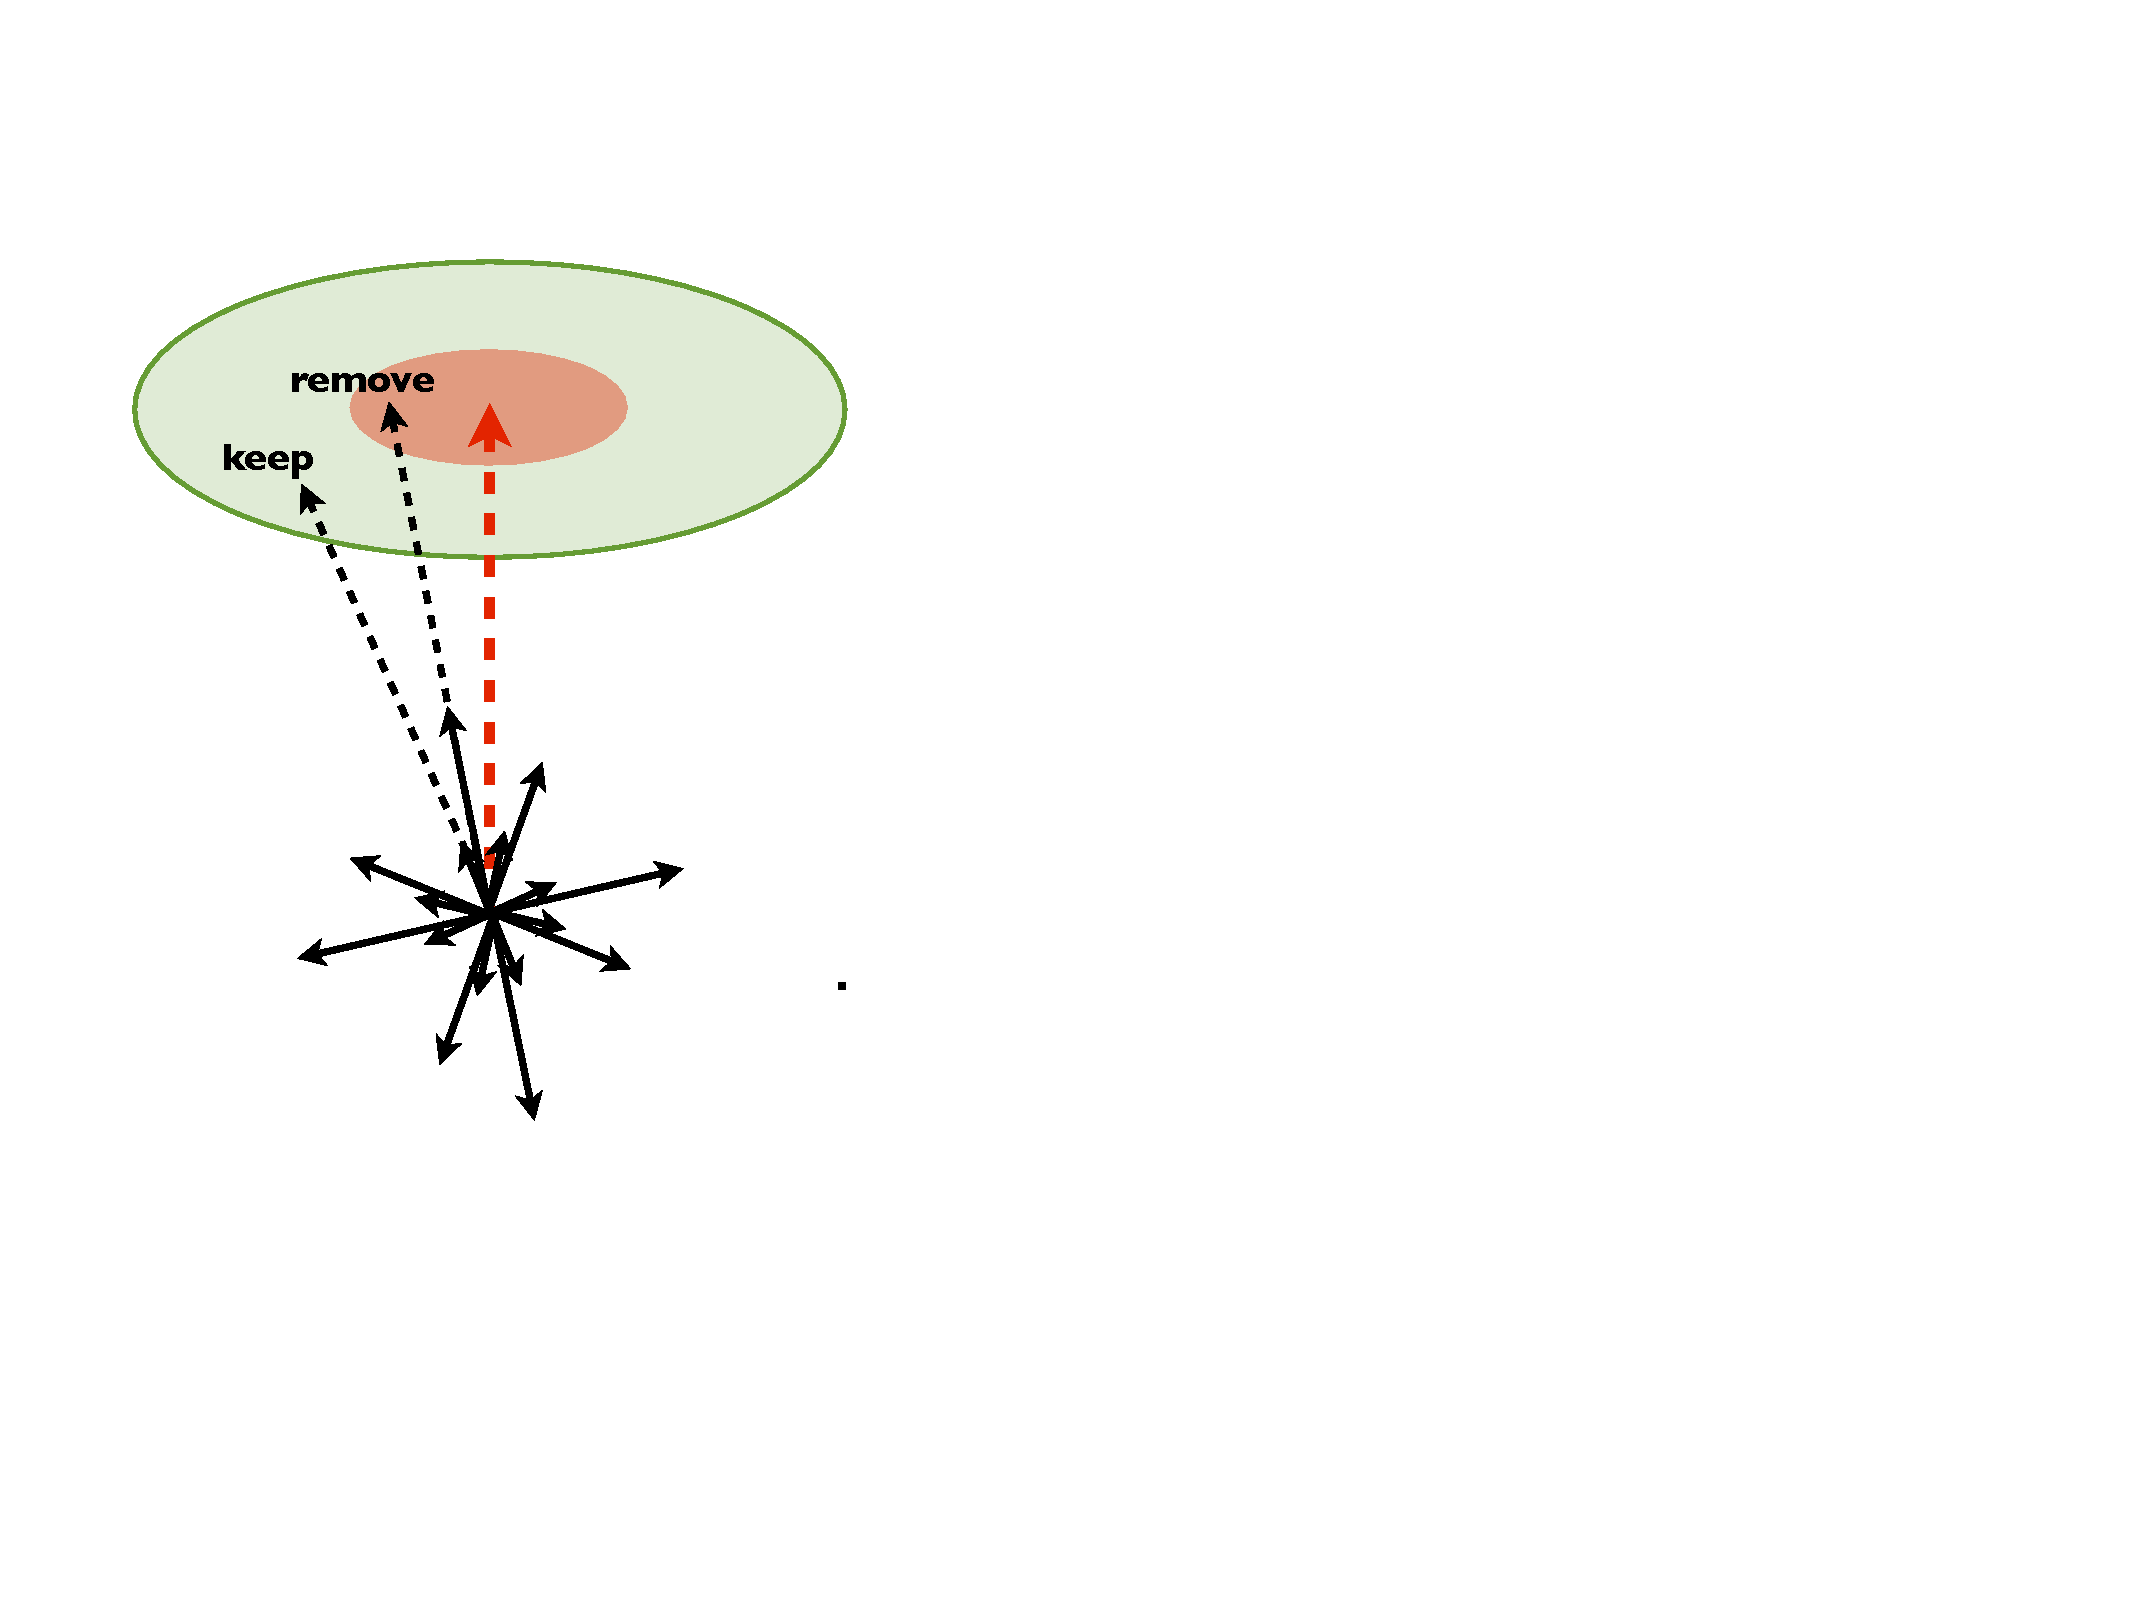
\includegraphics[width=0.4\textwidth]{Figures/RandomCone3.pdf}
\end{center}
\caption{Graphical representation of the PF candidate footprint (red) from the primary interaction vertex, within the isolation cone (green). \cite{MarcoThesis}}
\label{fig-SCFR}
\end{figure}

\section{Phase Space Overlap Removal} \label{sec-PhaseSpaceOverlapRemoval}

Events of the $t\bar{t}+\gamma$ process lie within a small region of $t\bar{t}$ phase space (see Figure \ref{fig-photonphasespace}), and thus our signal sample events are expected to overlap with TTJets events in the case where a hard photon is radiated by initial state quarks, top quarks, b quarks, W and its decay products: electrons, muons, and their corresponding neutrino. In order to prevent the double counting of events we apply an overlap removal procedure to remove such events from our TTJets samples. In order for an event to be considered as overlapping with TTGamma, an event has to have at least one generator-level photon with the following properties:

\begin{itemize}
	\item p$_T(\gamma) > 13$ GeV
	\item $|\eta| < 3.0$
	\item Only gluons, bosons, or leptons are in the parents list. This ensures that photons from $\pi^0$ decays are not considered as signal
	\item $\Delta R(\gamma, other) > 0.2$ where other particles include leptons, b quarks and final state particles (hadrons, charged leptons, photons) with transverse momenta above $5 \GeV$.
\end{itemize}

The last cut is implemented in order to suppress photons from showers. In such cases the information from the parent particle will show that a photon is radiated by an electron, however the photon may be collinear with it. In particular, in TTJets dilepton events, such as described in this analysis, where a considerable fraction of the reconstructed photons comes from electrons radiating photons.

 Similarly, we also observe an overlap between $Z+Jets$ and $Z+\gamma$ processes, and between W+Jets and WGamma samples, for the same reasons as described above. The phase space overlap removal procedure is applied on Z+Jets and W+Jets samples to remove events containing generator-level photons. Events containing generated photons are removed in the case in which they are from initial state radiation (emitted from the colliding partons) or final state radiation (emitted from W or Z bosons or their decay products), since these are already included in the WGamma and ZGamma simulations. The overlap removal procedure removes approximately one percent of the events in the W+Jets sample, and approximately three to four percent of the events from the TTJets and Z+Jets samples.

\begin{figure} 
\begin{center}
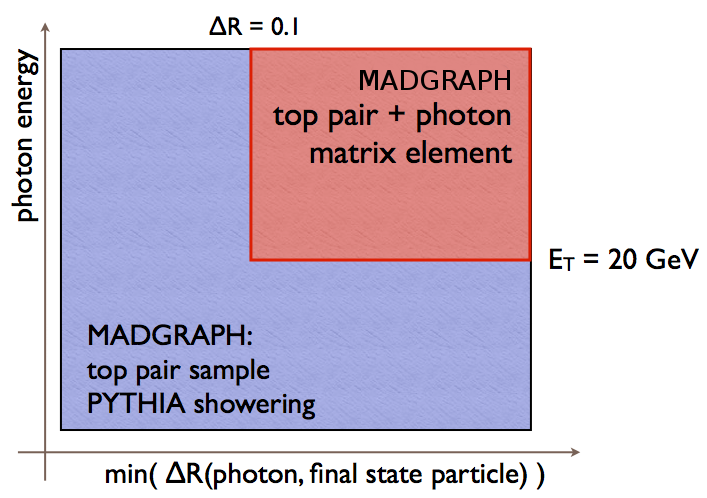
\includegraphics[scale=0.5]{Figures/photonphasespace2.png}
\end{center}
\caption{Graphic representation of the $t\bar{t}+\gamma$ phase space relative to the $t\bar{t}$ phase space.}
\label{fig-photonphasespace}
\end{figure}

\section{Corrections to simulated events} \label{sec-SimulatedEventsCorrection}

Although we heavily rely on simulation to model the processes that we are interested in, there are various processes that arise as a product of hadron-hadron collisions in which it does not always perfectly describe. In order to model a process accurately, we want to have a model that lies as close to the observed data as possible without introducing any form of bias. Therefore, we calculate a Scale Factor (SF) to account for the mismatch of data against simulation for each process. We must also calculate a weighting for individual MC samples in order to reweight the total number of generated events as follows:  

\begin{equation}
SF_{MC} = \frac{\lumi \times \sigma}{N_{events}}
\end{equation}

where $\lumi$ is the integrated luminosity of the data, $\sigma$ the theoretical cross-section of the simulated process, and $N_{events}$ the number of processed events for a particular process. The scale factors are calculated on an event-by-event basis and are defined as the product of individual scale factors for each correction type, as shown in Equation \ref{eqn-SFProduct}. 

\begin{equation}
SF = SF_{MC} \times SF_{Trig} \times SF_{Lep} \times SF_{PU} \times SF_{Btag}
\end{equation} \label{eqn-SFProduct}

A reweighting of the p$_T$ distribution of top pairs is also incorporated and described in Section \ref{}. The different event correction types are described below.

\begin{description}
	\item[Pileup Reweighting] The number of pileup interactions per event varies depending on many factors, such as the luminosity of collisions. Generated events are produced with a nominal number of pileup interactions and this must be corrected in order to match with that observed in data. To correct the number of pileup interactions per event, we must have knowledge of the number of pileup in simulation,the luminosity of the dataset we are correcting for, and the total inelastic cross-section of proton-proton collisions, such that $N_{PU} = \lumi \times \sigma_{pp}$.    
	\item[B-tagging Reweighting] It is observed that the efficiency of correctly tagging a b-jet varies in simulation compared to that observed in data. The efficiency is calculated as the number of b-tagged jets over the total number of jets, given as 
	\begin{equation}
	\epsilon_f = \frac{N_f^{b-tagged}}{N_{f}^{Total}}
	\end{equation}
	where f is the flavour of jet. We apply a p$_T$-dependent scale factor to simulated events to account for this discrepancy \cite{CMS-DP-2013-005} following the BTV group prescription. To calculate the weight for each event containing one of more b-tags, we find the probability of having exactly zero b-tags ($\Pi_i = \left(1 - SF_i\right)$), and iterating over the events found to contain one b-jet in simulation. We then calculate the probability of an additional b-jet to be $1 - \Pi_i\left(1 - SF_i\right)$.  
	\item[Lepton Efficiencies] Lepton efficiencies manifest in three forms: lepton trigger, isolation, and identification scale factors. Lepton triggers are used in simulation to replicate the triggers used in data, however this strategy does not always mirror the process accurately enough, and thus a trigger scale factor must be implemented to account for this difference. The trigger scale factor is computed using the tag-and-probe method \cite{tagandprobe} described in Section \ref{subsec-LeptonEfficiencies}. The efficiency is calculated as a function of p$_T$ and $\eta$, and is give by the ratio
	\begin{equation}
	SF_{Trig.} = \frac{\epsilon_{data}}{\epsilon_{MC}}
	\end{equation}
	The trigger scale factors used in this analysis were centrally produced by the CMS EGamma and Muon physics object groups for the 2012 data set and are defined as \ref{tab-leptonTriggerSFs}. The same technique can be applied when computing scale factors for lepton isolation and identification.  
	\item[Z+Jets Scale Factors]
\end{description} 

\section{Event selection cut flow} \label{sec-cutflow}

After all selection and identification requirements are applied, it is useful to see which selection requirements have the most impact. This is called the cut flow. Figure \ref{fig-CutFlow} shows the number of events after each step of the selection process for each decay channel, along with the ratio of number of events in data to that in the Monte Carlo. It is quite clear that QCD is the dominant process a priori any selection requirements. After the implementation of $t\bar{t}$ selection requirements the most dominant process becomes $t\bar{t}$, then becoming the signal $t\bar{t}+\gamma$ upon the inclusion of photon-specific selection requirements. 

An excellent agreement is observed between the data and simulation, disregarding the first bin of Figure \ref{fig-CutFlow}. This discrepancy between the data and MC can be attributed to the trigger not being applied to MC until the ``Cleaning \& HLT" step of the selection process, whereas it is initially applied to the data. A large reduction of QCD can be seen upon selecting two oppositely signed isolated leptons as multi-jet events seldom produce isolated leptons. The largest remaining backgrounds, other than $t\bar{t}$, are vector boson events ($W+jets$, $Z+jets$) and vector bosons with a radiated photon ($W+\gamma$, $Z+\gamma$). This is largely reduced in the $e\mu$ decay channel due to the selection of two oppositely-signed and opposite-flavour leptons. The events yields after each selection step, and for each Monte Carlo sample, is shown in Tables \ref{tab-cutflowMuMu}, \ref{tab-cutflowEE},and \ref{tab-cutflowEMu}, for each decay channel, respectively. 

\begin{figure} [h]
%\begin{center}
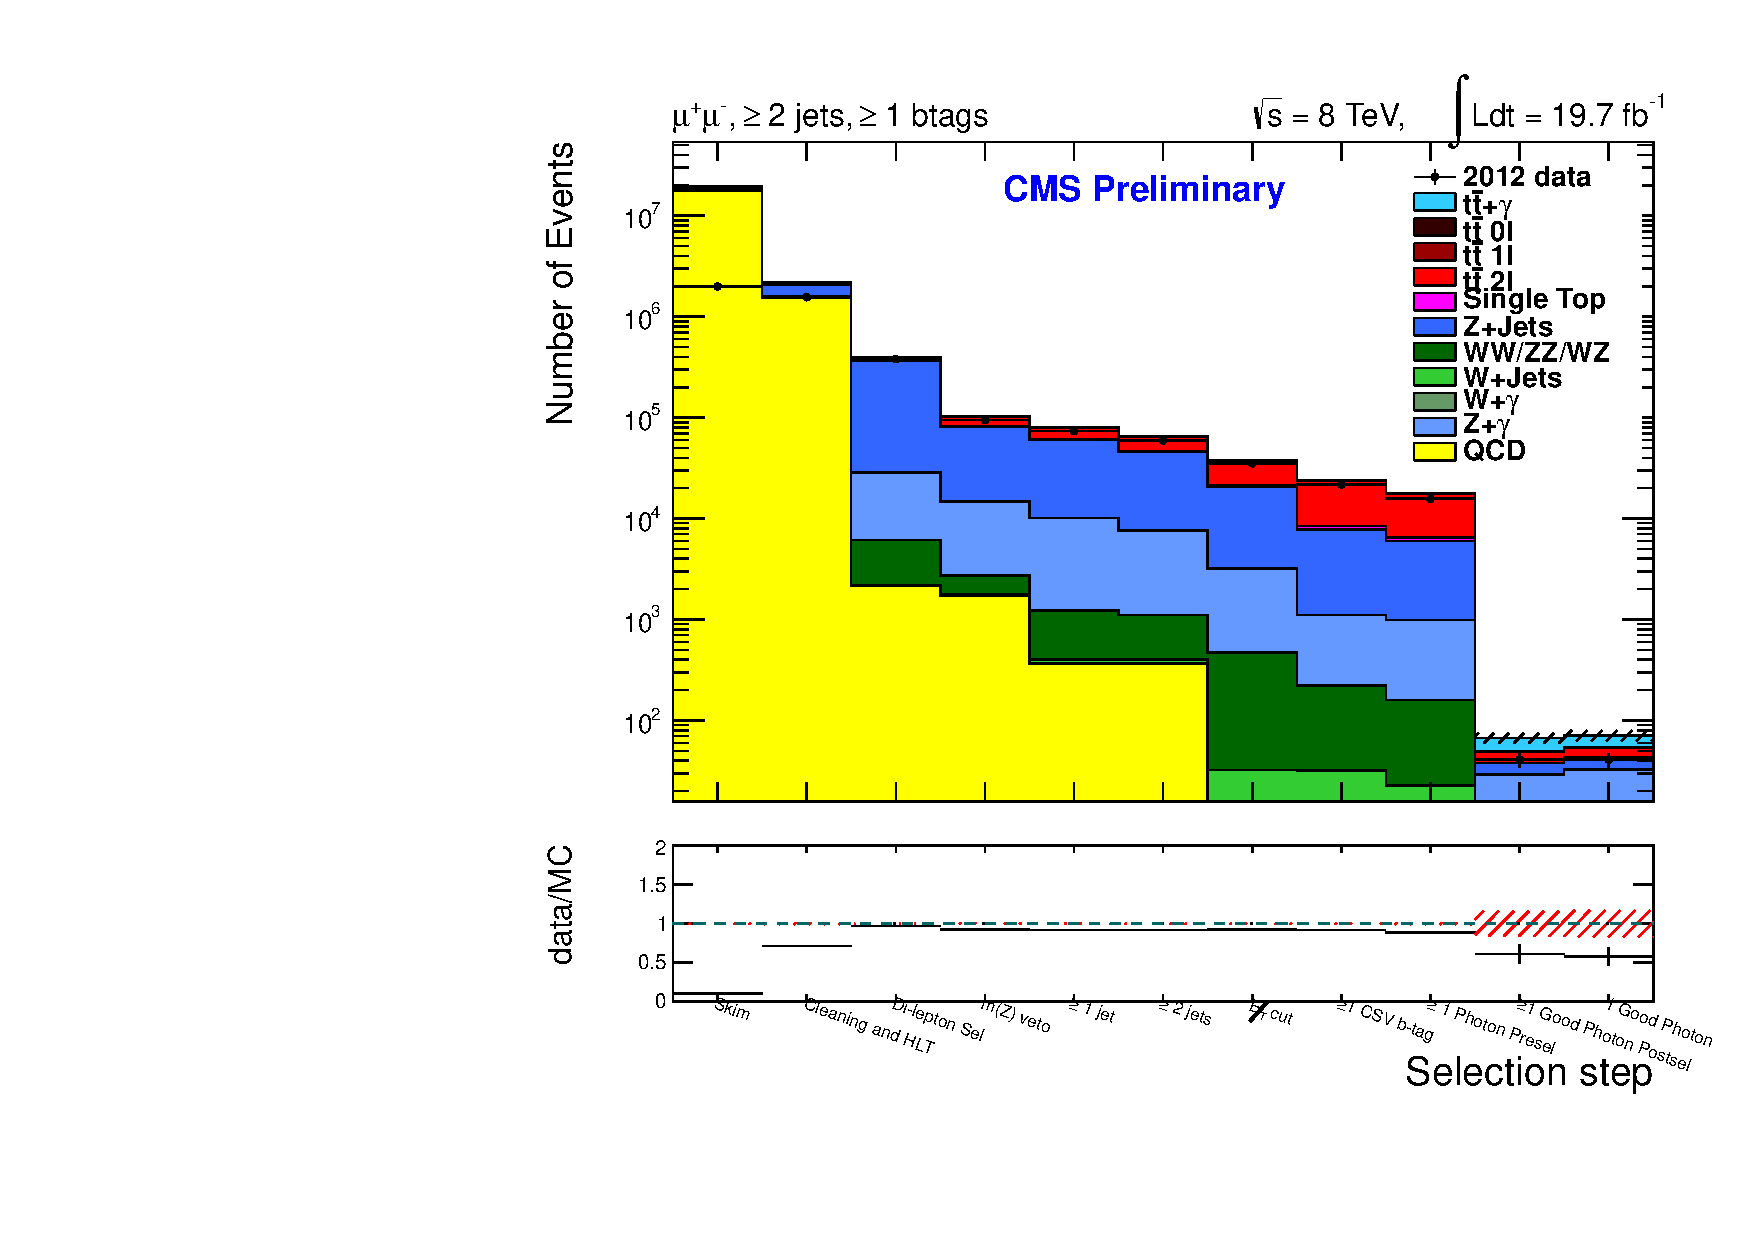
\includegraphics[width=0.5\textwidth]{Plots/ControlPlots/CutFlow/Log/TTbarMuMuRefSelection_splitTTbar_ratio.pdf}
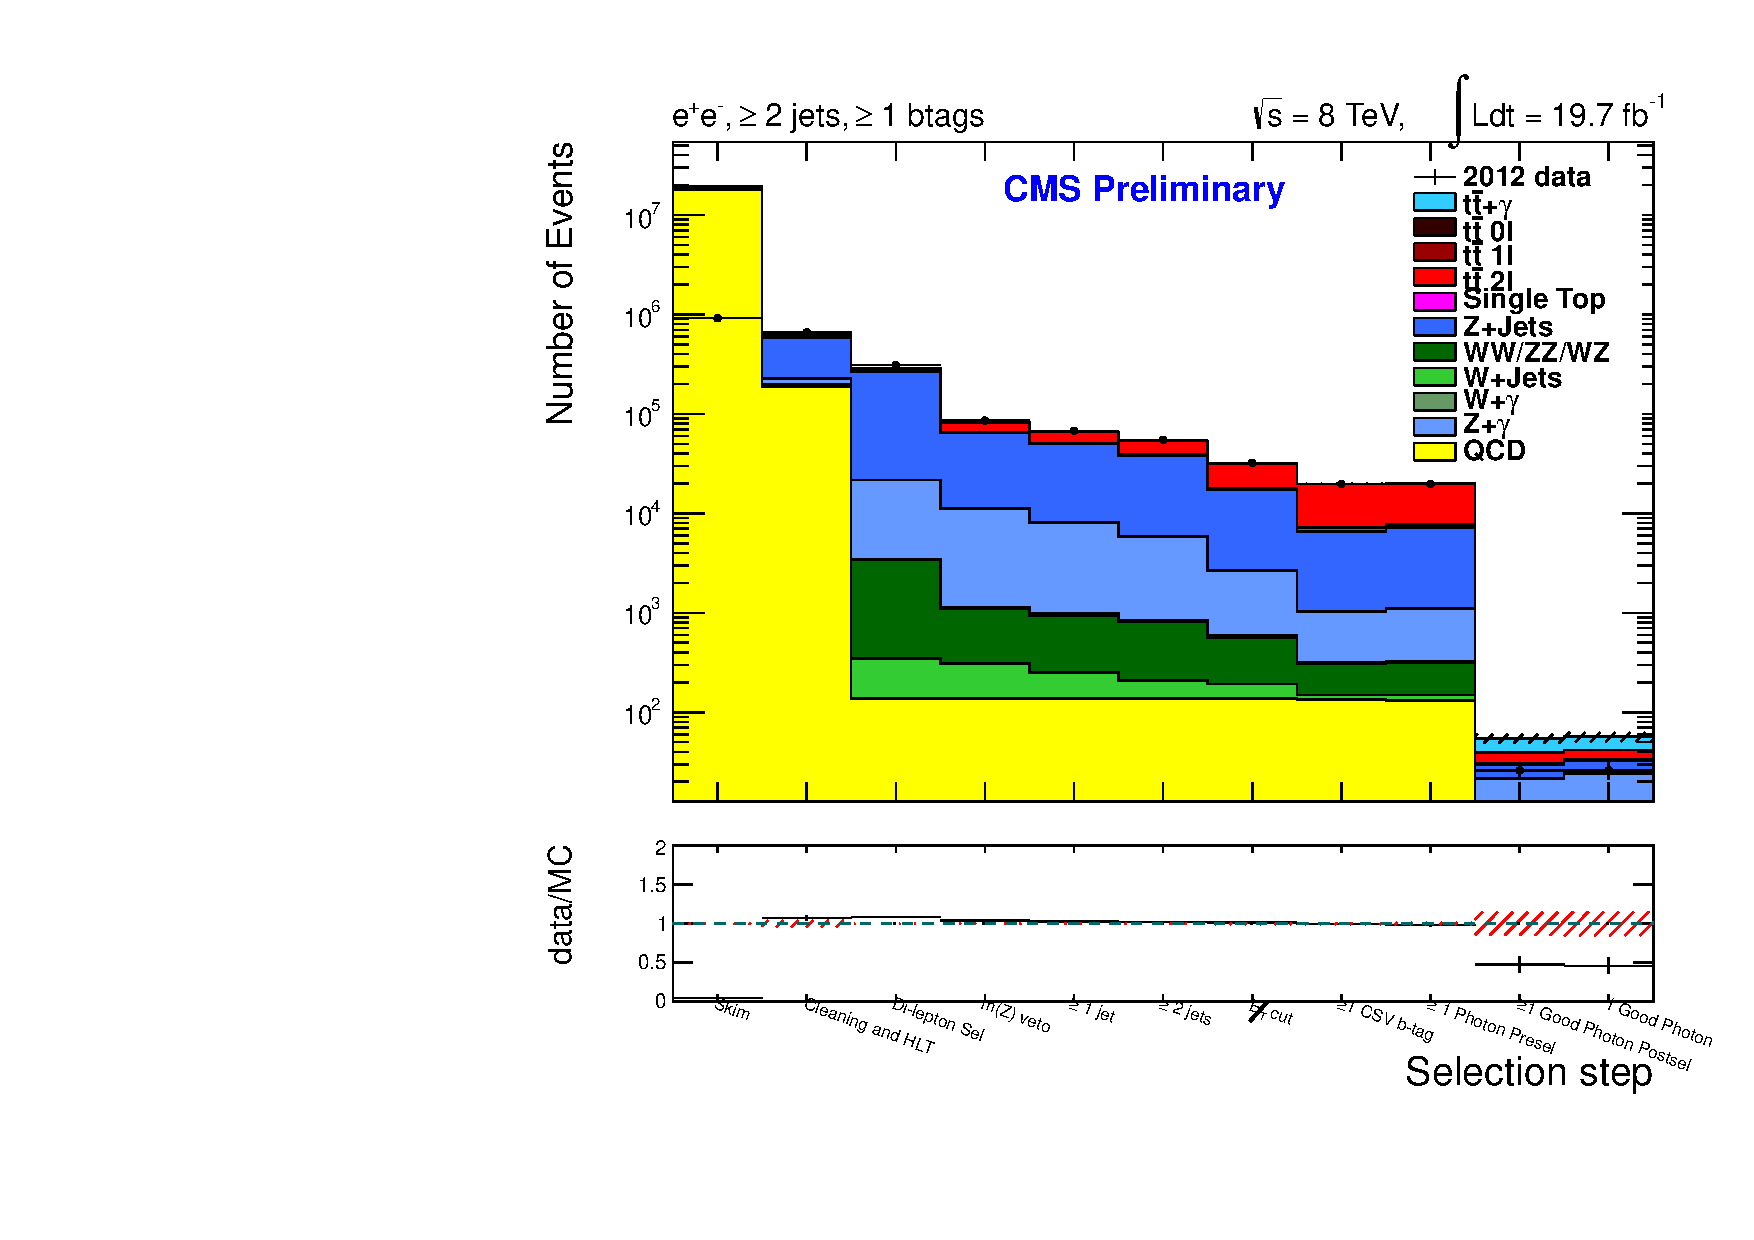
\includegraphics[width=0.5\textwidth]{Plots/ControlPlots/CutFlow/Log/TTbarEERefSelection_splitTTbar_ratio.pdf} \\
\begin{center}
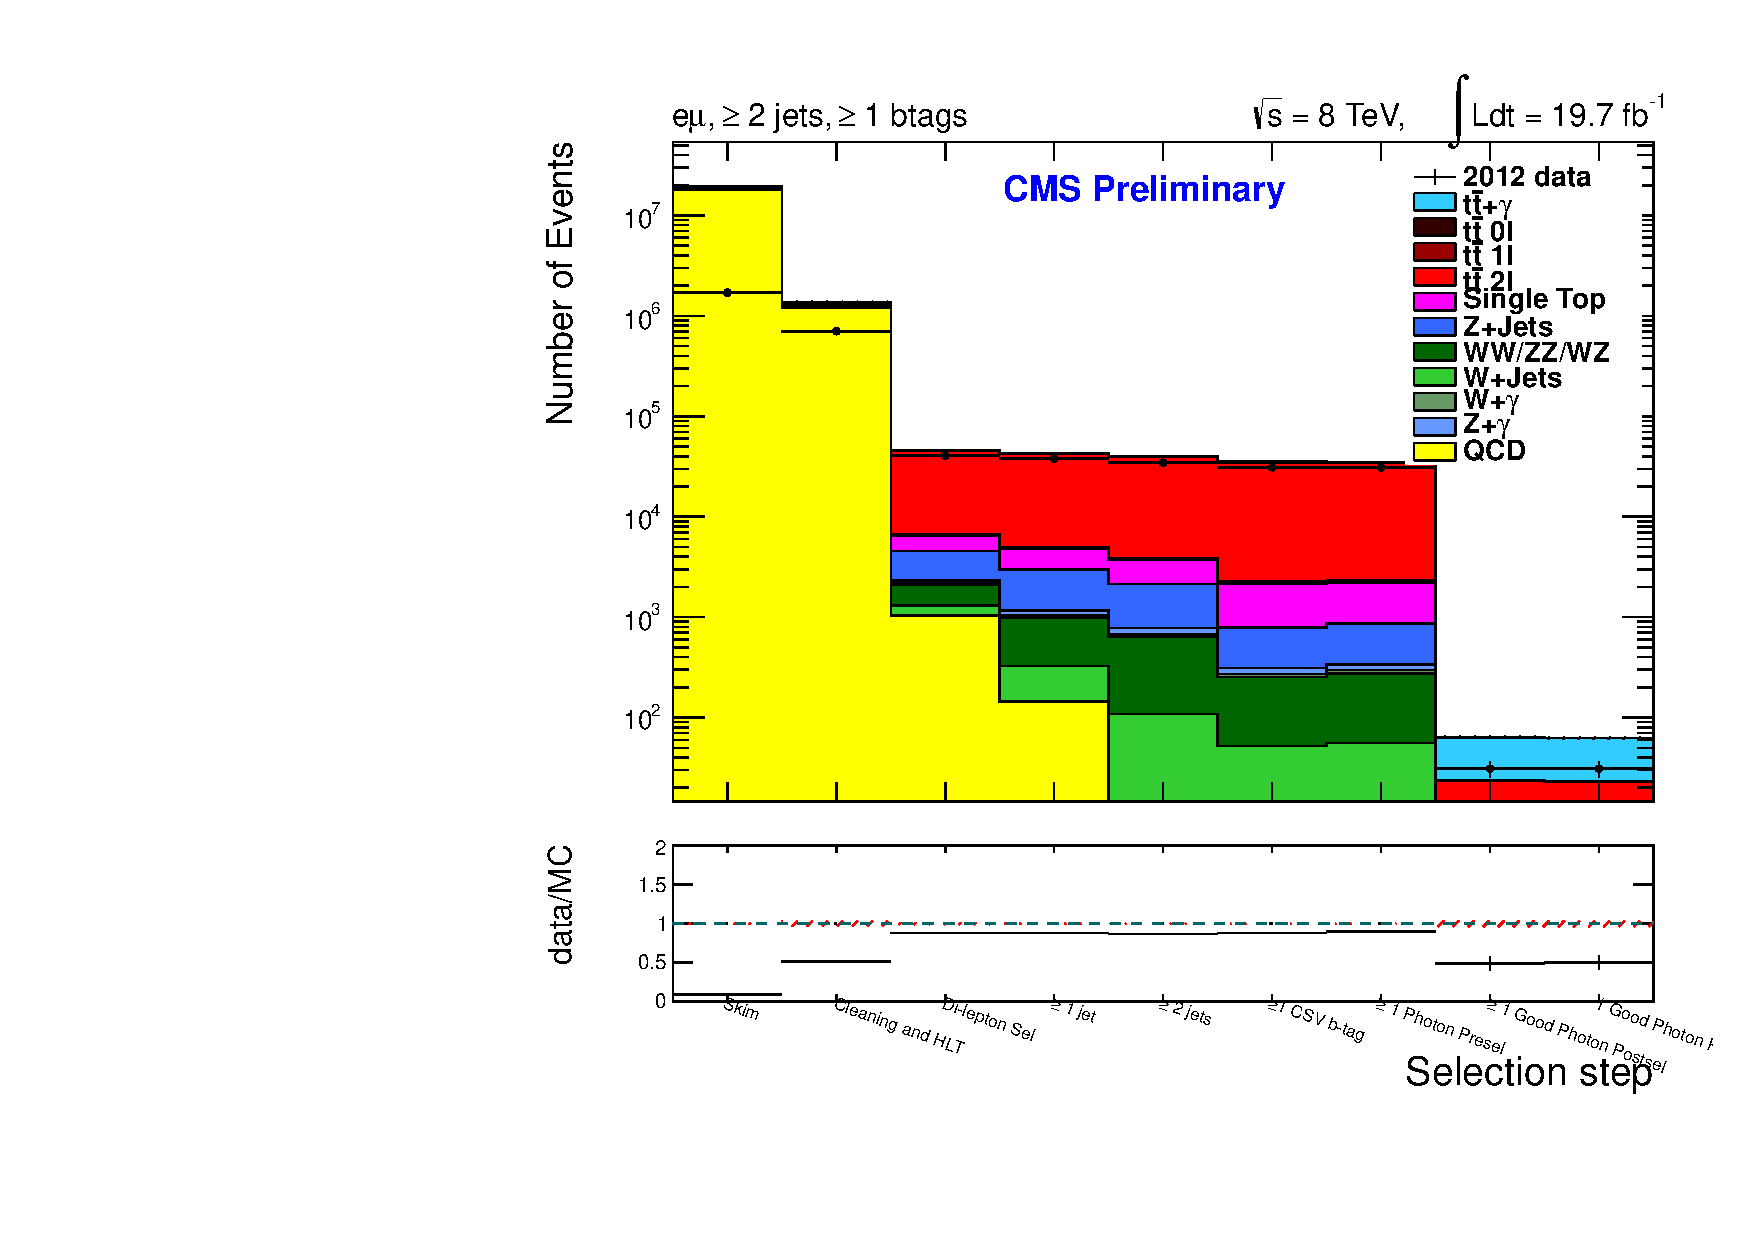
\includegraphics[width=0.5\textwidth]{Plots/ControlPlots/CutFlow/Log/TTbarEMuRefSelection_splitTTbar_ratio.pdf}
\end{center}
\caption{Cutflow plots showing the number of events remaining after individual cuts are introduced, comparing distributions in data and simulation in the $\mu^{+}\mu^{-}$, $e^{+}e^{-}$, and $e\mu$ channels.}
\label{fig-CutFlow}
\end{figure}

\begin{sidewaystable}[h!]
  \centering 
%  \caption{Cut Flow table for the $\mu^+\mu^-$ selection.}
%  \label{tab:mumu_cutflow}
\resizebox{\columnwidth}{!} {

\begin{tabular}{|l|l|l|l|l|l|l|l|l|l|l|l|l|l|}
\hline
\multicolumn{14}{|c|}{\textbf{Cut Flow table for the $\mu^+\mu^-$ selection}} \\
\hline
 & $t\bar{t}+\gamma$ & $t\bar{t} 0l$ & $t\bar{t} 1l$ & $t\bar{t} 2l$ & w+jets & z+jets & $W+\gamma$ & $Z+\gamma$ & diboson & single-t & qcd & all MC & data \\
 \hline
Skim & 3418 $\pm$ 12 \ & 16912 $\pm$ 37 \ & 132676 $\pm$ 113 \ & 137147 $\pm$ 81 \ & 166712 $\pm$ 1559 \ & 1013494 $\pm$ 1639 \ & 10326 $\pm$ 166 \ & 73574 $\pm$ 208 \ & 13909 $\pm$ 30 \ & 27811 $\pm$ 339 \ & 16621473 $\pm$ 136970\ & 18217451 $\pm$ 136990 \ & 1885535 $\pm$ 1373 \\
Cleaning and HLT & 952 $\pm$ 6 \ & 2925 $\pm$ 15 \ & 33828 $\pm$ 57 \ & 43049 $\pm$ 45 \ & 7927 $\pm$ 339 \ & 479975 $\pm$ 1117 \ & 321 $\pm$ 30 \ & 34586 $\pm$ 142 \ & 4920 $\pm$ 15 \ & 6677 $\pm$ 162 \ & 1389098 $\pm$ 19616\ & 2004257 $\pm$ 19652 \ & 1473970 $\pm$ 1214 \\
Di-lepton Sel & 274 $\pm$ 3 \ & 0 $\pm$ 0 \ & 139 $\pm$ 4 \ & 20006 $\pm$ 30 \ & 32 $\pm$ 20 \ & 324348 $\pm$ 901 \ & 2 $\pm$ 2 \ & 21270 $\pm$ 110 \ & 3579 $\pm$ 13 \ & 992 $\pm$ 22 \ & 1976 $\pm$ 556\ & 372618 $\pm$ 1065 \ & 359665 $\pm$ 600 \\
m(Z) veto & 245 $\pm$ 3 \ & 0 $\pm$ 0 \ & 117 $\pm$ 3 \ & 17856 $\pm$ 29 \ & 32 $\pm$ 20 \ & 63584 $\pm$ 430 \ & 2 $\pm$ 2 \ & 11378 $\pm$ 81 \ & 866 $\pm$ 8 \ & 886 $\pm$ 21 \ & 1601 $\pm$ 509\ & 96567 $\pm$ 672 \ & 89425 $\pm$ 299 \\
$\geq$ 1 jet & 225 $\pm$ 3 \ & 0 $\pm$ 0 \ & 97 $\pm$ 3 \ & 17305 $\pm$ 28 \ & 32 $\pm$ 20 \ & 47361 $\pm$ 381 \ & 2 $\pm$ 2 \ & 8374 $\pm$ 70 \ & 755 $\pm$ 7 \ & 838 $\pm$ 20 \ & 368 $\pm$ 261\ & 75357 $\pm$ 469 \ & 69447 $\pm$ 264 \\
$\geq$ 2 jets & 197 $\pm$ 3 \ & 0 $\pm$ 0 \ & 60 $\pm$ 2 \ & 16382 $\pm$ 27 \ & 32 $\pm$ 20 \ & 36544 $\pm$ 334 \ & 0 $\pm$ 0 \ & 6138 $\pm$ 60 \ & 636 $\pm$ 6 \ & 733 $\pm$ 19 \ & 368 $\pm$ 261\ & 61089 $\pm$ 430 \ & 56136 $\pm$ 237 \\
$\slash{E_{T}}$ cut & 183 $\pm$ 3 \ & 0 $\pm$ 0 \ & 55 $\pm$ 2 \ & 15343 $\pm$ 26 \ & 32 $\pm$ 20 \ & 16589 $\pm$ 224 \ & 0 $\pm$ 0 \ & 2553 $\pm$ 38 \ & 399 $\pm$ 5 \ & 689 $\pm$ 18 \ & 0 $\pm$ 0\ & 35843 $\pm$ 231 \ & 33323 $\pm$ 183 \\
$\geq$ 1 CSV b-tag & 167 $\pm$ 3 \ & 0 $\pm$ 0 \ & 44 $\pm$ 2 \ & 14090 $\pm$ 25 \ & 32 $\pm$ 20 \ & 6342 $\pm$ 145 \ & 0 $\pm$ 0 \ & 829 $\pm$ 23 \ & 169 $\pm$ 4 \ & 606 $\pm$ 17 \ & 0 $\pm$ 0\ & 22280 $\pm$ 151 \ & 20680 $\pm$ 144 \\\
$\geq$ 1 Photon Presel & 162 $\pm$ 2 \ & 0 $\pm$ 0 \ & 35 $\pm$ 2 \ & 10336 $\pm$ 21 \ & 23 $\pm$ 17 \ & 4749 $\pm$ 131 \ & 0 $\pm$ 0 \ & 774 $\pm$ 23 \ & 123 $\pm$ 3 \ & 419 $\pm$ 14 \ & 0 $\pm$ 0\ & 16620 $\pm$ 137 \ & 14912 $\pm$ 122 \\
$\geq$ 1 Good Photon Postsel & 17 $\pm$ 1 \ & 0 $\pm$ 0 \ & 0 $\pm$ 0 \ & 11 $\pm$ 1 \ & 0 $\pm$ 0 \ & 9 $\pm$ 5 \ & 0 $\pm$ 0 \ & 27 $\pm$ 5 \ & 0 $\pm$ 0 \ & 0 $\pm$ 0 \ & 0 $\pm$ 0\ & 63 $\pm$ 7 \ & 36 $\pm$ 6 \\
1 Good Photon Postsel & 16 $\pm$ 1 \ & 0 $\pm$ 0 \ & 0 $\pm$ 0 \ & 11 $\pm$ 1 \ & 0 $\pm$ 0 \ & 10 $\pm$ 6 \ & 0 $\pm$ 0 \ & 30 $\pm$ 6 \ & 0 $\pm$ 0 \ & 0 $\pm$ 0 \ & 0 $\pm$ 0\ & 68 $\pm$ 9 \ & 36 $\pm$ 6 \\
\hline
\end{tabular}
}
\caption{The number of expected events in MC and events observed in data for the $\mu^+\mu^-$ channel, before the fitting process, including statistical uncertainties.}
\label{tab-cutflowMuMu}
%\end{sidewaystable}

%\begin{sidewaystable}[h!]
%  \centering
%  \caption{Cut Flow table for the  $e^+e^-$ selection.}
  %\label{tab:mumu_cutflow}
\resizebox{\columnwidth}{!} {

\begin{tabular}{|l|l|l|l|l|l|l|l|l|l|l|l|l|l|}
\hline
\multicolumn{14}{|c|}{\textbf{Cut Flow table for the $e^+e^-$ selection}} \\
\hline
 & $t\bar{t}+\gamma$ & $t\bar{t} 0l$ & $t\bar{t} 1l$ & $t\bar{t} 2l$ & w+jets & z+jets & $W+\gamma$ & $Z+\gamma$ & diboson & single-t & qcd & all MC & data\\
 \hline
Skim & 3401 $\pm$ 12 \ & 16912 $\pm$ 37 \ & 132668 $\pm$ 113 \ & 136401 $\pm$ 80 \ & 166688 $\pm$ 1559 \ & 995825 $\pm$ 1613 \ & 10318 $\pm$ 166 \ & 72151 $\pm$ 204 \ & 13714 $\pm$ 30 \ & 27765 $\pm$ 339 \ & 16621534 $\pm$ 136970\ & 18197376 $\pm$ 136989 \ & 874451 $\pm$ 935 \\
Cleaning and HLT & 500 $\pm$ 4 \ & 133 $\pm$ 3 \ & 4022 $\pm$ 20 \ & 23478 $\pm$ 32 \ & 8332 $\pm$ 350 \ & 336588 $\pm$ 910 \ & 994 $\pm$ 51 \ & 24409 $\pm$ 116 \ & 3811 $\pm$ 13 \ & 1729 $\pm$ 63 \ & 181955 $\pm$ 18817\ & 585950 $\pm$ 18842 \ & 628336 $\pm$ 793 \\
Di-lepton Sel & 257 $\pm$ 3 \ & 0 $\pm$ 0 \ & 102 $\pm$ 3 \ & 16702 $\pm$ 27 \ & 211 $\pm$ 49 \ & 233172 $\pm$ 734 \ & 56 $\pm$ 11 \ & 16968 $\pm$ 94 \ & 2789 $\pm$ 11 \ & 805 $\pm$ 20 \ & 137 $\pm$ 137\ & 271199 $\pm$ 755 \ & 295843 $\pm$ 544 \\
m(Z) veto & 232 $\pm$ 3 \ & 0 $\pm$ 0 \ & 87 $\pm$ 3 \ & 14912 $\pm$ 25 \ & 174 $\pm$ 44 \ & 50987 $\pm$ 366 \ & 54 $\pm$ 11 \ & 9457 $\pm$ 70 \ & 703 $\pm$ 6 \ & 729 $\pm$ 19 \ & 137 $\pm$ 137\ & 77473 $\pm$ 401 \ & 81793 $\pm$ 286 \\
$\geq$ 1 jet & 206 $\pm$ 3 \ & 0 $\pm$ 0 \ & 80 $\pm$ 3 \ & 14241 $\pm$ 25 \ & 114 $\pm$ 35 \ & 39348 $\pm$ 328 \ & 45 $\pm$ 10 \ & 6702 $\pm$ 60 \ & 626 $\pm$ 6 \ & 699 $\pm$ 19 \ & 137 $\pm$ 137\ & 62198 $\pm$ 364 \ & 64598 $\pm$ 254 \\
$\geq$ 2 jets & 176 $\pm$ 3 \ & 0 $\pm$ 0 \ & 68 $\pm$ 2 \ & 13504 $\pm$ 24 \ & 72 $\pm$ 29 \ & 30625 $\pm$ 290 \ & 29 $\pm$ 8 \ & 4698 $\pm$ 50 \ & 542 $\pm$ 6 \ & 629 $\pm$ 17 \ & 137 $\pm$ 137\ & 50480 $\pm$ 327 \ & 52275 $\pm$ 229 \\
$\slash{E_{T}}$ cut & 164 $\pm$ 2 \ & 0 $\pm$ 0 \ & 61 $\pm$ 2 \ & 12663 $\pm$ 23 \ & 56 $\pm$ 26 \ & 13958 $\pm$ 194 \ & 26 $\pm$ 8 \ & 1953 $\pm$ 32 \ & 336 $\pm$ 5 \ & 584 $\pm$ 17 \ & 137 $\pm$ 137\ & 29938 $\pm$ 242 \ & 30842 $\pm$ 176 \\
$\geq$ 1 CSV b-tag & 151 $\pm$ 2 \ & 0 $\pm$ 0 \ & 52 $\pm$ 2 \ & 11627 $\pm$ 22 \ & 15 $\pm$ 15 \ & 5301 $\pm$ 126 \ & 10 $\pm$ 5 \ & 666 $\pm$ 20 \ & 143 $\pm$ 3 \ & 499 $\pm$ 15 \ & 134 $\pm$ 134\ & 18598 $\pm$ 188 \ & 18880 $\pm$ 137 \\
$\geq$ 1 Photon Presel & 148 $\pm$ 2 \ & 0 $\pm$ 0 \ & 51 $\pm$ 2 \ & 11373 $\pm$ 22 \ & 18 $\pm$ 18 \ & 5773 $\pm$ 139 \ & 11 $\pm$ 6 \ & 731 $\pm$ 22 \ & 152 $\pm$ 3 \ & 486 $\pm$ 15 \ & 131 $\pm$ 131\ & 18873 $\pm$ 195 \ & 18880 $\pm$ 137 \\
$\geq$ 1 Good Photon Postsel & 14 $\pm$ 1 \ & 0 $\pm$ 0 \ & 0 $\pm$ 0 \ & 8 $\pm$ 1 \ & 0 $\pm$ 0 \ & 8 $\pm$ 4 \ & 0 $\pm$ 0 \ & 19 $\pm$ 4 \ & 0 $\pm$ 0 \ & 1 $\pm$ 1 \ & 0 $\pm$ 0\ & 51 $\pm$ 6 \ & 26 $\pm$ 5 \\
1 Good Photon Postsel & 14 $\pm$ 1 \ & 0 $\pm$ 0 \ & 0 $\pm$ 0 \ & 8 $\pm$ 1 \ & 0 $\pm$ 0 \ & 8 $\pm$ 4 \ & 0 $\pm$ 0 \ & 22 $\pm$ 5 \ & 1 $\pm$ 0 \ & 1 $\pm$ 0 \ & 0 $\pm$ 0\ & 53 $\pm$ 6 \ & 26 $\pm$ 5 \\


\hline
\end{tabular}
}
\caption{The number of expected events in MC and events observed in data for the $e^+e^-$ channel, before the fitting process, including statistical uncertainties.}
\label{tab-cutflowEE}
\end{sidewaystable}

\begin{sidewaystable}[h!]
  \centering
%  \caption{Cut Flow table for the e \mu$ selection.}
%  \label{tab:mumu_cutflow}
\resizebox{\columnwidth}{!} {

\begin{tabular}{|l|l|l|l|l|l|l|l|l|l|l|l|l|l|}
\hline
\multicolumn{14}{|c|}{\textbf{Cut Flow table for the e$\mu$ selection}} \\
\hline
 & $t\bar{t}+\gamma$ & $t\bar{t} 0l$ & $t\bar{t} 1l$ & $t\bar{t} 2l$ & w+jets & z+jets & $W+\gamma$ & $Z+\gamma$ & diboson & single-t & qcd & all MC & data \\
\hline 
Skim & 3381 $\pm$ 12 \ & 16912 $\pm$ 37 \ & 132656 $\pm$ 113 \ & 134872 $\pm$ 80 \ & 166686 $\pm$ 1559 \ & 1025297 $\pm$ 1657 \ & 10318 $\pm$ 166 \ & 74347 $\pm$ 210 \ & 13976 $\pm$ 30 \ & 27689 $\pm$ 339 \ & 16621450 $\pm$ 136970 \ & 18227586 $\pm$ 136990\ & 1627603 $\pm$ 1276 \\
Cleaning and HLT & 1318 $\pm$ 7 \ & 1078 $\pm$ 9 \ & 32289 $\pm$ 56 \ & 59290 $\pm$ 52 \ & 17195 $\pm$ 501 \ & 21633 $\pm$ 243 \ & 1422 $\pm$ 62 \ & 2542 $\pm$ 39 \ & 1664 $\pm$ 12 \ & 7225 $\pm$ 155 \ & 1107226 $\pm$ 31346 \ & 1252882 $\pm$ 31352\ & 670525 $\pm$ 819 \\
Di-lepton Sel & 526 $\pm$ 4 \ & 0 $\pm$ 0 \ & 244 $\pm$ 5 \ & 36230 $\pm$ 40 \ & 265 $\pm$ 57 \ & 2150 $\pm$ 71 \ & 70 $\pm$ 13 \ & 148 $\pm$ 9 \ & 701 $\pm$ 8 \ & 1774 $\pm$ 31 \ & 908 $\pm$ 338 \ & 43014 $\pm$ 354\ & 38687 $\pm$ 197 \\
$\geq$ 1 jet & 477 $\pm$ 4 \ & 0 $\pm$ 0 \ & 211 $\pm$ 4 \ & 34848 $\pm$ 39 \ & 181 $\pm$ 47 \ & 1749 $\pm$ 64 \ & 58 $\pm$ 12 \ & 124 $\pm$ 8 \ & 588 $\pm$ 8 \ & 1685 $\pm$ 31 \ & 145 $\pm$ 131 \ & 40066 $\pm$ 162\ & 36082 $\pm$ 190 \\
$\geq$ 2 jets & 414 $\pm$ 4 \ & 0 $\pm$ 0 \ & 160 $\pm$ 4 \ & 33015 $\pm$ 38 \ & 109 $\pm$ 35 \ & 1296 $\pm$ 56 \ & 40 $\pm$ 11 \ & 96 $\pm$ 7 \ & 472 $\pm$ 7 \ & 1484 $\pm$ 27 \ & 0 $\pm$ 0 \ & 37086 $\pm$ 82\ & 32964 $\pm$ 182 \\
$\geq$ 1 CSV b-tag & 379 $\pm$ 4 \ & 0 $\pm$ 0 \ & 132 $\pm$ 3 \ & 30336 $\pm$ 36 \ & 52 $\pm$ 25 \ & 461 $\pm$ 34 \ & 20 $\pm$ 8 \ & 35 $\pm$ 5 \ & 183 $\pm$ 4 \ & 1282 $\pm$ 24 \ & 0 $\pm$ 0 \ & 32881 $\pm$ 62\ & 29570 $\pm$ 172 \\
$\geq$ 1 Photon Presel & 371 $\pm$ 4 \ & 0 $\pm$ 0 \ & 129 $\pm$ 3 \ & 29671 $\pm$ 35 \ & 56 $\pm$ 27 \ & 502 $\pm$ 37 \ & 22 $\pm$ 9 \ & 39 $\pm$ 5 \ & 200 $\pm$ 5 \ & 1249 $\pm$ 24 \ & 0 $\pm$ 0 \ & 32240 $\pm$ 64\ & 29570 $\pm$ 172 \\
$\geq$ 1 Good Photon Postsel & 38 $\pm$ 1 \ & 0 $\pm$ 0 \ & 0 $\pm$ 0 \ & 21 $\pm$ 1 \ & 0 $\pm$ 0 \ & 0 $\pm$ 0 \ & 0 $\pm$ 0 \ & 0 $\pm$ 0 \ & 0 $\pm$ 0 \ & 1 $\pm$ 1 \ & 0 $\pm$ 0 \ & 60 $\pm$ 2\ & 28 $\pm$ 5 \\
1 Good Photon Postsel & 37 $\pm$ 1 \ & 0 $\pm$ 0 \ & 0 $\pm$ 0 \ & 21 $\pm$ 1 \ & 0 $\pm$ 0 \ & 0 $\pm$ 0 \ & 0 $\pm$ 0 \ & 0 $\pm$ 0 \ & 0 $\pm$ 0 \ & 1 $\pm$ 1 \ & 0 $\pm$ 0 \ & 59 $\pm$ 2\ & 28 $\pm$ 5 \\
\hline
\end{tabular}
}
\caption{The number of expected events in MC and events observed in data for the $e\mu$ channel, before the fitting process, including statistical uncertainties.}
\label{tab-cutflowEMu}
\end{sidewaystable}

